% Options for packages loaded elsewhere
\PassOptionsToPackage{unicode}{hyperref}
\PassOptionsToPackage{hyphens}{url}
%
\documentclass[
]{article}
\usepackage{lmodern}
\usepackage{amssymb,amsmath}
\usepackage{ifxetex,ifluatex}
\ifnum 0\ifxetex 1\fi\ifluatex 1\fi=0 % if pdftex
  \usepackage[T1]{fontenc}
  \usepackage[utf8]{inputenc}
  \usepackage{textcomp} % provide euro and other symbols
\else % if luatex or xetex
  \usepackage{unicode-math}
  \defaultfontfeatures{Scale=MatchLowercase}
  \defaultfontfeatures[\rmfamily]{Ligatures=TeX,Scale=1}
\fi
% Use upquote if available, for straight quotes in verbatim environments
\IfFileExists{upquote.sty}{\usepackage{upquote}}{}
\IfFileExists{microtype.sty}{% use microtype if available
  \usepackage[]{microtype}
  \UseMicrotypeSet[protrusion]{basicmath} % disable protrusion for tt fonts
}{}
\makeatletter
\@ifundefined{KOMAClassName}{% if non-KOMA class
  \IfFileExists{parskip.sty}{%
    \usepackage{parskip}
  }{% else
    \setlength{\parindent}{0pt}
    \setlength{\parskip}{6pt plus 2pt minus 1pt}}
}{% if KOMA class
  \KOMAoptions{parskip=half}}
\makeatother
\usepackage{xcolor}
\IfFileExists{xurl.sty}{\usepackage{xurl}}{} % add URL line breaks if available
\IfFileExists{bookmark.sty}{\usepackage{bookmark}}{\usepackage{hyperref}}
\hypersetup{
  pdftitle={Регрессионные модели для определения повторного максимума в пауэрлифтинге},
  pdfauthor={Дмитрий Пасько},
  hidelinks,
  pdfcreator={LaTeX via pandoc}}
\urlstyle{same} % disable monospaced font for URLs
\usepackage[margin=1in]{geometry}
\usepackage{color}
\usepackage{fancyvrb}
\newcommand{\VerbBar}{|}
\newcommand{\VERB}{\Verb[commandchars=\\\{\}]}
\DefineVerbatimEnvironment{Highlighting}{Verbatim}{commandchars=\\\{\}}
% Add ',fontsize=\small' for more characters per line
\usepackage{framed}
\definecolor{shadecolor}{RGB}{248,248,248}
\newenvironment{Shaded}{\begin{snugshade}}{\end{snugshade}}
\newcommand{\AlertTok}[1]{\textcolor[rgb]{0.94,0.16,0.16}{#1}}
\newcommand{\AnnotationTok}[1]{\textcolor[rgb]{0.56,0.35,0.01}{\textbf{\textit{#1}}}}
\newcommand{\AttributeTok}[1]{\textcolor[rgb]{0.77,0.63,0.00}{#1}}
\newcommand{\BaseNTok}[1]{\textcolor[rgb]{0.00,0.00,0.81}{#1}}
\newcommand{\BuiltInTok}[1]{#1}
\newcommand{\CharTok}[1]{\textcolor[rgb]{0.31,0.60,0.02}{#1}}
\newcommand{\CommentTok}[1]{\textcolor[rgb]{0.56,0.35,0.01}{\textit{#1}}}
\newcommand{\CommentVarTok}[1]{\textcolor[rgb]{0.56,0.35,0.01}{\textbf{\textit{#1}}}}
\newcommand{\ConstantTok}[1]{\textcolor[rgb]{0.00,0.00,0.00}{#1}}
\newcommand{\ControlFlowTok}[1]{\textcolor[rgb]{0.13,0.29,0.53}{\textbf{#1}}}
\newcommand{\DataTypeTok}[1]{\textcolor[rgb]{0.13,0.29,0.53}{#1}}
\newcommand{\DecValTok}[1]{\textcolor[rgb]{0.00,0.00,0.81}{#1}}
\newcommand{\DocumentationTok}[1]{\textcolor[rgb]{0.56,0.35,0.01}{\textbf{\textit{#1}}}}
\newcommand{\ErrorTok}[1]{\textcolor[rgb]{0.64,0.00,0.00}{\textbf{#1}}}
\newcommand{\ExtensionTok}[1]{#1}
\newcommand{\FloatTok}[1]{\textcolor[rgb]{0.00,0.00,0.81}{#1}}
\newcommand{\FunctionTok}[1]{\textcolor[rgb]{0.00,0.00,0.00}{#1}}
\newcommand{\ImportTok}[1]{#1}
\newcommand{\InformationTok}[1]{\textcolor[rgb]{0.56,0.35,0.01}{\textbf{\textit{#1}}}}
\newcommand{\KeywordTok}[1]{\textcolor[rgb]{0.13,0.29,0.53}{\textbf{#1}}}
\newcommand{\NormalTok}[1]{#1}
\newcommand{\OperatorTok}[1]{\textcolor[rgb]{0.81,0.36,0.00}{\textbf{#1}}}
\newcommand{\OtherTok}[1]{\textcolor[rgb]{0.56,0.35,0.01}{#1}}
\newcommand{\PreprocessorTok}[1]{\textcolor[rgb]{0.56,0.35,0.01}{\textit{#1}}}
\newcommand{\RegionMarkerTok}[1]{#1}
\newcommand{\SpecialCharTok}[1]{\textcolor[rgb]{0.00,0.00,0.00}{#1}}
\newcommand{\SpecialStringTok}[1]{\textcolor[rgb]{0.31,0.60,0.02}{#1}}
\newcommand{\StringTok}[1]{\textcolor[rgb]{0.31,0.60,0.02}{#1}}
\newcommand{\VariableTok}[1]{\textcolor[rgb]{0.00,0.00,0.00}{#1}}
\newcommand{\VerbatimStringTok}[1]{\textcolor[rgb]{0.31,0.60,0.02}{#1}}
\newcommand{\WarningTok}[1]{\textcolor[rgb]{0.56,0.35,0.01}{\textbf{\textit{#1}}}}
\usepackage{longtable,booktabs}
% Correct order of tables after \paragraph or \subparagraph
\usepackage{etoolbox}
\makeatletter
\patchcmd\longtable{\par}{\if@noskipsec\mbox{}\fi\par}{}{}
\makeatother
% Allow footnotes in longtable head/foot
\IfFileExists{footnotehyper.sty}{\usepackage{footnotehyper}}{\usepackage{footnote}}
\makesavenoteenv{longtable}
\usepackage{graphicx,grffile}
\makeatletter
\def\maxwidth{\ifdim\Gin@nat@width>\linewidth\linewidth\else\Gin@nat@width\fi}
\def\maxheight{\ifdim\Gin@nat@height>\textheight\textheight\else\Gin@nat@height\fi}
\makeatother
% Scale images if necessary, so that they will not overflow the page
% margins by default, and it is still possible to overwrite the defaults
% using explicit options in \includegraphics[width, height, ...]{}
\setkeys{Gin}{width=\maxwidth,height=\maxheight,keepaspectratio}
% Set default figure placement to htbp
\makeatletter
\def\fps@figure{htbp}
\makeatother
\setlength{\emergencystretch}{3em} % prevent overfull lines
\providecommand{\tightlist}{%
  \setlength{\itemsep}{0pt}\setlength{\parskip}{0pt}}
\setcounter{secnumdepth}{-\maxdimen} % remove section numbering

\title{Регрессионные модели для определения повторного максимума в
пауэрлифтинге}
\author{\href{https://github.com/PasaOpasen}{Дмитрий Пасько}}
\date{28.05.2021}

\begin{document}
\maketitle

{
\setcounter{tocdepth}{2}
\tableofcontents
}
\begin{center}\rule{0.5\linewidth}{0.5pt}\end{center}

\hypertarget{ux432ux432ux435ux434ux435ux43dux438ux435}{%
\section{Введение}\label{ux432ux432ux435ux434ux435ux43dux438ux435}}

\hypertarget{ux437ux430ux447ux435ux43c-ux43fux440ux435ux434ux441ux43aux430ux437ux44bux432ux430ux442ux44c-ux43fux43eux432ux442ux43eux440ux43dux44bux435-ux43cux430ux43aux441ux438ux43cux443ux43cux44b}{%
\subsection{Зачем предсказывать повторные
максимумы?}\label{ux437ux430ux447ux435ux43c-ux43fux440ux435ux434ux441ux43aux430ux437ux44bux432ux430ux442ux44c-ux43fux43eux432ux442ux43eux440ux43dux44bux435-ux43cux430ux43aux441ux438ux43cux443ux43cux44b}}

При подготовке к соревнованиям по пауэрлифтингу и даже в процессе
любительских тренировок \textbf{полезно (а иногда и необходимо) оценить
свои текущие возможности, не делая ``проходку''}, так как ``проходка''
оказывает сильное воздействие на нервную систему (стресс) и с немалой
вероятностью чревата травмами, её нежелательно делать часто и к ней
нужно сначала циклически подготавливаться, затем отдыхать (чтобы суметь
мобилизовать больше ресурсов и уменьшить риск травм), что занимает много
времени и сил --- и всё ради того, чтобы просто узнать, какой именно вес
ты способен пожать, присесть или потянуть конкретно сейчас. Гораздо
разумнее было бы оценить эти величины (\emph{повторные максимумы},
\textbf{ПМ}\footnote{иногда их называют \emph{разовыми максимумами},
  \textbf{РМ}}), основываясь на результатах, которые ты показывал совсем
недавно в процессе обычных тренировок или которые намного проще
продемонстрировать\footnote{имеется ввиду, что нетрудно и более
  безопасно на следующей тренировке взять достаточно большой вес и
  сделать с ними максимальное число повторений (около 4-8)}
(\emph{многоповторные максимумы}, \textbf{МПМ}), то есть используя уже
доступную или с меньшими рисками добываемую информацию. Кроме того,
\emph{если удастся построить такую модель, способную оценить силу
человека, исходя из его последних достижений, можно будет сделать более
явной связь между тренировками и реальными результатами, предотвращая
перетренированность и временные потери на тренировки по программам, не
дающим эффекта}.

Итак. \textbf{Зачем же нужно предсказывать повторные максимумы?}
Регрессионные модели, которые требуется построить, помогут:

\begin{enumerate}
\def\labelenumi{\arabic{enumi}.}
\item
  адекватно оценить свои возможности перед соревнованиями и заказать
  веса, очень близкие к реальному максимуму; кроме того, \textbf{знать
  свой ПМ, не делая проходку, очень важно не только для тех, кто
  занимается пауэрлифтингом} (см.
  \href{https://body1.ru/kalkulyator-odnopovtornogo-maksimuma-1pm/}{статью});
\item
  в период подготовки \textbf{оценивать скорость своего прогресса (или
  вообще его наличие), предотвращая перетренированность}; сравнивать
  свои результаты с результатами предыдущих циклов, даже если тогда
  использовалось другое число повторений;
\item
  \textbf{более обоснованно планировать программу тренировок}: пытаясь
  чередовать разные упражнения и разные диапазоны повторений, легко
  сделать программу, которая на самом деле не будет давать значимого
  эффекта или потребует неподъёмных усилий; чтобы снизить вероятность
  подобных свойств, программу можно составлять в согласии с
  дополнительными инструментами, основанными больше чем на опыте
  нескольких человек
\item
  обосновать действенность разных методик и выразить различия между ними
  (этому посвящён последний раздел статьи);
\item
  более точно замерять силовые качества групп мышц-антагонистов (очень
  редко для этого вообще возможно измерять 1ПМ у обеих групп, как и МПМ
  при одном и том же числе повторений);
\item
  выявить математические закономерности в силовых показателях человека.
\end{enumerate}

Я убеждён, что если какой-то спортсмен действительно имеет цель улучшить
свои показатели, он не откажется от дополнительных инструментов, которые
способны обеспечить ему преимущество. Конкретно в нашем контексте эти
инструменты вычислений называют калькуляторами (повторных максимумов).

\hypertarget{ux43e-ux43aux430ux43bux44cux43aux443ux43bux44fux442ux43eux440ux430ux445}{%
\subsection{О
калькуляторах}\label{ux43e-ux43aux430ux43bux44cux43aux443ux43bux44fux442ux43eux440ux430ux445}}

К сожалению, многие люди отнеслись к этому исследованию очень
скептически, поскольку уверены, что здесь имеется слишком сложная
зависимость, чтобы её можно было описывать\footnote{зачастую так думают,
  люди, которые своему опыту доверяют намного больше, чем научному
  знанию, тем более в спортивном мире часто всплывают разные
  псевдонаучные методики, которые приносят спортсменам только вред};
другие утверждали, что знание такой информации принесёт больше вреда,
чем пользы, если спортсмен не имеет большого опыта или не тренируется с
тренером. Во многом они правы, но, на самом деле, как я считаю,
\textbf{такое мнение обусловлено достаточно большим количеством разных
калькуляторов в Интернете, которые дают слишком разные результаты и не
ясно на чём основываются} (на каких формулах либо откуда полученных).

Примеры:

\begin{itemize}
\item
  формула из книги Брендона Лилли, с которой началось исследование. За
  более чем месяц я так и не получил ответа от руководства сайта
  \href{https://www.jtsstrength.com}{Juggernaut}, откуда взялась эта
  формула (чуть позже я выяснил, что это округлённая \textbf{формула
  Вендлера});
\item
  калькулятор на (весьма хорошем) сайте
  \href{https://symmetricstrength.com}{Symmetric Strength}, аналогичная
  ситуация;
\item
  формулы
  \href{https://power-fitness.ru/metod-morisa-i-rajdina-ili-kak-uznat-svoj-maksimum-v-zhime-lezha.html}{Мориса
  и Райдина}, которые, как позже будет показано, нерабочие и, скорее
  всего, получены из слишком маленьких выборок;
\item
  формулы \href{http://frs24.ru/st/maksimum-v-zhime-lezha-raschet/}{О
  Коннора, Бжицки (Бржыки), Лэндера} и
  \href{https://ru.wikipedia.org/wiki/Одно_повторение_с_максимальным_весом}{другие};
\item
  также \href{https://powerliftingrating.ru/repeat_calculator}{этот
  калькулятор},
  \href{http://evgeniyfit.ru/fitnes-kalkulyatoryi/odnopovtornyiy-maksimum-online/}{этот},
  \href{https://body1.ru/kalkulyator-odnopovtornogo-maksimuma-1pm/}{этот}
  и разные клоны одних и тех же калькуляторов.
\end{itemize}

По-видимому, многие люди уже пытались составить формулы для вычисления
повторного максимума, но теперь, помимо самих формул, об этих
исследованиях мало что известно.

\textbf{Цель же этой статьи -- предоставить формулу, полученную в
согласовании с концепциями машинного обучения, которая будет хорошо
работать на многих людях, а не на десяти}. Здесь написано, как она
получена и почему.

\hypertarget{ux43e-ux434ux430ux43dux43dux44bux445-ux438-ux440ux435ux441ux443ux440ux441ux430ux445}{%
\subsection{О данных и
ресурсах}\label{ux43e-ux434ux430ux43dux43dux44bux445-ux438-ux440ux435ux441ux443ux440ux441ux430ux445}}

Для сбора наблюдений был создан
\href{https://forms.gle/R4zZqQJ3ggNdEuQ67}{опрос в Google Forms} на
русском языке и \href{https://forms.gle/dbthrvE5Y95beqUL9}{его
англоязычный аналог}.

Русскоязычный опрос распространялся через соц. сеть ВКонтакте
преимущественно\footnote{``преимущественно'' означает, что
  предположительно именно из этих группы поступила основная масса
  опрошенных} в следующих группах:
\href{https://vk.com/powerliftingnews}{Пауэрлифтинг \textbar{} Тяжелая
атлетика}, \href{https://vk.com/ilovepowerlifting}{Я ♥ ПАУЭРЛИФТИНГ},
\href{https://vk.com/powerliftingworld}{ПАУЭРЛИФТИНГ И ЖИМ ЛЁЖА 18+},
\href{https://vk.com/tvoytrenercom}{Твой Тренер}; аналогично
англоязычный опрос распространялся на Facebook преимущественно здесь:
\href{https://www.facebook.com/PowerliftingMotivation/}{Powerlifting
Motivation},
\href{https://www.facebook.com/groups/IPLPowerlifting/}{International
Powerlifting League (IPL)},
\href{https://www.facebook.com/groups/powerliftingmotivation/}{Powerlifting
Motivation Chat},
\href{https://www.facebook.com/groups/powerliftingmemes/}{Powerlifting
Memes}. Кроме того, несколько наблюдений я собрал лично.

Спустя два месяца от создания опросов данные были выгружены и началась
их обработка. Теперь эти данные и всё, связанное с ними (в том числе
последняя версия этого документа), хранятся
\href{https://github.com/PasaOpasen/Powerlifting-training-diary-and-articles/tree/master/Estimating\%20RM}{в
репозитории}.

Для обработки данных и создания отчёта использовалась среда
\href{https://rstudio.com}{RStudio} и \textbf{язык R версии 3.6.3}.
Скачав некоторые документы, вы сможете воспроизвести все результаты, о
которых будет рассказано далее.

\hypertarget{ux43eux442ux43fux440ux430ux432ux43dux430ux44f-ux442ux43eux447ux43aux430}{%
\subsection{Отправная
точка}\label{ux43eux442ux43fux440ux430ux432ux43dux430ux44f-ux442ux43eux447ux43aux430}}

В книге
\href{https://forum.steelfactor.ru/index.php?showtopic=44596}{``Система
тренировок КУБ''} на странице 23 (34 в оригинальной версии) приводится
формула для определения повторного максимума:
\[предполагаемый\ повторный\ максимум = вес * (1 + 0.0333 * повторения),\]

где берётся некоторый рабочий вес и максимально возможное число
повторений с ним. В оригинальных обозначениях:

\[RM=WEIGHT \cdot (1+0.0333\cdot REPS).\]

К примеру, если вы можете пожать 100 кг на 5 раз, то из этой формулы
следует, что вы сможете пожать 115 на раз и 90 на 9 раз (звучит
правдоподобно).

К слову, примерно такая модель с некоторыми поправками на диапазон
повторений используется на сайте
\href{https://symmetricstrength.com}{Symmetric Strength}. Там
максимально возможное количество повторений равно 10.

Лично на мне эта формула хорошо работает и мне захотелось уточнить её
для других людей разной комплекции и уровня подготовки. Также интересно
то, что \textbf{здесь имеется, по сути, очень простая линейная модель с
двумя \emph{предикторами} }: рабочим весом и \emph{взаимодействием}
рабочего веса с числом повторений, и нет зависимости от самого
упражнения, опыта человека и других характеристик, то есть \textbf{в
перспективе возможно с большой точностью описать наши возможности одной
простой формулой, и это будет верно почти для всех людей, невзирая на
все различия между ними}.

\hypertarget{ux433ux438ux43fux43eux442ux435ux437ux430-ux438-ux434ux43eux43fux443ux449ux435ux43dux438ux44f}{%
\subsection{Гипотеза и
допущения}\label{ux433ux438ux43fux43eux442ux435ux437ux430-ux438-ux434ux43eux43fux443ux449ux435ux43dux438ux44f}}

\textbf{Сила человека в одном повторении зависит от пяти составляющих}
(факторов):

\begin{enumerate}
\def\labelenumi{\arabic{enumi}.}
\item
  \textbf{Количество миофибрилл в мышечном волокне}. Чем их больше, тем
  б\textbf{о}льшую силу может развить волокно.
\item
  \textbf{Запасы АТФ и креатинфосфата и уровень ферментации,
  поддерживающий быстрое преобразование креатинфосфата в АТФ}. Если эти
  запасы малы, спортсмен не сможет поддерживать максимальное усилие
  нужные несколько секунд. Сам по себе уровень ферментации для силовых
  нагрузок можно не учитывать, поскольку после нескольких минут хорошей
  разминки он становится достаточно высоким.
\item
  \textbf{Соотношение красных и белых мышечных волокон в работающей
  мышце}: чем больше белых волокон, тем б\textbf{о}льшую силу способна
  развить мышца на короткий промежуток времени. Это соотношение является
  разным для разных мышц и разных людей (определяется генетикой) и, как
  пока считается, плохо поддаётся коррекции\footnote{если будет доказано
    наличие гиперплазии (деления мышечных волокон) в скелетных мышцах
    человека, можно будет утверждать, что силовые тренировки увеличивают
    количество белых волокон в работающих мышцах}.
\item
  \textbf{Количество вовлечённых в работу волокон}. Чем их больше, тем
  больше сила мышцы. Количество задействованных волокон зависит от
  \emph{импульса ЦНС} и \emph{порога действия органов Гольджи} : чем
  сильнее импульс, тем больше волокон может вовлечься в работу, однако
  импульсы выше некоторого порога подавляются органами Гольджи, чтобы
  человек не мог сознательно применить силу, способную привести к
  разрыву сухожилий. Тренировки с субмаксимальными и запредельными
  весами способны воздействовать как на способность генерировать
  импульс, так и на порог его подавления\footnote{речь идёт о
    тренировках с более чем 90\% от ПМ или с более чем 100\% от ПМ в
    частичной амплитуде, а также об изометрических упражнениях; во
    многом такие упражнения выполняются для того, чтобы приучить
    организм поднимать огромные веса, что и значит -- тренировка
    способности генерировать б\textbf{о}льший импульс и увеличение
    порога его подавления}.
\item
  \textbf{Естественные рычаги человека и техника выполнения упражнения}.
  У каждого человека есть свои рычаги, дающие ему преимущества в тех или
  иных типах движений. Кроме того, можно откорректировать технику
  выполнения упражнения так, что амплитуда движения уменьшится в
  несколько раз, вдобавок при движении основную работу будут выполнять
  наиболее сильные пучки мышц. Этот фактор не относится конкретно к
  силе, но фактически его учёт поможет увеличить демонстрируемые
  результаты.
\end{enumerate}

Подытожив, можно сказать, что \textbf{сила спортсмена зависит от
генетики (в плане соотношения мышечных волокон, рычагов и т. п.), опыта
тренировок (чем больше опыт, тем больше может быть как импульс ЦНС, так
и порог его подавления, так и запасы креатинфосфата и т. п.) и базовой
конституции (типа телосложения, роста как такового, соотношения роста и
функционального веса)}. Сама техника упражнений учитываться не будет.

\textbf{Гипотеза исследования} состоит в том, что одноповторный максимум
можно с небольшими ошибками предсказать через многоповторный при помощи
модели вида

\[RM=MRM \cdot (x+y\cdot REPS)+f(MRM,HEIGHT,WEIGHT)+\varepsilon\] с,
возможно, поправками на телосложение, опыт тренировок, диапазон
повторений или некоторые другие факторы.

Здесь \(x, y\) -- некоторые числа, \(f\) -- функция, которую ещё
придётся подобрать, \(\varepsilon\) -- ошибка, вносимая неучтёнными
факторами. При этом \emph{предполагается, что искомая зависимость очень
близка к линейной}, то есть первое слагаемое вносит основной вклад в
сумму; это объясняется тем, что интуитивно ясно логическое заключение:
из \(50*6 \approx 60\) (вес 50 на 6 раз примерно значит 60 на раз)
должно следовать \(100*6 \approx 120\) с, возможно, небольшими
поправками (до 10\%) на другие факторы (функция \(f\)). С другой
стороны, формула должна быть верна независимо от того, указывается вес в
килограммах или фунтах (используемых в США).

Такой вид формулы связан с тем, что чуть ли не все описанные ранее
факторы, влияющие на силу человека, невозможно измерить, не делая особых
анализов крови и т. п., то есть такого рода данные для исследования
собрать невозможно. Однако, как будет показано далее, мы всё равно имеем
очень полезные признаки, позволяющие делать качественные предсказания.

\textbf{Поправка на диапазон повторений имеет следующие соображения}.
Ввиду физиологии \textbf{в разных диапазонах повторений проявляются
разные мышечные способности, не все из которых тесно связаны с целевыми
мышечными качествами -- абсолютной силой и мощностью}. Почти очевидно,
что сила человека в одном повторении хорошо коррелирует с силой в
двух-пяти повторениях, но \textbf{то, поднимет ли человек указанный вес
на 12 раз или на 20, зависит от его силовой выносливости, которая не
вносит большого вклада при работе на одно повторение}. Если не вдаваться
в подробности, это объясняется тем, что в малом числе повторений
основную роль играют запасы креатинфосфата и АТФ, ферментация,
напряжение нервного импульса, количество задействованных белых волокон и
их сечение, а в большом числе повторений (больше 10-15) существенную
роль играет тренированность красных волокон и способность мышц быстро
утилизировать продукты метаболических реакций\footnote{в некотором
  смысле это одно и то же} (если утилизация быстрая, спортсмен сможет
сделать на 3-5 повторений больше, а если медленная, то даже огромная
сила воли не поможет сделать 2-3 лишних повторения из-за
чувствительности к падению pH).

Согласно Хетфилду, сила развивается исключительно при работе с весами не
меньше 80\% от ПМ и при этом спортсмены среднего уровня способны
выполнить 10-15 повторений с 80\% от своего ПМ; \textbf{то, какой вес
человек поднимает на более чем (предположительно) 15 раз, мало говорит о
том, какой вес он способен взять на раз}.

Кроме того,
\href{https://github.com/PasaOpasen/Powerlifting-training-diary-and-articles/blob/master/Материалы\%20по\%20пауэрлифтингу\%20и\%20не\%20только/Тренинг/Вадим\%20Протасенко.\%20Супертренинг\%20без\%20заблуждений.pdf}{в
статье Вадима Протасенко} прослеживается такая идея: \textbf{разное
число повторений требует своего времени на выполнение, а в зависимости
от времени работы мышцы включается свой режим энергообмена}: примерно
через 7 секунд работы запасы креатинфосфата израсходованы больше чем
наполовину, алаклатный режим работы (за счёт креатина) завершается через
12 секунд, потом начинается гликолиз (за счёт гликогена), а через 30-60
секунд работы начинается окисление. При этом, если учитывать, что за 30
секунд обычно делается 10 повторений в жиме и 8 в приседе/тяге, можно
сделать выводы, что чисто силовые качества проявляют себя (конечно,
приблизительно) в первых пяти повторениях, а силовая выносливость
заканчивает оказывать влияние на 15-м повторении; всё, что выше 15-20-ти
повторений -- вообще не имеет отношения к силе\footnote{конечно, это
  лишь условные размышления без учёта особенностей отдельных частей тела
  и того, что ввиду усталости каждое следующее повторение делается
  дольше предыдущего. Важно лишь усвоить, что разные диапазоны
  повторений по-разному связаны с силой.}.

\hypertarget{ux441ux43eux43eux431ux440ux430ux436ux435ux43dux438ux44f-ux43e-ux432ux43eux437ux43cux43eux436ux43dux43eux441ux442ux438-ux43fux43eux441ux442ux440ux43eux435ux43dux438ux44f-ux43cux43eux434ux435ux43bux438}{%
\subsection{Соображения о возможности построения
модели}\label{ux441ux43eux43eux431ux440ux430ux436ux435ux43dux438ux44f-ux43e-ux432ux43eux437ux43cux43eux436ux43dux43eux441ux442ux438-ux43fux43eux441ux442ux440ux43eux435ux43dux438ux44f-ux43cux43eux434ux435ux43bux438}}

К сожалению, планируемая \textbf{модель априори не сможет идеально точно
предсказывать результаты конкретных спортсменов}. Существует также
\textbf{множество причин, почему модель, возможно, не выявит реальные
закономерности в генеральной совокупности}. \emph{Зашумленные данные} и
\emph{неполные данные}:

\begin{itemize}
\item
  Опрос проводился почти полностью в Интернете, точность и честность
  ответов остаются на совести испытуемых. Быть может, кто-то грубо
  округлил свои данные или назвал данные, которые нельзя считать
  идентичными (например, разница между выявлением ПМ и МПМ составляла
  большой срок, отчего уже нельзя говорить, что исследуемые возможности
  принадлежат одному и тому же \emph{телу} ) либо не совсем понял целей
  опроса и назвал заниженные результаты (например, тяжёлый разминочный
  подход на 3 повторения, когда в действительности возможно сделать 5).
\item
  Через опрос невозможно выявить, предположительно, такие имеющие
  большое значение факторы как естественные рычаги, процент жира в
  организме (процент веса, который \emph{условно} не имеет вклада в
  результаты, зато может испортить статистику), особенности техники и
  качества выполнения движений (каждый по-своему считает, будет ли
  повторение засчитанным). По этой причине многие люди, которые в рамках
  опроса имеют идентичные параметры, могут иметь совершенно разные
  результаты, поскольку при одинаковом росте, весе и возрасте у одного
  больше функциональной массы, у другого ноги длиннее, один использовал
  бинты (дающие прибавку 5-15 кг и не считающиеся экипировкой), другой
  нет, один жал по всем правилам, другой в отбив и т. п.
\item
  Есть множество факторов, оказывающих большое влияние, трудно измеримых
  и при этом варьирующихся у одного и того же человека. Например, при
  одних и тех же мышцах человек может поднять один и тот же вес на 3 или
  5 раз в зависимости от уровня креатинфосфата и психологического
  настроя; при следующей тренировке эти параметры могут быть уже значимо
  другими, отчего правила, хорошо работавшие недавно, перестанут хорошо
  работать сейчас.
\end{itemize}

В то же время имеются \textbf{доводы в пользу модели}:

\begin{itemize}
\item
  ПМ предсказывается не только на основе роста или веса, но и на основе
  многоповторного максимума, то есть не многим меньшего веса и числа
  повторений с ним. Нельзя отрицать, что МПМ, всё же, содержит немалую
  информацию о ПМ. Как было замечено авторами книги ``Анализ данных в
  науке и технике'', \emph{``во многих естественно возникающих системах
  в данных присутствуют преобладающие паттерны, характеризуемые
  аттрактором или многообразием низкой размерности''}, то есть
  \textbf{часто огромную долю на самом деле сложной закономерности
  описывает подпространство низкой размерности, несколько очень
  информативных признаков}; в нашем случае МПМ и диапазон повторений ---
  как раз такие признаки.
\item
  Существует модель Вендлера (и схожие подели), которая приемлемо
  работает для многих спортсменов. Сам факт наличия такой модели говорит
  о том, что ПМ можно описать через МПМ в какой-то степени или хотя бы
  для какой-то группы людей.
\end{itemize}

\textbf{Можно долго рассуждать о том, будет ли работать модель или нет и
почему, но для того и проводится исследование, чтобы найти математически
обоснованный ответ}.

\hypertarget{ux43fux43bux430ux43d-ux438ux441ux441ux43bux435ux434ux43eux432ux430ux43dux438ux44f}{%
\subsection{План
исследования}\label{ux43fux43bux430ux43d-ux438ux441ux441ux43bux435ux434ux43eux432ux430ux43dux438ux44f}}

Сперва будет произведён \textbf{разведочных анализ собранных данных} с
целью выявить в них некоторые закономерности, подтвердить или
опровергнуть некоторые простые гипотезы, обнаружить выбросы, принять
решение о включении тех или иных факторов в модель.

После этого \textbf{будет построена серия моделей, среди которых будет
выбрана лучшая}. По правилам машинного обучения лучшей моделью считается
та, что даёт наименьшую ошибку при перекрёстной проверке и (согласно
принципу бритвы Оккама) наиболее проста в объяснении (имеет хорошее
значение информационного критерия). Параллельно будем проверять
достоверность уже известных моделей.

В конце я сделаю выводы и опишу простейшие возможности применения
полученной модели.

\begin{center}\rule{0.5\linewidth}{0.5pt}\end{center}

\hypertarget{ux43eux43fux438ux441ux430ux43dux438ux435-ux432ux44bux431ux43eux440ux43aux438-ux438-ux440ux430ux437ux432ux435ux434ux43eux447ux43dux44bux439-ux430ux43dux430ux43bux438ux437-ux434ux430ux43dux43dux44bux445}{%
\section{Описание выборки и разведочный анализ
данных}\label{ux43eux43fux438ux441ux430ux43dux438ux435-ux432ux44bux431ux43eux440ux43aux438-ux438-ux440ux430ux437ux432ux435ux434ux43eux447ux43dux44bux439-ux430ux43dux430ux43bux438ux437-ux434ux430ux43dux43dux44bux445}}

\hypertarget{ux43e-ux43fux440ux43eux448ux435ux434ux448ux438ux445-ux43eux43fux440ux43eux441}{%
\subsection{О прошедших
опрос}\label{ux43e-ux43fux440ux43eux448ux435ux434ux448ux438ux445-ux43eux43fux440ux43eux441}}

С помощью опроса было получено \textbf{всего 174 достоверных наблюдения}
(исключая явные аномалии), принадлежащие предположительно \textbf{157}
людям\footnote{дело в том, что одни и те же люди могли вносить более
  одного ответа. В итоге два наблюдения считаются принадлежащими одному
  человеку, если они совпадают по переменным \textbf{AgeGroup},
  \textbf{Height}, \textbf{BodyType}, \textbf{Experience}, \textbf{Sex},
  \textbf{IndexGroup} (которые вряд ли изменятся за время между
  фиксацией разных наблюдений)}; они содержатся в файле
\href{https://github.com/PasaOpasen/Powerlifting-training-diary-and-articles/blob/master/Estimating\%20RM/data(rus).tsv}{data(rus).tsv}.

Все наблюдения содержат информацию о нескольких переменных. После
некоторых преобразований над этими переменными получаем следующий набор
предикторов:

\begin{itemize}
\item
  \textbf{RM} -- собственно повторный максимум
\item
  \textbf{MRM} -- многоповторный максимум
\item
  \textbf{Count} -- количество повторений для многоповторного максимума
\item
  \textbf{Action} -- движение для которого верны измерения (Жим, Тяга,
  Присед -- самые базовые упражнения)
\item
  \textbf{Sex} -- пол испытуемого
\item
  \textbf{Experience} -- группа опыта (До двух лет, 2-3 года, 4-5 лет,
  6-10 лет, больше 10 лет)
\item
  \textbf{Age} -- возраст
\item
  \textbf{Weight} -- собственный вес
\item
  \textbf{Height} -- рост
\item
  \textbf{BodyType} -- тип телосложения (Эктоморф, Мезоморф, Эндоморф).
  Типы телосложения в целом различаются скоростью обмена веществ и
  строением скелета, рычагами (хотя различия в строении скелета во
  многом являются следствием различий в обмене веществ)
\item
  \textbf{CountGroup} -- группа по диапазону повторений (2-3, 4-6, 7-10,
  11-20, \textgreater20)
\item
  \textbf{AgeGroup} -- возрастная группа (\textless20, 20-27, 28-35,
  \textgreater35)
\item
  \textbf{Index} --
  \href{https://ru.wikipedia.org/wiki/Индекс_массы_тела}{индекс массы
  тела}, \textbf{ИМТ}
\item
  \textbf{IndexGroup} -- группа по индексу массы тела (выраженный
  дефицит, дефицит, норма, избыток, ожирение1, ожирение2, ожирение3 в
  соответствии с рекомендациями ВОЗ)
\end{itemize}

Основные статистики по данным переменным:

\begin{Shaded}
\begin{Highlighting}[]
\NormalTok{numcols =}\StringTok{ }\KeywordTok{sapply}\NormalTok{(data, is.numeric)}

\CommentTok{# для числовых переменных}
\NormalTok{tt =}\StringTok{ }\NormalTok{data[, numcols] }\OperatorTok\StringTok{ }\NormalTok{psych}\OperatorTok{::}\KeywordTok{describe}\NormalTok{()}
\NormalTok{tt[, }\KeywordTok{c}\NormalTok{(}\DecValTok{3}\NormalTok{, }\DecValTok{4}\NormalTok{, }\DecValTok{5}\NormalTok{, }\DecValTok{7}\NormalTok{, }\DecValTok{8}\NormalTok{, }\DecValTok{9}\NormalTok{, }\DecValTok{10}\NormalTok{)] }\OperatorTok\StringTok{ }\KeywordTok{kable}\NormalTok{(}\DataTypeTok{digits =} \DecValTok{3}\NormalTok{)}
\end{Highlighting}
\end{Shaded}

\begin{longtable}[]{@{}lrrrrrrr@{}}
\toprule
& mean & sd & median & mad & min & max & range\tabularnewline
\midrule
\endhead
RM & 154.121 & 51.089 & 147.500 & 48.184 & 20.000 & 300.000 &
280.000\tabularnewline
MRM & 127.158 & 42.675 & 120.000 & 40.771 & 15.000 & 250.000 &
235.000\tabularnewline
Count & 8.144 & 7.071 & 6.000 & 4.448 & 2.000 & 35.000 &
33.000\tabularnewline
Age & 28.017 & 8.990 & 27.000 & 8.896 & 15.000 & 62.000 &
47.000\tabularnewline
Weight & 89.608 & 18.883 & 87.000 & 17.050 & 47.000 & 160.000 &
113.000\tabularnewline
Height & 176.931 & 8.252 & 177.000 & 8.896 & 155.000 & 198.000 &
43.000\tabularnewline
Index & 28.474 & 5.011 & 27.767 & 4.708 & 18.827 & 45.269 &
26.442\tabularnewline
\bottomrule
\end{longtable}

\begin{Shaded}
\begin{Highlighting}[]
\CommentTok{# для факторных переменных}
\NormalTok{data[, }\OperatorTok{!}\NormalTok{numcols] }\OperatorTok\StringTok{ }\KeywordTok{select}\NormalTok{(}\OperatorTok{-}\NormalTok{Mail) }\OperatorTok\StringTok{ }\KeywordTok{summary}\NormalTok{() }\OperatorTok\StringTok{ }\KeywordTok{xtable}\NormalTok{(}\DataTypeTok{caption =} \StringTok{"Количество наблюдений в каждой группе по факторным переменным"}\NormalTok{)}
\end{Highlighting}
\end{Shaded}

\begin{verbatim}
## % latex table generated in R 3.6.3 by xtable 1.8-4 package
## % Fri May 28 16:47:18 2021
## \begin{table}[ht]
## \centering
## \begin{tabular}{rlllllll}
##   \hline
##  &    Action &      Sex &         Experience &     BodyType & CountGroup &  AgeGroup &              IndexGroup \\ 
##   \hline
## X & Жим   :124   & Мужчина:165   & До двух лет  :31   & Эктоморф:36   & 2-3  :47   & $<$20  :31   & выраженный дефицит: 0   \\ 
##   X.1 & Тяга  : 26   & Женщина:  9   & 2-3 года     :31   & Мезоморф:52   & 4-6  :51   & 20-27:60   & дефицит           : 0   \\ 
##   X.2 & Присед: 24   &  & 4-5 лет      :47   & Эндоморф:86   & 7-10 :41   & 28-35:54   & норма             :37   \\ 
##   X.3 &  &  & 6-10 лет     :37   &  & 11-20:23   & $>$35  :29   & избыток           :73   \\ 
##   X.4 &  &  & больше 10 лет:28   &  & $>$20  :12   &  & ожирение1         :45   \\ 
##   X.5 &  &  &  &  &  &  & ожирение2         :13   \\ 
##   X.6 &  &  &  &  &  &  & ожирение3         : 6   \\ 
##    \hline
## \end{tabular}
## \caption{Количество наблюдений в каждой группе по факторным переменным} 
## \end{table}
\end{verbatim}

Сама \textbf{таблица data} (используемый датасет), отсортированная по
некоторым столбцам:

\begin{verbatim}
## # A tibble: 174 x 14
##       RM   MRM Count Action Sex   Experience   Age Weight Height BodyType
##    <dbl> <dbl> <dbl> <fct>  <fct> <ord>      <dbl>  <dbl>  <dbl> <fct>   
##  1  20      15    10 Присед Женщ~ До двух л~    20     52    160 Эндоморф
##  2  37.5    35     2 Жим    Женщ~ До двух л~    33     50    158 Эндоморф
##  3  60      48     7 Жим    Мужч~ До двух л~    28     73    180 Мезоморф
##  4  55      50     6 Присед Женщ~ До двух л~    33     50    158 Эндоморф
##  5  92.5    50    30 Жим    Мужч~ 4-5 лет       17     95    170 Эндоморф
##  6  57      52     4 Жим    Женщ~ 4-5 лет       37     48    155 Мезоморф
##  7  63      55     5 Жим    Мужч~ До двух л~    15     66    170 Мезоморф
##  8 115      55    30 Жим    Мужч~ 6-10 лет      35     77    182 Мезоморф
##  9  65      60     2 Жим    Женщ~ 6-10 лет      26     47    158 Мезоморф
## 10  70      62     6 Жим    Мужч~ До двух л~    15     66    177 Эктоморф
## # ... with 164 more rows, and 4 more variables: CountGroup <fct>,
## #   AgeGroup <fct>, Index <dbl>, IndexGroup <fct>
\end{verbatim}

\textbf{Сделаем некоторые выводы о выборке}. Почти все испытуемые --
мужчины, поэтому \emph{результаты, которые будут получены, не следует
обобщать на женщин}, даже если для женщин из выборки предсказания
получаются хорошие; сила, на самом деле, не зависит от пола, но она
зависит от поперечного сечения мышц, которое у женщин, как правило,
меньше, однако по имеющимся данным выявить эту разницу невозможно.
Возможно даже, что позднее придётся удалить принадлежащие женщинам
наблюдения из выборки, если окажется, что те сильно выделяются.

\begin{center}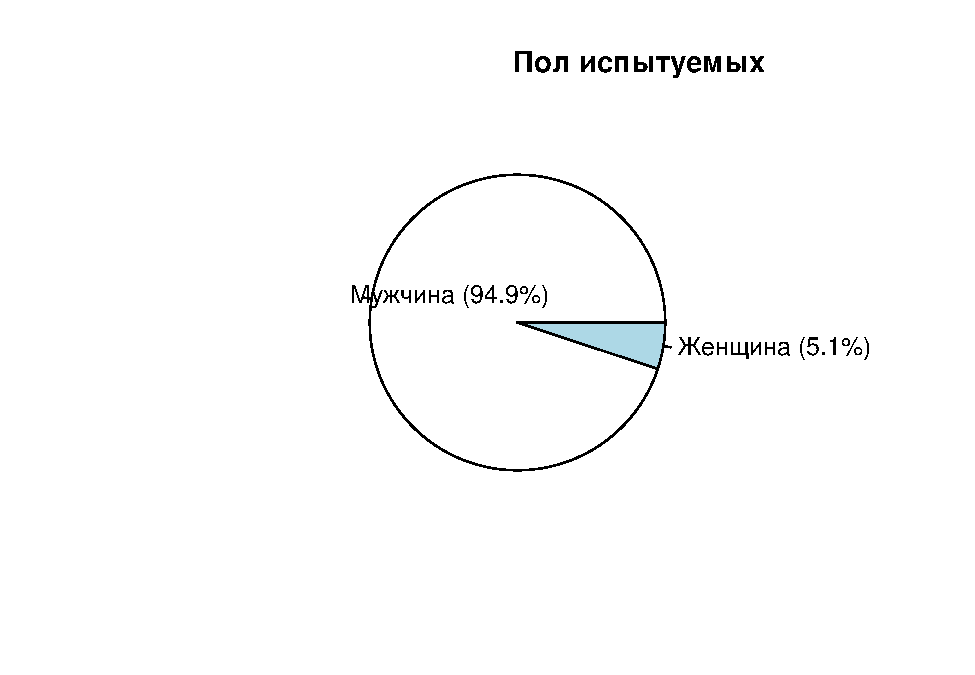
\includegraphics{Regression-model-for-estimating-RM_files/figure-latex/unnamed-chunk-4-1} \end{center}

Среди испытуемый почти половину составляли эндоморфы:

\begin{center}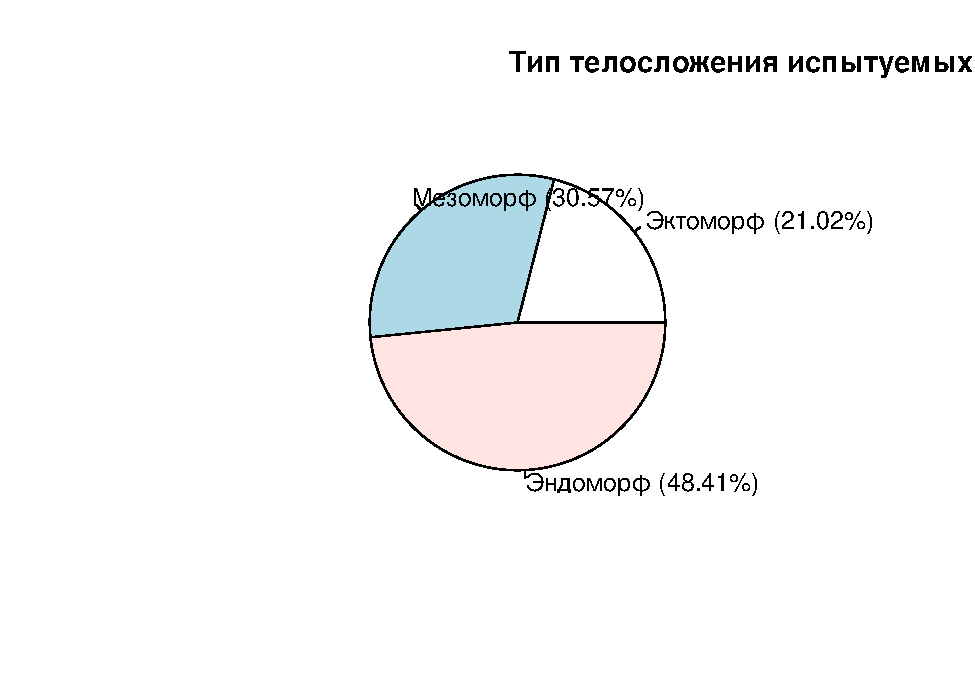
\includegraphics{Regression-model-for-estimating-RM_files/figure-latex/unnamed-chunk-5-1} \end{center}

и тест хи-квадрат говорит, что это отличие статистически значимо, то
есть \textbf{среди пауэрлифтеров эндоморфы встречаются чаще эктоморфов
или мезоморфов}:

\begin{longtable}[]{@{}ccc@{}}
\caption{Chi-squared test for given probabilities:
\texttt{data.unique\ \%\textgreater{}\%\ filter(Sex\ ==\ "Мужчина")\ \%\textgreater{}\%\ select(BodyType)\ \%\textgreater{}\%\ \ \ \ \ table()}}\tabularnewline
\toprule
\begin{minipage}[b]{0.22\columnwidth}\centering
Test statistic\strut
\end{minipage} & \begin{minipage}[b]{0.06\columnwidth}\centering
df\strut
\end{minipage} & \begin{minipage}[b]{0.23\columnwidth}\centering
P value\strut
\end{minipage}\tabularnewline
\midrule
\endfirsthead
\toprule
\begin{minipage}[b]{0.22\columnwidth}\centering
Test statistic\strut
\end{minipage} & \begin{minipage}[b]{0.06\columnwidth}\centering
df\strut
\end{minipage} & \begin{minipage}[b]{0.23\columnwidth}\centering
P value\strut
\end{minipage}\tabularnewline
\midrule
\endhead
\begin{minipage}[t]{0.22\columnwidth}\centering
16.28\strut
\end{minipage} & \begin{minipage}[t]{0.06\columnwidth}\centering
2\strut
\end{minipage} & \begin{minipage}[t]{0.23\columnwidth}\centering
0.0002914 * * *\strut
\end{minipage}\tabularnewline
\bottomrule
\end{longtable}

Больше половины наблюдений относятся к жиму лёжа. Я думаю, это связано с
тем, что большинство спортсменов просто предпочитают это упражнение двум
другим, вдобавок на жиме лёжа относительно проще замерять МПМ и, скорее
всего, многие из ответивших специализировались именно на жиме лёжа
(жимовики).

\begin{center}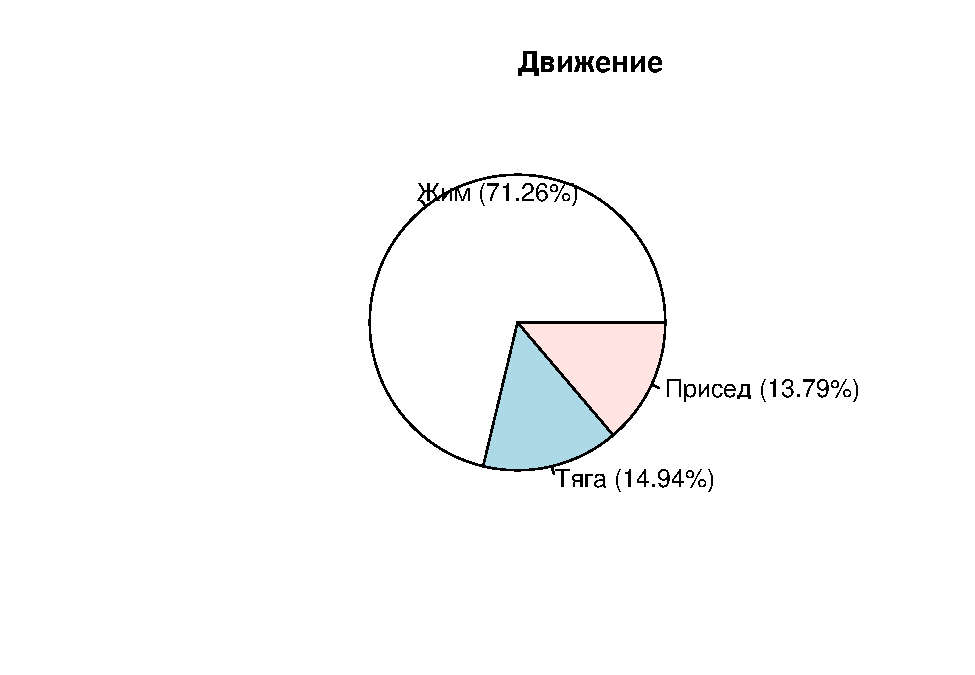
\includegraphics{Regression-model-for-estimating-RM_files/figure-latex/unnamed-chunk-7-1} \end{center}

\textbf{Распределение по другим факторам}:

\begin{center}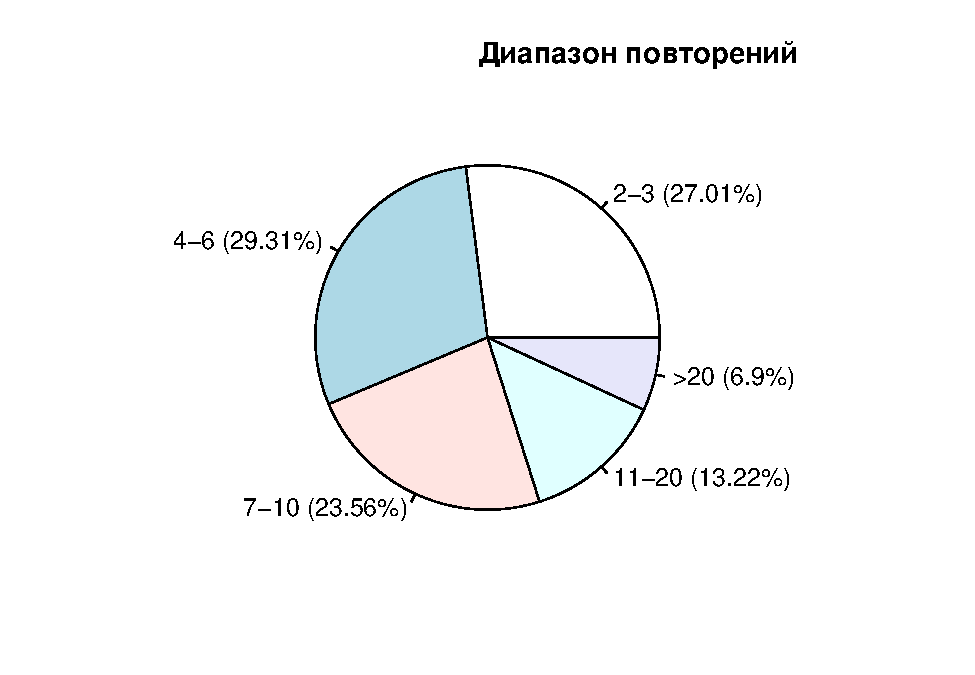
\includegraphics[width=0.85\linewidth]{Regression-model-for-estimating-RM_files/figure-latex/unnamed-chunk-8-1} \end{center}

\begin{center}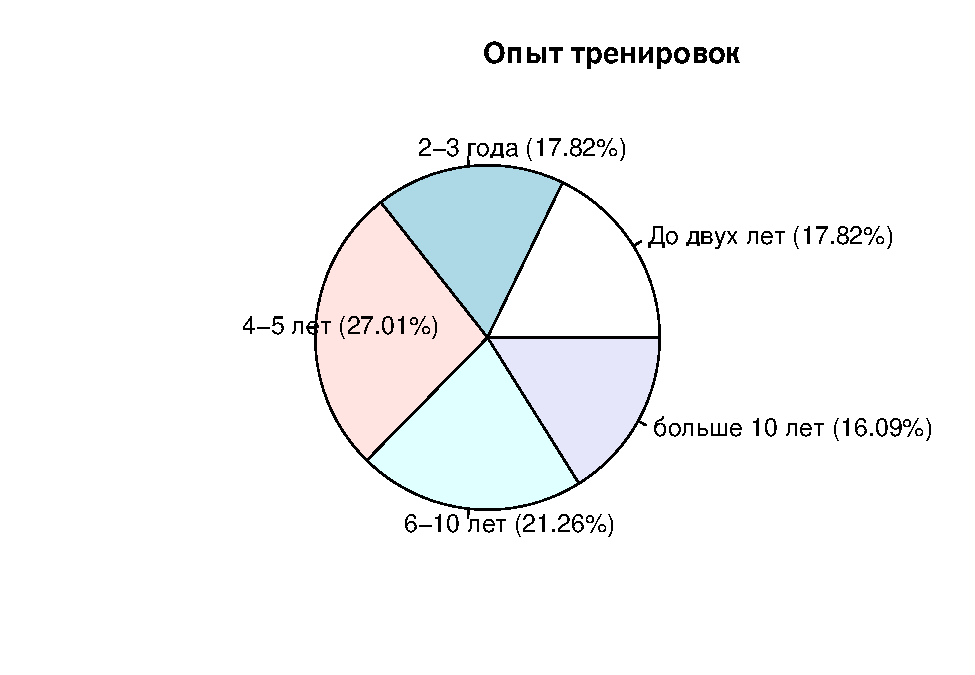
\includegraphics[width=0.85\linewidth]{Regression-model-for-estimating-RM_files/figure-latex/unnamed-chunk-8-2} \end{center}

\begin{center}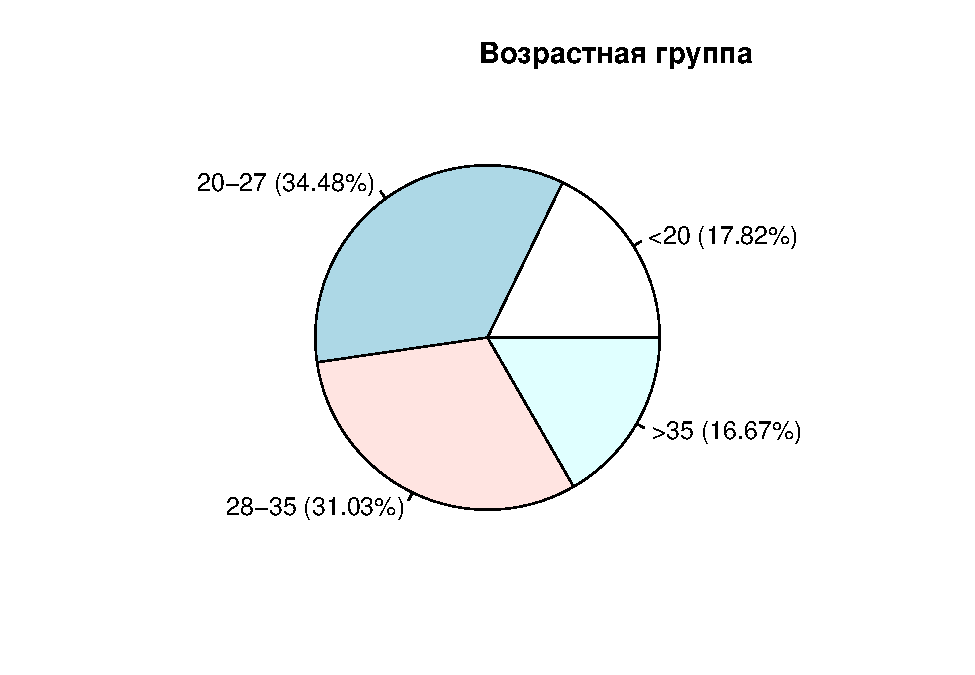
\includegraphics[width=0.85\linewidth]{Regression-model-for-estimating-RM_files/figure-latex/unnamed-chunk-8-3} \end{center}

\begin{center}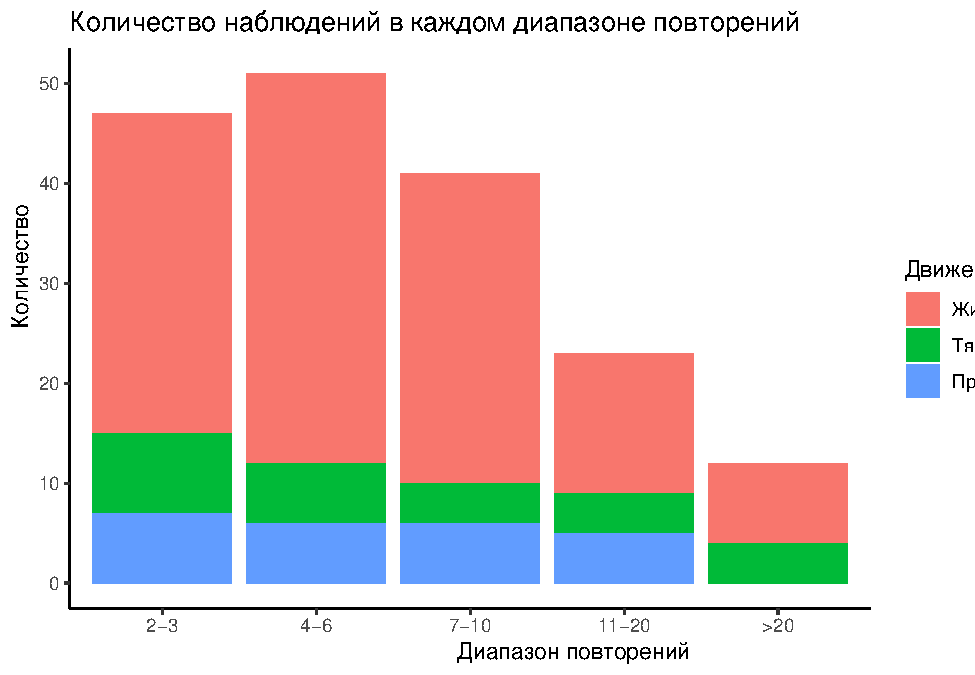
\includegraphics[width=0.85\linewidth]{Regression-model-for-estimating-RM_files/figure-latex/unnamed-chunk-8-4} \end{center}

\begin{center}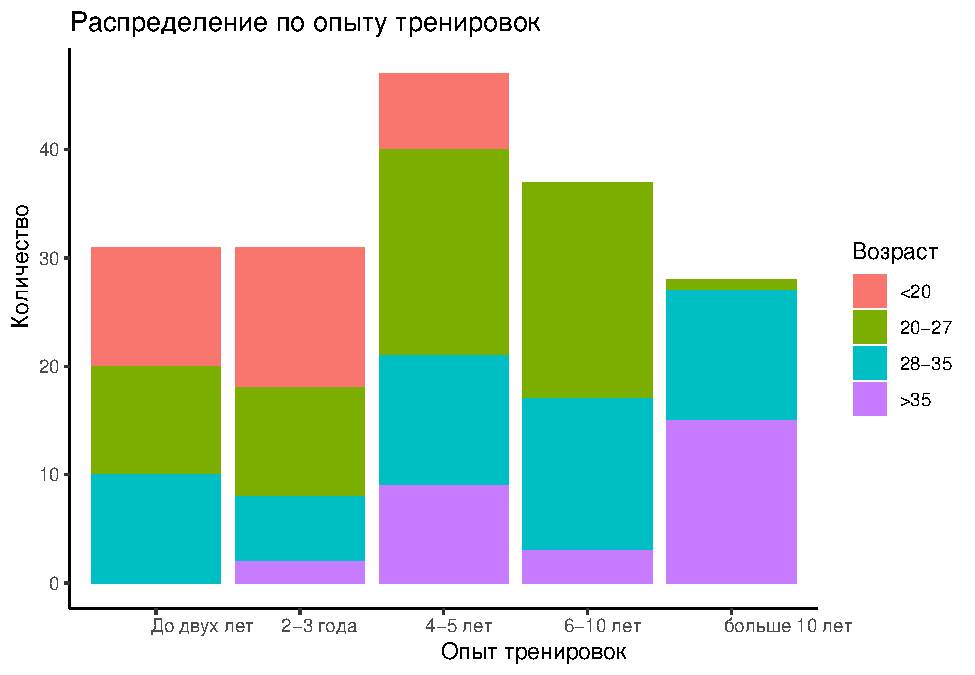
\includegraphics[width=0.85\linewidth]{Regression-model-for-estimating-RM_files/figure-latex/unnamed-chunk-8-5} \end{center}

\begin{center}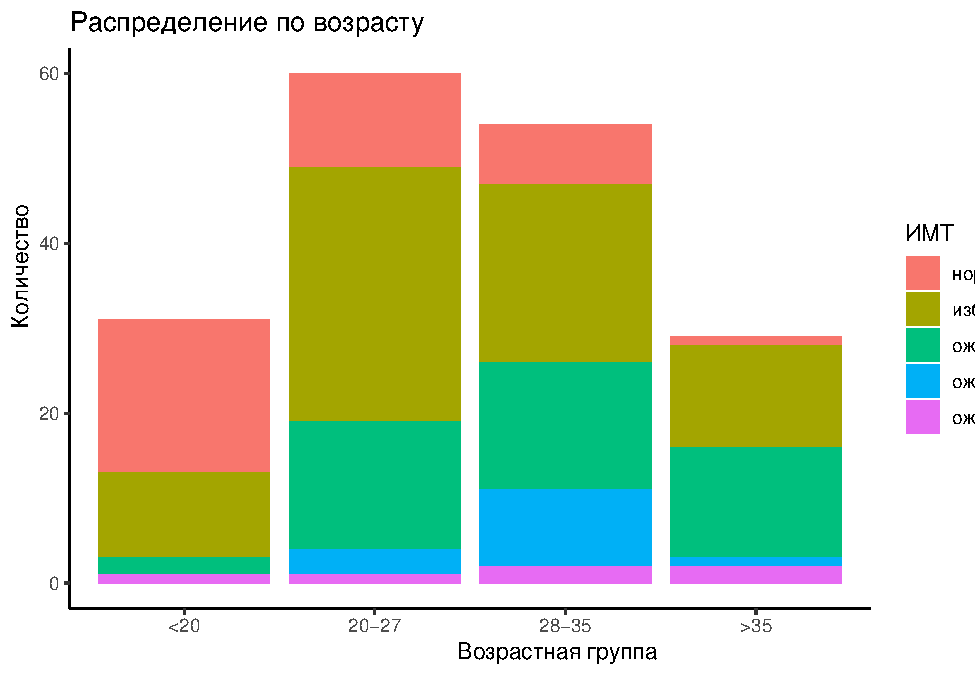
\includegraphics[width=0.85\linewidth]{Regression-model-for-estimating-RM_files/figure-latex/unnamed-chunk-8-6} \end{center}

\textbf{Распределение по индексу массы тела}:

\begin{longtable}[]{@{}lrrrrrrr@{}}
\toprule
& выраженный дефицит & дефицит & норма & избыток & ожирение1 & ожирение2
& ожирение3\tabularnewline
\midrule
\endhead
Эктоморф & 0 & 0 & 12 & 18 & 3 & 0 & 0\tabularnewline
Мезоморф & 0 & 0 & 19 & 23 & 5 & 1 & 0\tabularnewline
Эндоморф & 0 & 0 & 3 & 26 & 33 & 8 & 6\tabularnewline
\bottomrule
\end{longtable}

\begin{center}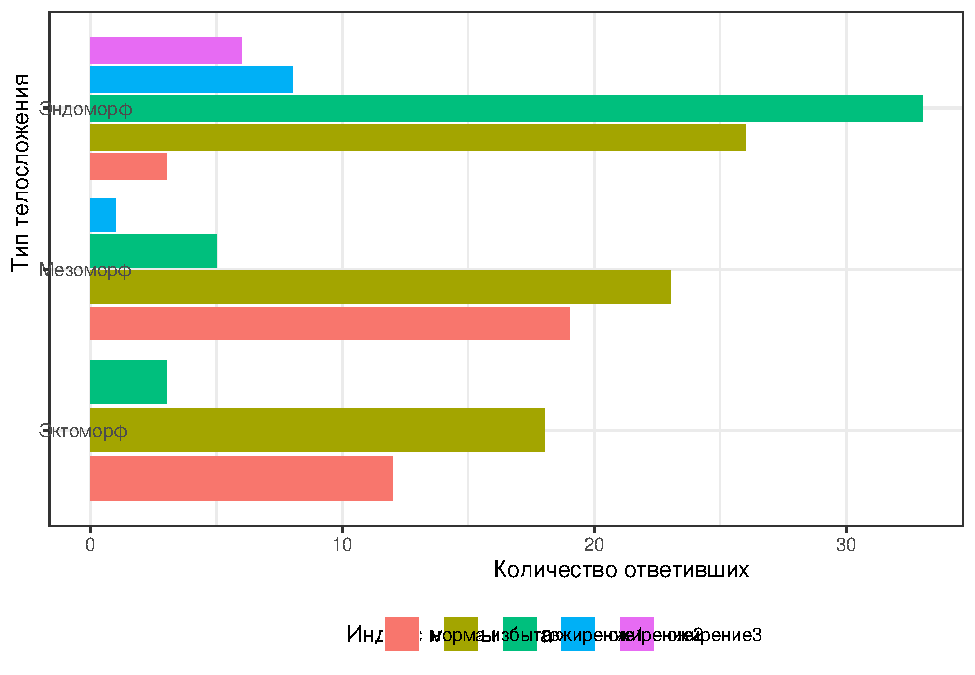
\includegraphics[width=0.9\linewidth]{Regression-model-for-estimating-RM_files/figure-latex/unnamed-chunk-9-1} \end{center}

Видно, что среди ответивших нет людей с дефицитом веса и немалая часть
имеет нормальный вес, немалая -- ``избыток'' (предположительно за счёт
мышечной массы), но так называемое \textbf{``ожирение1'' (с большой
вероятностью связанное с жировыми отложениями) у эндоморфов встречается
чаще, чем в других телосложениях}. Это подтверждает тест пропорций:

\begin{Shaded}
\begin{Highlighting}[]
\NormalTok{tb =}\StringTok{ }\NormalTok{data.unique }\OperatorTok\StringTok{ }\KeywordTok{mutate}\NormalTok{(}\DataTypeTok{Obees =} \KeywordTok{ifelse}\NormalTok{(IndexGroup }\OperatorTok{==}\StringTok{ "ожирение1"}\NormalTok{, }\StringTok{"да"}\NormalTok{, }\StringTok{"нет"}\NormalTok{)) }\OperatorTok\StringTok{ }
\StringTok{    }\KeywordTok{select}\NormalTok{(Obees, BodyType) }\OperatorTok\StringTok{ }\KeywordTok{table}\NormalTok{()}

\NormalTok{tb }\OperatorTok\StringTok{ }\KeywordTok{t}\NormalTok{() }\OperatorTok\StringTok{ }\KeywordTok{prop.test}\NormalTok{() }\OperatorTok\StringTok{ }\KeywordTok{pander}\NormalTok{()  }\CommentTok{#для всех}
\end{Highlighting}
\end{Shaded}

\begin{longtable}[]{@{}ccccc@{}}
\caption{3-sample test for equality of proportions without continuity
correction: \texttt{.} (continued below)}\tabularnewline
\toprule
\begin{minipage}[b]{0.19\columnwidth}\centering
Test statistic\strut
\end{minipage} & \begin{minipage}[b]{0.06\columnwidth}\centering
df\strut
\end{minipage} & \begin{minipage}[b]{0.21\columnwidth}\centering
P value\strut
\end{minipage} & \begin{minipage}[b]{0.29\columnwidth}\centering
Alternative hypothesis\strut
\end{minipage} & \begin{minipage}[b]{0.11\columnwidth}\centering
prop 1\strut
\end{minipage}\tabularnewline
\midrule
\endfirsthead
\toprule
\begin{minipage}[b]{0.19\columnwidth}\centering
Test statistic\strut
\end{minipage} & \begin{minipage}[b]{0.06\columnwidth}\centering
df\strut
\end{minipage} & \begin{minipage}[b]{0.21\columnwidth}\centering
P value\strut
\end{minipage} & \begin{minipage}[b]{0.29\columnwidth}\centering
Alternative hypothesis\strut
\end{minipage} & \begin{minipage}[b]{0.11\columnwidth}\centering
prop 1\strut
\end{minipage}\tabularnewline
\midrule
\endhead
\begin{minipage}[t]{0.19\columnwidth}\centering
22.88\strut
\end{minipage} & \begin{minipage}[t]{0.06\columnwidth}\centering
2\strut
\end{minipage} & \begin{minipage}[t]{0.21\columnwidth}\centering
1.073e-05 * * *\strut
\end{minipage} & \begin{minipage}[t]{0.29\columnwidth}\centering
two.sided\strut
\end{minipage} & \begin{minipage}[t]{0.11\columnwidth}\centering
0.09091\strut
\end{minipage}\tabularnewline
\bottomrule
\end{longtable}

\begin{longtable}[]{@{}cc@{}}
\toprule
\begin{minipage}[b]{0.12\columnwidth}\centering
prop 2\strut
\end{minipage} & \begin{minipage}[b]{0.12\columnwidth}\centering
prop 3\strut
\end{minipage}\tabularnewline
\midrule
\endhead
\begin{minipage}[t]{0.12\columnwidth}\centering
0.1042\strut
\end{minipage} & \begin{minipage}[t]{0.12\columnwidth}\centering
0.4342\strut
\end{minipage}\tabularnewline
\bottomrule
\end{longtable}

\begin{Shaded}
\begin{Highlighting}[]
\NormalTok{data.unique }\OperatorTok\StringTok{ }\KeywordTok{mutate}\NormalTok{(}\DataTypeTok{Obees =} \KeywordTok{ifelse}\NormalTok{(IndexGroup }\OperatorTok{==}\StringTok{ "ожирение1"}\NormalTok{, }\StringTok{"да"}\NormalTok{, }\StringTok{"нет"}\NormalTok{), }\DataTypeTok{Bd =} \KeywordTok{ifelse}\NormalTok{(BodyType }\OperatorTok{==}\StringTok{ }
\StringTok{    "Эндоморф"}\NormalTok{, }\DecValTok{1}\NormalTok{, }\DecValTok{0}\NormalTok{)) }\OperatorTok\StringTok{ }\KeywordTok{select}\NormalTok{(Obees, Bd) }\OperatorTok\StringTok{ }\KeywordTok{table}\NormalTok{() }\OperatorTok\StringTok{ }\KeywordTok{t}\NormalTok{() }\OperatorTok\StringTok{ }\KeywordTok{prop.test}\NormalTok{() }\OperatorTok\StringTok{ }
\StringTok{    }\KeywordTok{pander}\NormalTok{()  }\CommentTok{# eсли разделить на эндоморфов и всех остальных}
\end{Highlighting}
\end{Shaded}

\begin{longtable}[]{@{}cccccc@{}}
\caption{2-sample test for equality of proportions with continuity
correction: \texttt{.}}\tabularnewline
\toprule
\begin{minipage}[b]{0.17\columnwidth}\centering
Test statistic\strut
\end{minipage} & \begin{minipage}[b]{0.05\columnwidth}\centering
df\strut
\end{minipage} & \begin{minipage}[b]{0.18\columnwidth}\centering
P value\strut
\end{minipage} & \begin{minipage}[b]{0.24\columnwidth}\centering
Alternative hypothesis\strut
\end{minipage} & \begin{minipage}[b]{0.10\columnwidth}\centering
prop 1\strut
\end{minipage} & \begin{minipage}[b]{0.10\columnwidth}\centering
prop 2\strut
\end{minipage}\tabularnewline
\midrule
\endfirsthead
\toprule
\begin{minipage}[b]{0.17\columnwidth}\centering
Test statistic\strut
\end{minipage} & \begin{minipage}[b]{0.05\columnwidth}\centering
df\strut
\end{minipage} & \begin{minipage}[b]{0.18\columnwidth}\centering
P value\strut
\end{minipage} & \begin{minipage}[b]{0.24\columnwidth}\centering
Alternative hypothesis\strut
\end{minipage} & \begin{minipage}[b]{0.10\columnwidth}\centering
prop 1\strut
\end{minipage} & \begin{minipage}[b]{0.10\columnwidth}\centering
prop 2\strut
\end{minipage}\tabularnewline
\midrule
\endhead
\begin{minipage}[t]{0.17\columnwidth}\centering
21.16\strut
\end{minipage} & \begin{minipage}[t]{0.05\columnwidth}\centering
1\strut
\end{minipage} & \begin{minipage}[t]{0.18\columnwidth}\centering
4.223e-06 * * *\strut
\end{minipage} & \begin{minipage}[t]{0.24\columnwidth}\centering
two.sided\strut
\end{minipage} & \begin{minipage}[t]{0.10\columnwidth}\centering
0.09877\strut
\end{minipage} & \begin{minipage}[t]{0.10\columnwidth}\centering
0.4342\strut
\end{minipage}\tabularnewline
\bottomrule
\end{longtable}

Аналогично дисперсионный анализ показывает, что \textbf{эндоморфы имеют
больший ИМТ}:

\begin{Shaded}
\begin{Highlighting}[]
\KeywordTok{aov}\NormalTok{(Index }\OperatorTok{~}\StringTok{ }\NormalTok{BodyType, data) }\OperatorTok\StringTok{ }\KeywordTok{summary}\NormalTok{() }\OperatorTok\StringTok{ }\KeywordTok{pander}\NormalTok{()}
\end{Highlighting}
\end{Shaded}

\begin{longtable}[]{@{}cccccc@{}}
\caption{Analysis of Variance Model}\tabularnewline
\toprule
\begin{minipage}[b]{0.19\columnwidth}\centering
~\strut
\end{minipage} & \begin{minipage}[b]{0.07\columnwidth}\centering
Df\strut
\end{minipage} & \begin{minipage}[b]{0.10\columnwidth}\centering
Sum Sq\strut
\end{minipage} & \begin{minipage}[b]{0.12\columnwidth}\centering
Mean Sq\strut
\end{minipage} & \begin{minipage}[b]{0.12\columnwidth}\centering
F value\strut
\end{minipage} & \begin{minipage}[b]{0.14\columnwidth}\centering
Pr(\textgreater F)\strut
\end{minipage}\tabularnewline
\midrule
\endfirsthead
\toprule
\begin{minipage}[b]{0.19\columnwidth}\centering
~\strut
\end{minipage} & \begin{minipage}[b]{0.07\columnwidth}\centering
Df\strut
\end{minipage} & \begin{minipage}[b]{0.10\columnwidth}\centering
Sum Sq\strut
\end{minipage} & \begin{minipage}[b]{0.12\columnwidth}\centering
Mean Sq\strut
\end{minipage} & \begin{minipage}[b]{0.12\columnwidth}\centering
F value\strut
\end{minipage} & \begin{minipage}[b]{0.14\columnwidth}\centering
Pr(\textgreater F)\strut
\end{minipage}\tabularnewline
\midrule
\endhead
\begin{minipage}[t]{0.19\columnwidth}\centering
\textbf{BodyType}\strut
\end{minipage} & \begin{minipage}[t]{0.07\columnwidth}\centering
2\strut
\end{minipage} & \begin{minipage}[t]{0.10\columnwidth}\centering
1231\strut
\end{minipage} & \begin{minipage}[t]{0.12\columnwidth}\centering
615.6\strut
\end{minipage} & \begin{minipage}[t]{0.12\columnwidth}\centering
33.82\strut
\end{minipage} & \begin{minipage}[t]{0.14\columnwidth}\centering
4.201e-13\strut
\end{minipage}\tabularnewline
\begin{minipage}[t]{0.19\columnwidth}\centering
\textbf{Residuals}\strut
\end{minipage} & \begin{minipage}[t]{0.07\columnwidth}\centering
171\strut
\end{minipage} & \begin{minipage}[t]{0.10\columnwidth}\centering
3112\strut
\end{minipage} & \begin{minipage}[t]{0.12\columnwidth}\centering
18.2\strut
\end{minipage} & \begin{minipage}[t]{0.12\columnwidth}\centering
NA\strut
\end{minipage} & \begin{minipage}[t]{0.14\columnwidth}\centering
NA\strut
\end{minipage}\tabularnewline
\bottomrule
\end{longtable}

\begin{Shaded}
\begin{Highlighting}[]
\KeywordTok{t.test}\NormalTok{(data }\OperatorTok\StringTok{ }\KeywordTok{filter}\NormalTok{(BodyType }\OperatorTok{!=}\StringTok{ "Эндоморф"}\NormalTok{) }\OperatorTok\StringTok{ }\KeywordTok{select}\NormalTok{(Index) }\OperatorTok\StringTok{ }\KeywordTok{t}\NormalTok{() }\OperatorTok\StringTok{ }\KeywordTok{as.numeric}\NormalTok{(), }
\NormalTok{    data }\OperatorTok\StringTok{ }\KeywordTok{filter}\NormalTok{(BodyType }\OperatorTok{==}\StringTok{ "Эндоморф"}\NormalTok{) }\OperatorTok\StringTok{ }\KeywordTok{select}\NormalTok{(Index) }\OperatorTok\StringTok{ }\KeywordTok{t}\NormalTok{() }\OperatorTok\StringTok{ }\KeywordTok{as.numeric}\NormalTok{()) }\OperatorTok\StringTok{ }
\StringTok{    }\KeywordTok{pander}\NormalTok{()}
\end{Highlighting}
\end{Shaded}

\begin{longtable}[]{@{}ccccc@{}}
\caption{Welch Two Sample t-test:
\texttt{data\ \%\textgreater{}\%\ filter(BodyType\ !=\ "Эндоморф")\ \%\textgreater{}\%\ select(Index)\ \%\textgreater{}\%}
and
\texttt{data\ \%\textgreater{}\%\ filter(BodyType\ ==\ "Эндоморф")\ \%\textgreater{}\%\ select(Index)\ \%\textgreater{}\%\ \ \ \ \ t()\ \%\textgreater{}\%\ as.numeric()}
and \texttt{t()\ \%\textgreater{}\%\ as.numeric()} (continued
below)}\tabularnewline
\toprule
\begin{minipage}[b]{0.18\columnwidth}\centering
Test statistic\strut
\end{minipage} & \begin{minipage}[b]{0.09\columnwidth}\centering
df\strut
\end{minipage} & \begin{minipage}[b]{0.19\columnwidth}\centering
P value\strut
\end{minipage} & \begin{minipage}[b]{0.27\columnwidth}\centering
Alternative hypothesis\strut
\end{minipage} & \begin{minipage}[b]{0.13\columnwidth}\centering
mean of x\strut
\end{minipage}\tabularnewline
\midrule
\endfirsthead
\toprule
\begin{minipage}[b]{0.18\columnwidth}\centering
Test statistic\strut
\end{minipage} & \begin{minipage}[b]{0.09\columnwidth}\centering
df\strut
\end{minipage} & \begin{minipage}[b]{0.19\columnwidth}\centering
P value\strut
\end{minipage} & \begin{minipage}[b]{0.27\columnwidth}\centering
Alternative hypothesis\strut
\end{minipage} & \begin{minipage}[b]{0.13\columnwidth}\centering
mean of x\strut
\end{minipage}\tabularnewline
\midrule
\endhead
\begin{minipage}[t]{0.18\columnwidth}\centering
-8.105\strut
\end{minipage} & \begin{minipage}[t]{0.09\columnwidth}\centering
152.2\strut
\end{minipage} & \begin{minipage}[t]{0.19\columnwidth}\centering
1.608e-13 * * *\strut
\end{minipage} & \begin{minipage}[t]{0.27\columnwidth}\centering
two.sided\strut
\end{minipage} & \begin{minipage}[t]{0.13\columnwidth}\centering
25.87\strut
\end{minipage}\tabularnewline
\bottomrule
\end{longtable}

\begin{longtable}[]{@{}c@{}}
\toprule
\begin{minipage}[b]{0.16\columnwidth}\centering
mean of y\strut
\end{minipage}\tabularnewline
\midrule
\endhead
\begin{minipage}[t]{0.16\columnwidth}\centering
31.14\strut
\end{minipage}\tabularnewline
\bottomrule
\end{longtable}

\hypertarget{ux432ux437ux430ux438ux43cux43eux434ux435ux441ux442ux432ux438ux44f-ux43fux435ux440ux435ux43cux435ux43dux43dux44bux445}{%
\subsection{Взаимодествия
переменных}\label{ux432ux437ux430ux438ux43cux43eux434ux435ux441ux442ux432ux438ux44f-ux43fux435ux440ux435ux43cux435ux43dux43dux44bux445}}

Иллюстрация некоторых парных взаимодействий:

\begin{center}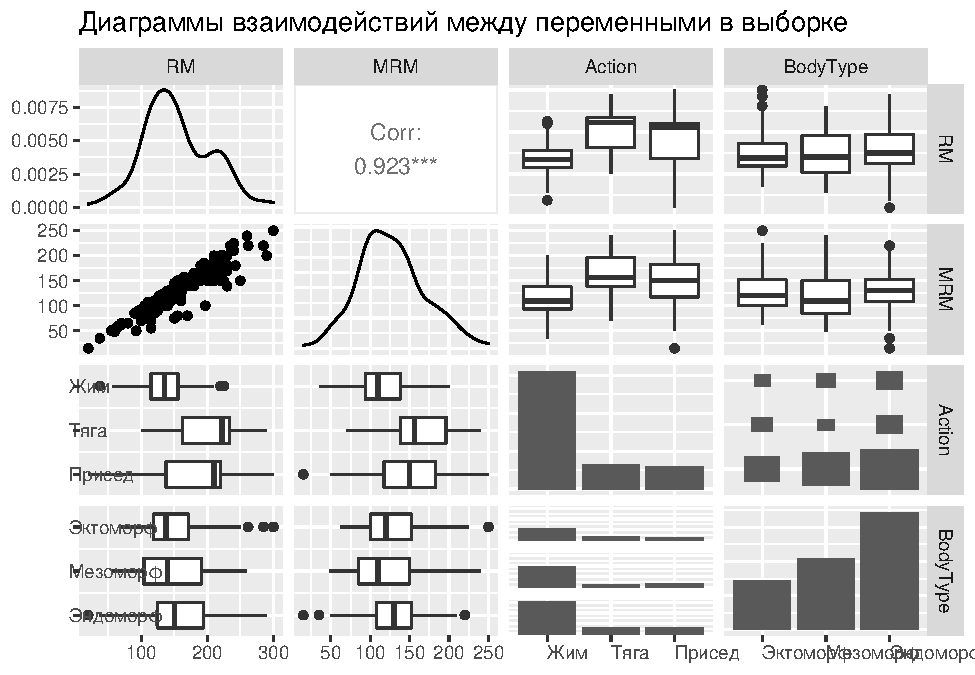
\includegraphics[width=0.95\linewidth]{Regression-model-for-estimating-RM_files/figure-latex/unnamed-chunk-12-1} \end{center}

\textbf{Корреляции количественных переменных}:

\begin{center}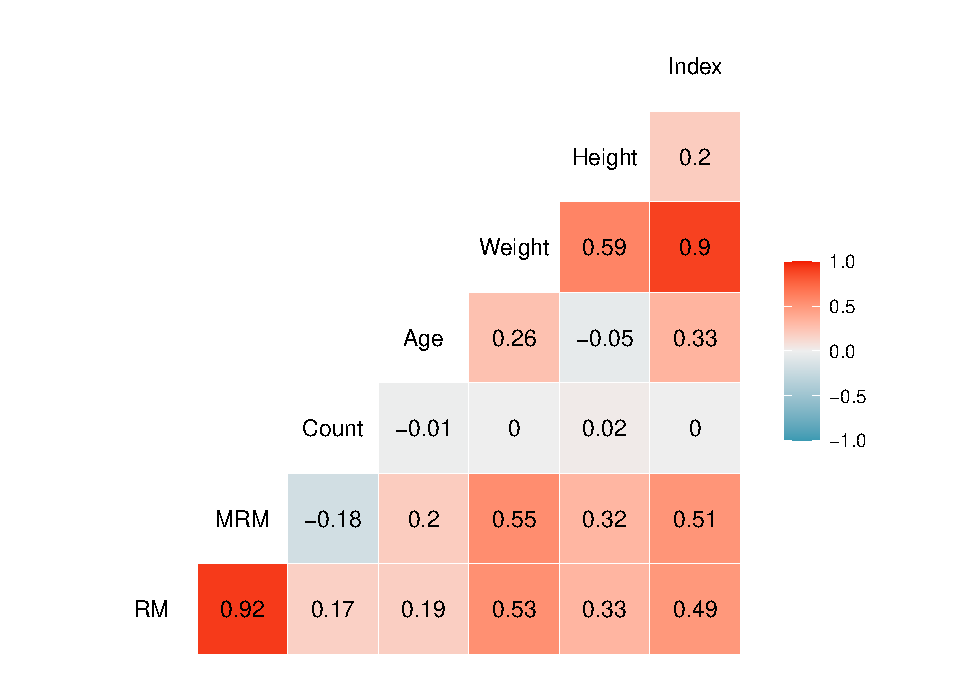
\includegraphics{Regression-model-for-estimating-RM_files/figure-latex/unnamed-chunk-13-1} \end{center}

Зависимость повторного максимума от индекса массы тела:

\begin{center}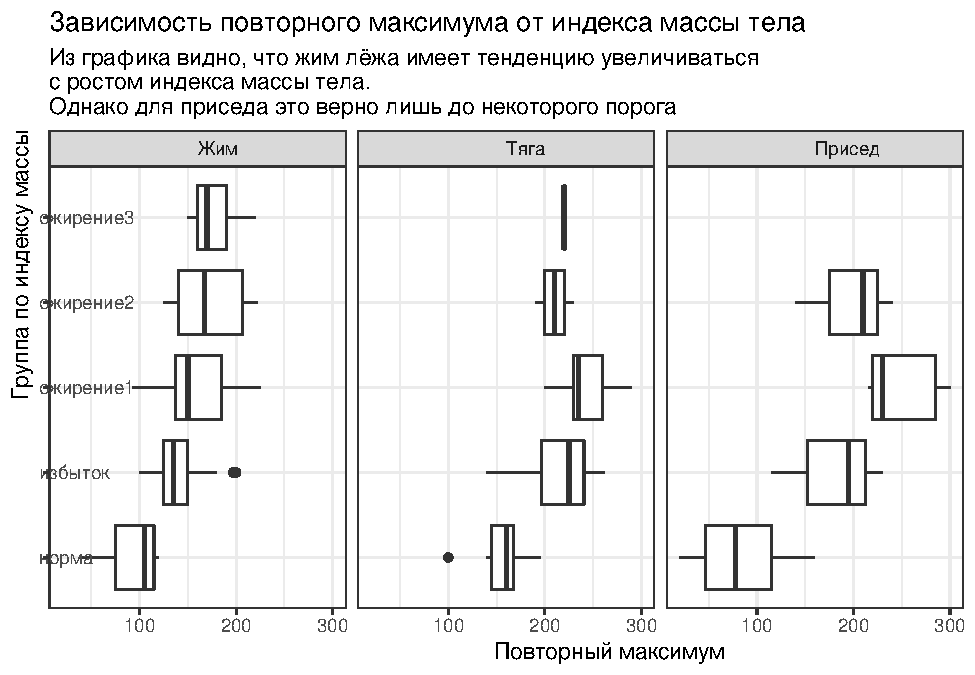
\includegraphics[width=0.9\linewidth]{Regression-model-for-estimating-RM_files/figure-latex/unnamed-chunk-14-1} \end{center}

\begin{center}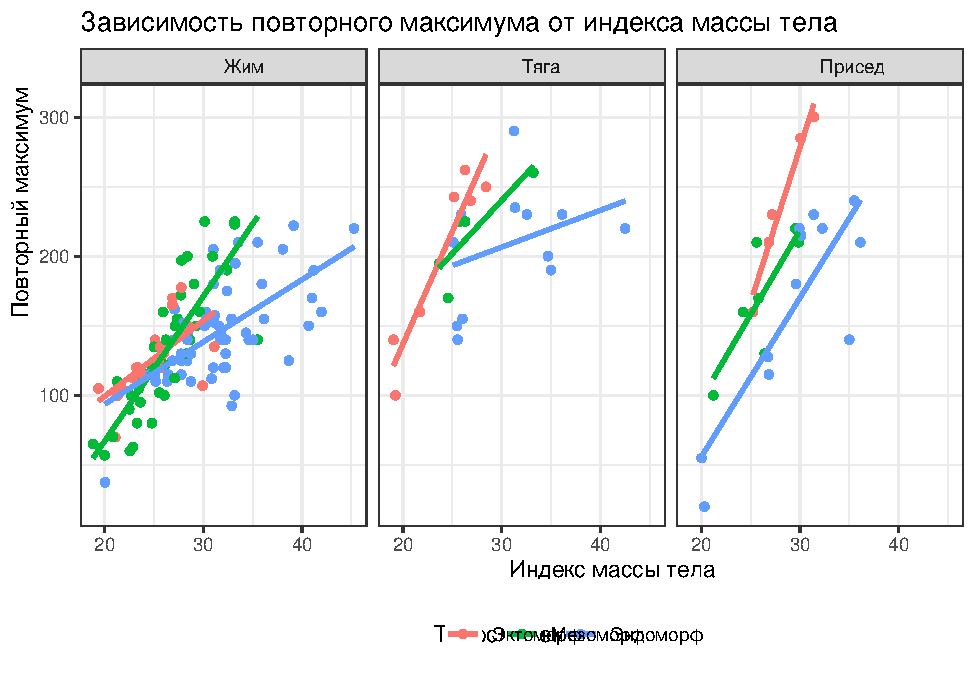
\includegraphics[width=0.9\linewidth]{Regression-model-for-estimating-RM_files/figure-latex/unnamed-chunk-14-2} \end{center}

Оценка коэффициента простой регрессионной модели в зависимости от числа
повторений:

\begin{center}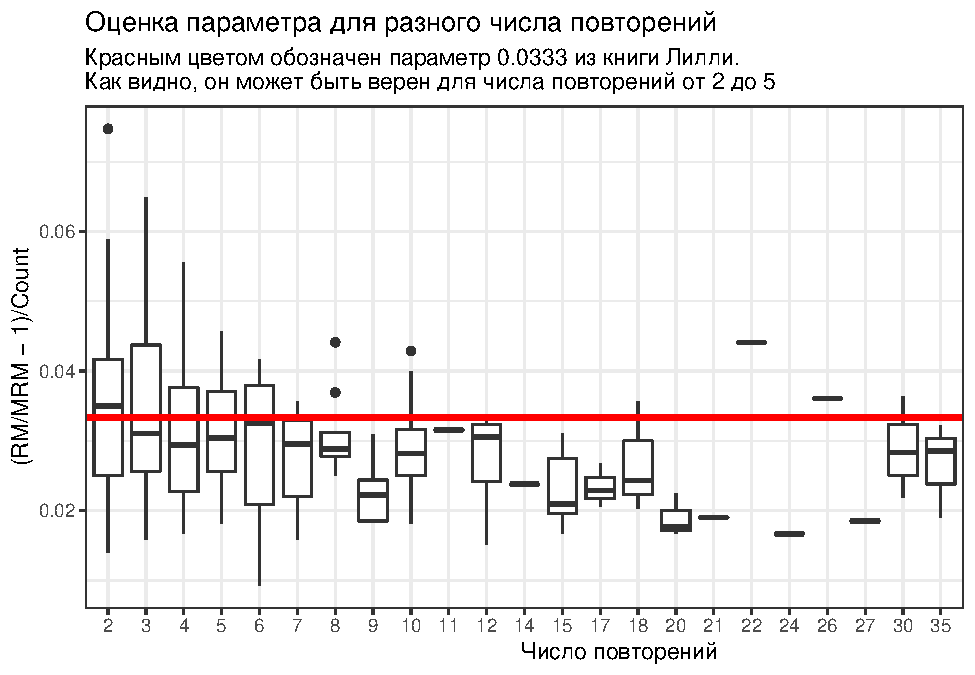
\includegraphics[width=0.9\linewidth]{Regression-model-for-estimating-RM_files/figure-latex/unnamed-chunk-15-1} \end{center}

Из следующего графика может следовать, что начиная с 8-9 повторений
зависимость между МПМ и ПМ ослабевает:

\begin{center}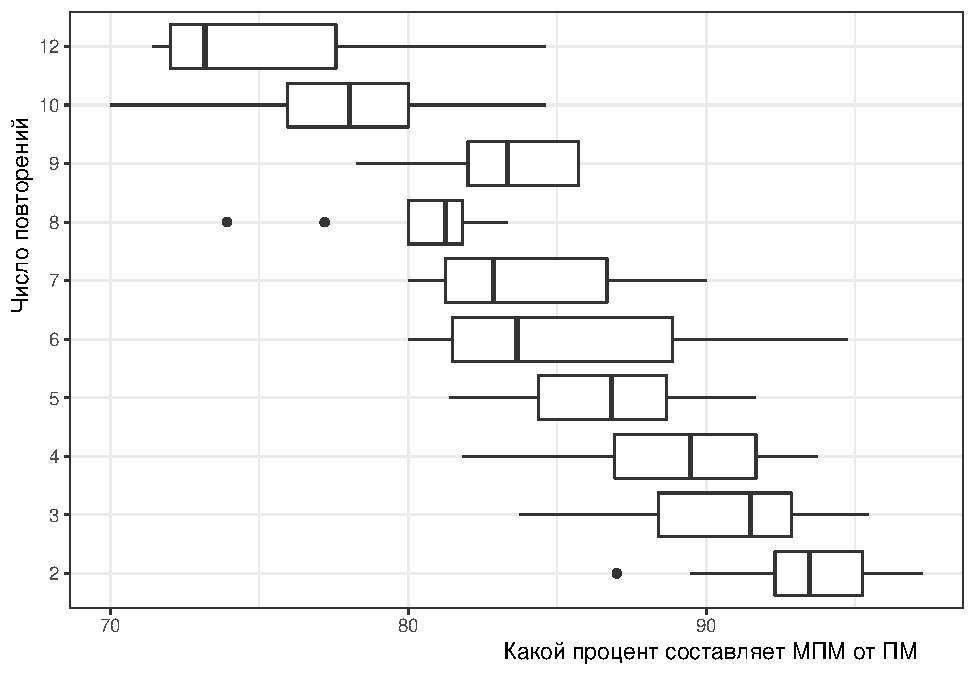
\includegraphics{Regression-model-for-estimating-RM_files/figure-latex/unnamed-chunk-16-1} \end{center}

Либо здесь имеется проблема с данными, так как на 9-м повторении
корреляция резко уменьшается (мало наблюдений):

\begin{Shaded}
\begin{Highlighting}[]
\KeywordTok{tibble}\NormalTok{(}\StringTok{`}\DataTypeTok{Число повторений}\StringTok{`}\NormalTok{ =}\StringTok{ }\DecValTok{2}\OperatorTok{:}\DecValTok{10}\NormalTok{, }\StringTok{`}\DataTypeTok{Корреляция MRM & RM}\StringTok{`}\NormalTok{ =}\StringTok{ }\KeywordTok{sapply}\NormalTok{(}\DecValTok{2}\OperatorTok{:}\DecValTok{10}\NormalTok{, }\ControlFlowTok{function}\NormalTok{(x) data }\OperatorTok\StringTok{ }
\StringTok{    }\KeywordTok{filter}\NormalTok{(Count }\OperatorTok{==}\StringTok{ }\NormalTok{x) }\OperatorTok\StringTok{ }\KeywordTok{cor}\NormalTok{(RM, MRM)), }\StringTok{`}\DataTypeTok{Нижняя граница}\StringTok{`}\NormalTok{ =}\StringTok{ }\KeywordTok{sapply}\NormalTok{(}\DecValTok{2}\OperatorTok{:}\DecValTok{10}\NormalTok{, }\ControlFlowTok{function}\NormalTok{(x) data }\OperatorTok\StringTok{ }
\StringTok{    }\KeywordTok{filter}\NormalTok{(Count }\OperatorTok{==}\StringTok{ }\NormalTok{x) }\OperatorTok\StringTok{ }\KeywordTok{cor.test}\NormalTok{(RM, MRM)}\OperatorTok{$}\NormalTok{conf.int[}\DecValTok{1}\NormalTok{]), }\StringTok{`}\DataTypeTok{Верхняя граница}\StringTok{`}\NormalTok{ =}\StringTok{ }\KeywordTok{sapply}\NormalTok{(}\DecValTok{2}\OperatorTok{:}\DecValTok{10}\NormalTok{, }
    \ControlFlowTok{function}\NormalTok{(x) data }\OperatorTok\StringTok{ }\KeywordTok{filter}\NormalTok{(Count }\OperatorTok{==}\StringTok{ }\NormalTok{x) }\OperatorTok\StringTok{ }\KeywordTok{cor.test}\NormalTok{(RM, MRM)}\OperatorTok{$}\NormalTok{conf.int[}\DecValTok{2}\NormalTok{]), }\StringTok{`}\DataTypeTok{Всего наблюдений}\StringTok{`}\NormalTok{ =}\StringTok{ }\KeywordTok{sapply}\NormalTok{(}\DecValTok{2}\OperatorTok{:}\DecValTok{10}\NormalTok{, }
    \ControlFlowTok{function}\NormalTok{(x) data }\OperatorTok\StringTok{ }\KeywordTok{filter}\NormalTok{(Count }\OperatorTok{==}\StringTok{ }\NormalTok{x) }\OperatorTok\StringTok{ }\KeywordTok{nrow}\NormalTok{())) }\OperatorTok\StringTok{ }\KeywordTok{kable}\NormalTok{(}\DataTypeTok{caption =} \StringTok{"Корреляция между MRM & RM для каждого повторения"}\NormalTok{, }
    \DataTypeTok{align =} \StringTok{"ccccc"}\NormalTok{)}
\end{Highlighting}
\end{Shaded}

\begin{longtable}[]{@{}ccccc@{}}
\caption{Корреляция между MRM \& RM для каждого
повторения}\tabularnewline
\toprule
\begin{minipage}[b]{0.17\columnwidth}\centering
Число повторений\strut
\end{minipage} & \begin{minipage}[b]{0.20\columnwidth}\centering
Корреляция MRM \& RM\strut
\end{minipage} & \begin{minipage}[b]{0.15\columnwidth}\centering
Нижняя граница\strut
\end{minipage} & \begin{minipage}[b]{0.16\columnwidth}\centering
Верхняя граница\strut
\end{minipage} & \begin{minipage}[b]{0.17\columnwidth}\centering
Всего наблюдений\strut
\end{minipage}\tabularnewline
\midrule
\endfirsthead
\toprule
\begin{minipage}[b]{0.17\columnwidth}\centering
Число повторений\strut
\end{minipage} & \begin{minipage}[b]{0.20\columnwidth}\centering
Корреляция MRM \& RM\strut
\end{minipage} & \begin{minipage}[b]{0.15\columnwidth}\centering
Нижняя граница\strut
\end{minipage} & \begin{minipage}[b]{0.16\columnwidth}\centering
Верхняя граница\strut
\end{minipage} & \begin{minipage}[b]{0.17\columnwidth}\centering
Всего наблюдений\strut
\end{minipage}\tabularnewline
\midrule
\endhead
\begin{minipage}[t]{0.17\columnwidth}\centering
2\strut
\end{minipage} & \begin{minipage}[t]{0.20\columnwidth}\centering
0.9980117\strut
\end{minipage} & \begin{minipage}[t]{0.15\columnwidth}\centering
0.9949986\strut
\end{minipage} & \begin{minipage}[t]{0.16\columnwidth}\centering
0.9992103\strut
\end{minipage} & \begin{minipage}[t]{0.17\columnwidth}\centering
21\strut
\end{minipage}\tabularnewline
\begin{minipage}[t]{0.17\columnwidth}\centering
3\strut
\end{minipage} & \begin{minipage}[t]{0.20\columnwidth}\centering
0.9919420\strut
\end{minipage} & \begin{minipage}[t]{0.15\columnwidth}\centering
0.9818449\strut
\end{minipage} & \begin{minipage}[t]{0.16\columnwidth}\centering
0.9964336\strut
\end{minipage} & \begin{minipage}[t]{0.17\columnwidth}\centering
26\strut
\end{minipage}\tabularnewline
\begin{minipage}[t]{0.17\columnwidth}\centering
4\strut
\end{minipage} & \begin{minipage}[t]{0.20\columnwidth}\centering
0.9947569\strut
\end{minipage} & \begin{minipage}[t]{0.15\columnwidth}\centering
0.9838325\strut
\end{minipage} & \begin{minipage}[t]{0.16\columnwidth}\centering
0.9983060\strut
\end{minipage} & \begin{minipage}[t]{0.17\columnwidth}\centering
15\strut
\end{minipage}\tabularnewline
\begin{minipage}[t]{0.17\columnwidth}\centering
5\strut
\end{minipage} & \begin{minipage}[t]{0.20\columnwidth}\centering
0.9891096\strut
\end{minipage} & \begin{minipage}[t]{0.15\columnwidth}\centering
0.9734436\strut
\end{minipage} & \begin{minipage}[t]{0.16\columnwidth}\centering
0.9955548\strut
\end{minipage} & \begin{minipage}[t]{0.17\columnwidth}\centering
22\strut
\end{minipage}\tabularnewline
\begin{minipage}[t]{0.17\columnwidth}\centering
6\strut
\end{minipage} & \begin{minipage}[t]{0.20\columnwidth}\centering
0.9942644\strut
\end{minipage} & \begin{minipage}[t]{0.15\columnwidth}\centering
0.9814191\strut
\end{minipage} & \begin{minipage}[t]{0.16\columnwidth}\centering
0.9982374\strut
\end{minipage} & \begin{minipage}[t]{0.17\columnwidth}\centering
14\strut
\end{minipage}\tabularnewline
\begin{minipage}[t]{0.17\columnwidth}\centering
7\strut
\end{minipage} & \begin{minipage}[t]{0.20\columnwidth}\centering
0.9936119\strut
\end{minipage} & \begin{minipage}[t]{0.15\columnwidth}\centering
0.9687446\strut
\end{minipage} & \begin{minipage}[t]{0.16\columnwidth}\centering
0.9987074\strut
\end{minipage} & \begin{minipage}[t]{0.17\columnwidth}\centering
9\strut
\end{minipage}\tabularnewline
\begin{minipage}[t]{0.17\columnwidth}\centering
8\strut
\end{minipage} & \begin{minipage}[t]{0.20\columnwidth}\centering
0.9964144\strut
\end{minipage} & \begin{minipage}[t]{0.15\columnwidth}\centering
0.9876689\strut
\end{minipage} & \begin{minipage}[t]{0.16\columnwidth}\centering
0.9989606\strut
\end{minipage} & \begin{minipage}[t]{0.17\columnwidth}\centering
13\strut
\end{minipage}\tabularnewline
\begin{minipage}[t]{0.17\columnwidth}\centering
9\strut
\end{minipage} & \begin{minipage}[t]{0.20\columnwidth}\centering
0.9581086\strut
\end{minipage} & \begin{minipage}[t]{0.15\columnwidth}\centering
0.4902757\strut
\end{minipage} & \begin{minipage}[t]{0.16\columnwidth}\centering
0.9973273\strut
\end{minipage} & \begin{minipage}[t]{0.17\columnwidth}\centering
5\strut
\end{minipage}\tabularnewline
\begin{minipage}[t]{0.17\columnwidth}\centering
10\strut
\end{minipage} & \begin{minipage}[t]{0.20\columnwidth}\centering
0.9890079\strut
\end{minipage} & \begin{minipage}[t]{0.15\columnwidth}\centering
0.9645992\strut
\end{minipage} & \begin{minipage}[t]{0.16\columnwidth}\centering
0.9966159\strut
\end{minipage} & \begin{minipage}[t]{0.17\columnwidth}\centering
14\strut
\end{minipage}\tabularnewline
\bottomrule
\end{longtable}

\textbf{Есть ли разница в этих процентах для разных движений или
телосложений? Дисперсионный анализ показывает, что нет}, значимых
различий не обнаружено (все p-значения больше 0.05):

\begin{Shaded}
\begin{Highlighting}[]
\CommentTok{# есть ли разница в проценте в зависимости от чего-то}

\CommentTok{# cat('p-значения для телосложений:\textbackslash{}n')}
\NormalTok{pvalues1 =}\StringTok{ }\KeywordTok{sapply}\NormalTok{(}\DecValTok{2}\OperatorTok{:}\DecValTok{10}\NormalTok{, }\ControlFlowTok{function}\NormalTok{(x) data }\OperatorTok\StringTok{ }\KeywordTok{filter}\NormalTok{(Count }\OperatorTok{==}\StringTok{ }\NormalTok{x) }\OperatorTok\StringTok{ }\KeywordTok{aov}\NormalTok{(MRM}\OperatorTok{/}\NormalTok{RM }\OperatorTok{~}\StringTok{ }
\StringTok{    }\NormalTok{BodyType, .) }\OperatorTok\StringTok{ }\KeywordTok{summary}\NormalTok{() }\OperatorTok\StringTok{ }\NormalTok{.[[}\DecValTok{1}\NormalTok{]][[}\StringTok{"Pr(>F)"}\NormalTok{]][}\DecValTok{1}\NormalTok{])}
\KeywordTok{names}\NormalTok{(pvalues1) =}\StringTok{ }\KeywordTok{paste}\NormalTok{(}\DecValTok{2}\OperatorTok{:}\DecValTok{10}\NormalTok{, }\StringTok{"repeats"}\NormalTok{)}


\CommentTok{# cat('p-значения для типа движения:\textbackslash{}n')}
\NormalTok{pvalues2 =}\StringTok{ }\KeywordTok{sapply}\NormalTok{(}\DecValTok{2}\OperatorTok{:}\DecValTok{6}\NormalTok{, }\ControlFlowTok{function}\NormalTok{(x) data }\OperatorTok\StringTok{ }\KeywordTok{filter}\NormalTok{(Count }\OperatorTok{==}\StringTok{ }\NormalTok{x) }\OperatorTok\StringTok{ }\KeywordTok{aov}\NormalTok{(MRM}\OperatorTok{/}\NormalTok{RM }\OperatorTok{~}\StringTok{ }\NormalTok{Action, }
\NormalTok{    .) }\OperatorTok\StringTok{ }\KeywordTok{summary}\NormalTok{() }\OperatorTok\StringTok{ }\NormalTok{.[[}\DecValTok{1}\NormalTok{]][[}\StringTok{"Pr(>F)"}\NormalTok{]][}\DecValTok{1}\NormalTok{]) }\OperatorTok\StringTok{ }\KeywordTok{round}\NormalTok{(}\DecValTok{7}\NormalTok{)}
\KeywordTok{names}\NormalTok{(pvalues2) =}\StringTok{ }\KeywordTok{paste}\NormalTok{(}\DecValTok{2}\OperatorTok{:}\DecValTok{6}\NormalTok{, }\StringTok{"repeats"}\NormalTok{)}


\CommentTok{# cat('p-значения для групп по индексу массы:\textbackslash{}n')}
\NormalTok{pvalues3 =}\StringTok{ }\KeywordTok{sapply}\NormalTok{(}\DecValTok{2}\OperatorTok{:}\DecValTok{10}\NormalTok{, }\ControlFlowTok{function}\NormalTok{(x) data }\OperatorTok\StringTok{ }\KeywordTok{filter}\NormalTok{(Count }\OperatorTok{==}\StringTok{ }\NormalTok{x) }\OperatorTok\StringTok{ }\KeywordTok{aov}\NormalTok{(MRM}\OperatorTok{/}\NormalTok{RM }\OperatorTok{~}\StringTok{ }
\StringTok{    }\NormalTok{IndexGroup, .) }\OperatorTok\StringTok{ }\KeywordTok{summary}\NormalTok{() }\OperatorTok\StringTok{ }\NormalTok{.[[}\DecValTok{1}\NormalTok{]][[}\StringTok{"Pr(>F)"}\NormalTok{]][}\DecValTok{1}\NormalTok{])}
\KeywordTok{names}\NormalTok{(pvalues3) =}\StringTok{ }\KeywordTok{paste}\NormalTok{(}\DecValTok{2}\OperatorTok{:}\DecValTok{10}\NormalTok{, }\StringTok{"repeats"}\NormalTok{)}


\KeywordTok{tibble}\NormalTok{(}\StringTok{`}\DataTypeTok{Число повторений}\StringTok{`}\NormalTok{ =}\StringTok{ }\DecValTok{2}\OperatorTok{:}\DecValTok{10}\NormalTok{, }\StringTok{`}\DataTypeTok{p-значения для телосложений}\StringTok{`}\NormalTok{ =}\StringTok{ }\NormalTok{pvalues1, }\StringTok{`}\DataTypeTok{p-значения для типа движения}\StringTok{`}\NormalTok{ =}\StringTok{ }\KeywordTok{c}\NormalTok{(pvalues2, }
    \KeywordTok{rep}\NormalTok{(}\StringTok{"мало данных"}\NormalTok{, }\DecValTok{4}\NormalTok{)), }\StringTok{`}\DataTypeTok{p-значения для групп по индексу массы}\StringTok{`}\NormalTok{ =}\StringTok{ }\NormalTok{pvalues3) }\OperatorTok\StringTok{ }
\StringTok{    }\KeywordTok{kable}\NormalTok{(}\DataTypeTok{caption =} \StringTok{"p-значения для разных факторных переменных на каждом числе повторений"}\NormalTok{, }
        \DataTypeTok{align =} \StringTok{"cccc"}\NormalTok{)}
\end{Highlighting}
\end{Shaded}

\begin{longtable}[]{@{}cccc@{}}
\caption{p-значения для разных факторных переменных на каждом числе
повторений}\tabularnewline
\toprule
\begin{minipage}[b]{0.14\columnwidth}\centering
Число повторений\strut
\end{minipage} & \begin{minipage}[b]{0.22\columnwidth}\centering
p-значения для телосложений\strut
\end{minipage} & \begin{minipage}[b]{0.23\columnwidth}\centering
p-значения для типа движения\strut
\end{minipage} & \begin{minipage}[b]{0.30\columnwidth}\centering
p-значения для групп по индексу массы\strut
\end{minipage}\tabularnewline
\midrule
\endfirsthead
\toprule
\begin{minipage}[b]{0.14\columnwidth}\centering
Число повторений\strut
\end{minipage} & \begin{minipage}[b]{0.22\columnwidth}\centering
p-значения для телосложений\strut
\end{minipage} & \begin{minipage}[b]{0.23\columnwidth}\centering
p-значения для типа движения\strut
\end{minipage} & \begin{minipage}[b]{0.30\columnwidth}\centering
p-значения для групп по индексу массы\strut
\end{minipage}\tabularnewline
\midrule
\endhead
\begin{minipage}[t]{0.14\columnwidth}\centering
2\strut
\end{minipage} & \begin{minipage}[t]{0.22\columnwidth}\centering
0.9458770\strut
\end{minipage} & \begin{minipage}[t]{0.23\columnwidth}\centering
0.7730952\strut
\end{minipage} & \begin{minipage}[t]{0.30\columnwidth}\centering
0.8959581\strut
\end{minipage}\tabularnewline
\begin{minipage}[t]{0.14\columnwidth}\centering
3\strut
\end{minipage} & \begin{minipage}[t]{0.22\columnwidth}\centering
0.8956176\strut
\end{minipage} & \begin{minipage}[t]{0.23\columnwidth}\centering
0.1384093\strut
\end{minipage} & \begin{minipage}[t]{0.30\columnwidth}\centering
0.2062476\strut
\end{minipage}\tabularnewline
\begin{minipage}[t]{0.14\columnwidth}\centering
4\strut
\end{minipage} & \begin{minipage}[t]{0.22\columnwidth}\centering
0.9985364\strut
\end{minipage} & \begin{minipage}[t]{0.23\columnwidth}\centering
0.279419\strut
\end{minipage} & \begin{minipage}[t]{0.30\columnwidth}\centering
0.8345974\strut
\end{minipage}\tabularnewline
\begin{minipage}[t]{0.14\columnwidth}\centering
5\strut
\end{minipage} & \begin{minipage}[t]{0.22\columnwidth}\centering
0.3427142\strut
\end{minipage} & \begin{minipage}[t]{0.23\columnwidth}\centering
0.9919357\strut
\end{minipage} & \begin{minipage}[t]{0.30\columnwidth}\centering
0.5228145\strut
\end{minipage}\tabularnewline
\begin{minipage}[t]{0.14\columnwidth}\centering
6\strut
\end{minipage} & \begin{minipage}[t]{0.22\columnwidth}\centering
0.7269629\strut
\end{minipage} & \begin{minipage}[t]{0.23\columnwidth}\centering
0.2637337\strut
\end{minipage} & \begin{minipage}[t]{0.30\columnwidth}\centering
0.3154734\strut
\end{minipage}\tabularnewline
\begin{minipage}[t]{0.14\columnwidth}\centering
7\strut
\end{minipage} & \begin{minipage}[t]{0.22\columnwidth}\centering
0.8204683\strut
\end{minipage} & \begin{minipage}[t]{0.23\columnwidth}\centering
мало данных\strut
\end{minipage} & \begin{minipage}[t]{0.30\columnwidth}\centering
0.9085377\strut
\end{minipage}\tabularnewline
\begin{minipage}[t]{0.14\columnwidth}\centering
8\strut
\end{minipage} & \begin{minipage}[t]{0.22\columnwidth}\centering
0.6248755\strut
\end{minipage} & \begin{minipage}[t]{0.23\columnwidth}\centering
мало данных\strut
\end{minipage} & \begin{minipage}[t]{0.30\columnwidth}\centering
0.7177698\strut
\end{minipage}\tabularnewline
\begin{minipage}[t]{0.14\columnwidth}\centering
9\strut
\end{minipage} & \begin{minipage}[t]{0.22\columnwidth}\centering
0.2564939\strut
\end{minipage} & \begin{minipage}[t]{0.23\columnwidth}\centering
мало данных\strut
\end{minipage} & \begin{minipage}[t]{0.30\columnwidth}\centering
0.4490970\strut
\end{minipage}\tabularnewline
\begin{minipage}[t]{0.14\columnwidth}\centering
10\strut
\end{minipage} & \begin{minipage}[t]{0.22\columnwidth}\centering
0.0878330\strut
\end{minipage} & \begin{minipage}[t]{0.23\columnwidth}\centering
мало данных\strut
\end{minipage} & \begin{minipage}[t]{0.30\columnwidth}\centering
0.7676728\strut
\end{minipage}\tabularnewline
\bottomrule
\end{longtable}

Применим \textbf{тест Стьюдента для определения предсказываемых
процентов и доверительных интервалов для них}:

\begin{Shaded}
\begin{Highlighting}[]
\NormalTok{df =}\StringTok{ }\NormalTok{data }\OperatorTok\StringTok{ }\KeywordTok{mutate}\NormalTok{(}\DataTypeTok{perc =} \DecValTok{100} \OperatorTok{*}\StringTok{ }\NormalTok{MRM}\OperatorTok{/}\NormalTok{RM) }\OperatorTok\StringTok{ }\KeywordTok{filter}\NormalTok{((Count }\OperatorTok{<=}\StringTok{ }\DecValTok{12} \OperatorTok{&}\StringTok{ }\NormalTok{Count}\OperatorTok\DecValTok{2} \OperatorTok{==}\StringTok{ }\DecValTok{0}\NormalTok{) }\OperatorTok{|}\StringTok{ }
\StringTok{    }\NormalTok{Count }\OperatorTok{==}\StringTok{ }\DecValTok{15} \OperatorTok{|}\StringTok{ }\NormalTok{Count }\OperatorTok{==}\StringTok{ }\DecValTok{20}\NormalTok{) }\OperatorTok\StringTok{ }\KeywordTok{group_by}\NormalTok{(}\KeywordTok{factor}\NormalTok{(Count)) }\OperatorTok\StringTok{ }\KeywordTok{summarise}\NormalTok{(}\DataTypeTok{mean =} \KeywordTok{t.test}\NormalTok{(perc, }
    \DataTypeTok{conf.level =} \FloatTok{0.99}\NormalTok{)}\OperatorTok{$}\NormalTok{estimate, }\DataTypeTok{down =} \KeywordTok{t.test}\NormalTok{(perc, }\DataTypeTok{conf.level =} \FloatTok{0.99}\NormalTok{)}\OperatorTok{$}\NormalTok{conf.int[}\DecValTok{1}\NormalTok{], }
    \DataTypeTok{up =} \KeywordTok{t.test}\NormalTok{(perc, }\DataTypeTok{conf.level =} \FloatTok{0.99}\NormalTok{)}\OperatorTok{$}\NormalTok{conf.int[}\DecValTok{2}\NormalTok{])}
\KeywordTok{names}\NormalTok{(df) =}\StringTok{ }\KeywordTok{c}\NormalTok{(}\StringTok{"Число повторений"}\NormalTok{, }\StringTok{"Ожидаемый %"}\NormalTok{, }\StringTok{"Нижняя граница"}\NormalTok{, }\StringTok{"Верхняя граница"}\NormalTok{)}

\NormalTok{df }\OperatorTok\StringTok{ }\KeywordTok{kable}\NormalTok{(}\DataTypeTok{caption =} \StringTok{"Какой % составляет МПМ от ПМ"}\NormalTok{, }\DataTypeTok{align =} \StringTok{"ccc"}\NormalTok{)}
\end{Highlighting}
\end{Shaded}

\begin{longtable}[]{@{}cccc@{}}
\caption{Какой \% составляет МПМ от ПМ}\tabularnewline
\toprule
Число повторений & Ожидаемый \% & Нижняя граница & Верхняя
граница\tabularnewline
\midrule
\endfirsthead
\toprule
Число повторений & Ожидаемый \% & Нижняя граница & Верхняя
граница\tabularnewline
\midrule
\endhead
2 & 93.54267 & 92.03110 & 95.05425\tabularnewline
4 & 89.07451 & 86.50007 & 91.64895\tabularnewline
6 & 85.58991 & 81.56746 & 89.61236\tabularnewline
8 & 80.55848 & 78.43606 & 82.68090\tabularnewline
10 & 77.84473 & 74.63339 & 81.05607\tabularnewline
12 & 75.48574 & 68.66088 & 82.31060\tabularnewline
15 & 74.47497 & 64.50324 & 84.44670\tabularnewline
20 & 72.62619 & 54.19540 & 91.05698\tabularnewline
\bottomrule
\end{longtable}

В целом, эти данные согласуются с тем, что используются
\href{https://www.nsca.com}{National Strength and Conditioning
Association (NSCA)}:

Хотя есть и отличия: вес на 2 повторения скорее равен 94\% от максимума,
а не 95\%, а вес на 12 повторений -- это скорее 70\% от максимума, а не
67\%.

Теперь посмотрим на зависимость повторного максимума от многоповторного:

\begin{center}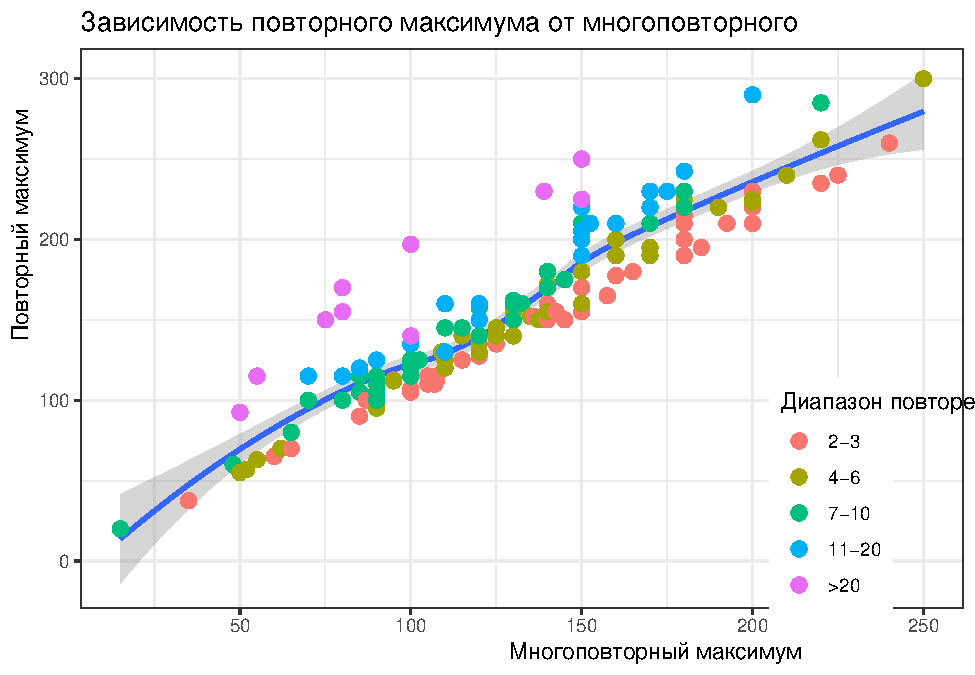
\includegraphics[width=0.85\linewidth]{Regression-model-for-estimating-RM_files/figure-latex/unnamed-chunk-20-1} \end{center}

Очевидно, что здесь будет близкая к линейной зависимость (учитывая
высокую корреляцию).

Оказывается, если предварительно разбить наблюдения на группы по
повторениями, линейность станет намного более выраженной для числа
повторений не больше 10 (для большего числа повторений не прослеживается
явной линейности либо из-за недостатка данных, либо по физиологическим
причинам, озвученным ранее; для диапазона 11-20 возможна квадратичная
зависимость, но мало данных, чтобы что-то подтвердить):

\begin{center}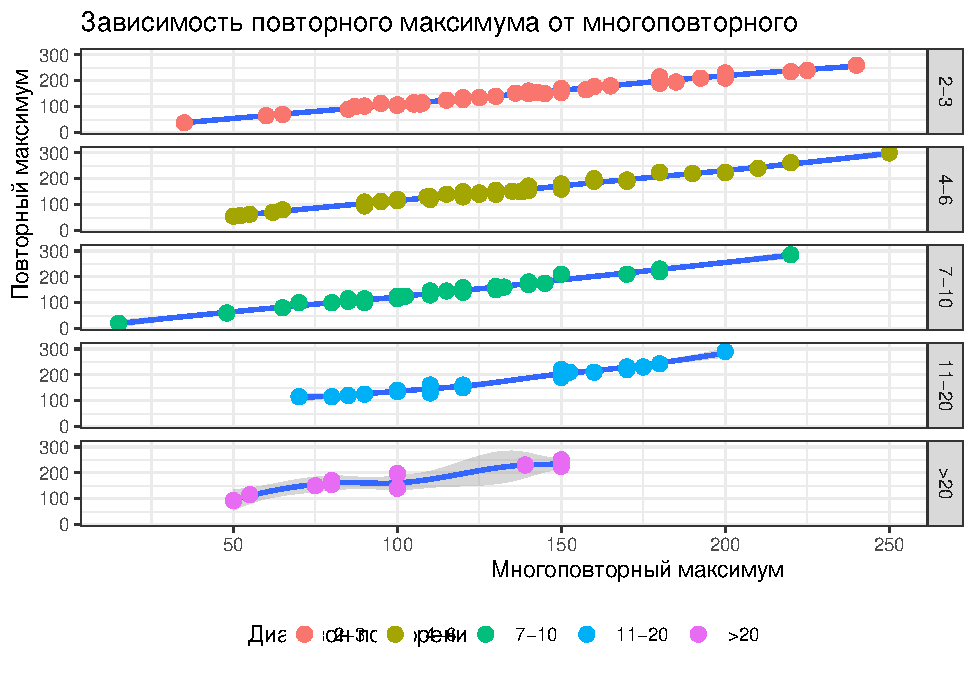
\includegraphics[width=0.9\linewidth]{Regression-model-for-estimating-RM_files/figure-latex/unnamed-chunk-21-1} \end{center}

Сказанное выше значит, что для каждого диапазона повторений нужен
отдельный анализ.

Есть ли зависимость между отношением \(\frac{RM}{MRM}\) в зависимости от
опыта тренировок и других факторов? Дисперсионный анализ показывает, что
нет:

\begin{Shaded}
\begin{Highlighting}[]
\CommentTok{# есть ли значимые различия в разных возрастных группах для фиксированного}
\CommentTok{# диапазона}

\KeywordTok{tibble}\NormalTok{(}\StringTok{`}\DataTypeTok{Диапозон повторений}\StringTok{`}\NormalTok{ =}\StringTok{ }\KeywordTok{levels}\NormalTok{(data}\OperatorTok{$}\NormalTok{CountGroup), Опыт =}\StringTok{ }\KeywordTok{sapply}\NormalTok{(}\KeywordTok{levels}\NormalTok{(data}\OperatorTok{$}\NormalTok{CountGroup), }
    \ControlFlowTok{function}\NormalTok{(x) }\KeywordTok{aov}\NormalTok{(RM}\OperatorTok{/}\NormalTok{MRM }\OperatorTok{~}\StringTok{ }\NormalTok{Experience, data }\OperatorTok\StringTok{ }\KeywordTok{filter}\NormalTok{(CountGroup }\OperatorTok{==}\StringTok{ }\NormalTok{x)) }\OperatorTok\StringTok{ }\KeywordTok{summary}\NormalTok{() }\OperatorTok\StringTok{ }
\StringTok{        }\NormalTok{.[[}\DecValTok{1}\NormalTok{]][[}\StringTok{"Pr(>F)"}\NormalTok{]][}\DecValTok{1}\NormalTok{]), Возраст =}\StringTok{ }\KeywordTok{sapply}\NormalTok{(}\KeywordTok{levels}\NormalTok{(data}\OperatorTok{$}\NormalTok{CountGroup), }\ControlFlowTok{function}\NormalTok{(x) }\KeywordTok{aov}\NormalTok{(RM}\OperatorTok{/}\NormalTok{MRM }\OperatorTok{~}\StringTok{ }
\StringTok{    }\NormalTok{AgeGroup, data }\OperatorTok\StringTok{ }\KeywordTok{filter}\NormalTok{(CountGroup }\OperatorTok{==}\StringTok{ }\NormalTok{x)) }\OperatorTok\StringTok{ }\KeywordTok{summary}\NormalTok{() }\OperatorTok\StringTok{ }\NormalTok{.[[}\DecValTok{1}\NormalTok{]][[}\StringTok{"Pr(>F)"}\NormalTok{]][}\DecValTok{1}\NormalTok{]), }
\NormalTok{    ИМТ =}\StringTok{ }\KeywordTok{sapply}\NormalTok{(}\KeywordTok{levels}\NormalTok{(data}\OperatorTok{$}\NormalTok{CountGroup), }\ControlFlowTok{function}\NormalTok{(x) }\KeywordTok{aov}\NormalTok{(RM}\OperatorTok{/}\NormalTok{MRM }\OperatorTok{~}\StringTok{ }\NormalTok{IndexGroup, data }\OperatorTok\StringTok{ }
\StringTok{        }\KeywordTok{filter}\NormalTok{(CountGroup }\OperatorTok{==}\StringTok{ }\NormalTok{x)) }\OperatorTok\StringTok{ }\KeywordTok{summary}\NormalTok{() }\OperatorTok\StringTok{ }\NormalTok{.[[}\DecValTok{1}\NormalTok{]][[}\StringTok{"Pr(>F)"}\NormalTok{]][}\DecValTok{1}\NormalTok{]), Телосложение =}\StringTok{ }\KeywordTok{sapply}\NormalTok{(}\KeywordTok{levels}\NormalTok{(data}\OperatorTok{$}\NormalTok{CountGroup), }
        \ControlFlowTok{function}\NormalTok{(x) }\KeywordTok{aov}\NormalTok{(RM}\OperatorTok{/}\NormalTok{MRM }\OperatorTok{~}\StringTok{ }\NormalTok{BodyType, data }\OperatorTok\StringTok{ }\KeywordTok{filter}\NormalTok{(CountGroup }\OperatorTok{==}\StringTok{ }\NormalTok{x)) }\OperatorTok\StringTok{ }
\StringTok{            }\KeywordTok{summary}\NormalTok{() }\OperatorTok\StringTok{ }\NormalTok{.[[}\DecValTok{1}\NormalTok{]][[}\StringTok{"Pr(>F)"}\NormalTok{]][}\DecValTok{1}\NormalTok{])) }\OperatorTok\StringTok{ }\KeywordTok{kable}\NormalTok{(}\DataTypeTok{caption =} \StringTok{"Значимость различий отношения ПМ к МПМ в каждом диапазоне повторений при разных уровнях факторных переменных"}\NormalTok{, }
    \DataTypeTok{align =} \StringTok{"ccccc"}\NormalTok{)}
\end{Highlighting}
\end{Shaded}

\begin{longtable}[]{@{}ccccc@{}}
\caption{Значимость различий отношения ПМ к МПМ в каждом диапазоне
повторений при разных уровнях факторных переменных}\tabularnewline
\toprule
Диапозон повторений & Опыт & Возраст & ИМТ & Телосложение\tabularnewline
\midrule
\endfirsthead
\toprule
Диапозон повторений & Опыт & Возраст & ИМТ & Телосложение\tabularnewline
\midrule
\endhead
2-3 & 0.6506219 & 0.7671962 & 0.5516303 & 0.7779869\tabularnewline
4-6 & 0.6178563 & 0.6907457 & 0.6655732 & 0.5432097\tabularnewline
7-10 & 0.1237067 & 0.8407336 & 0.8969795 & 0.3628399\tabularnewline
11-20 & 0.7293524 & 0.0354352 & 0.0304071 & 0.6845562\tabularnewline
\textgreater20 & 0.8249503 & 0.5901704 & 0.2511299 &
0.3736225\tabularnewline
\bottomrule
\end{longtable}

Единственное: обнаружилась разница в зависимости от возраста и индекса
массы тела для диапазона повторений 11-20. Возможно, это связано с тем,
что в целом с увеличением возраста увеличивается уровень подготовки,
отчего на более чем 10 раз удаётся поднимать больший процент от
максимального веса.

\begin{center}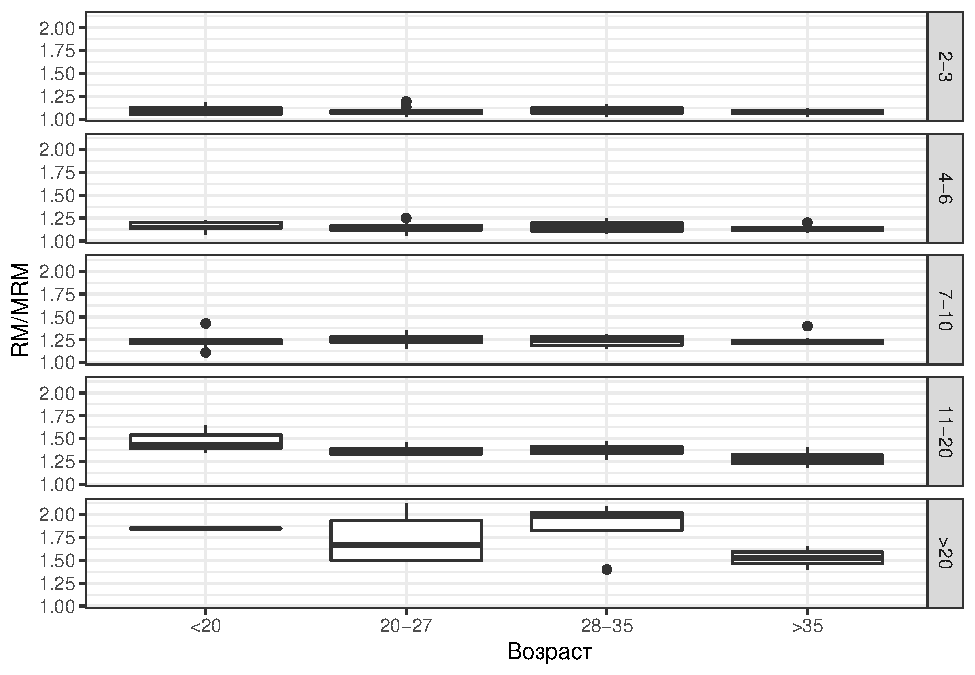
\includegraphics[width=0.9\linewidth]{Regression-model-for-estimating-RM_files/figure-latex/unnamed-chunk-23-1} \end{center}

Кроме того, \textbf{возможна разница между самими упражнениями}
(движениями):

\begin{Shaded}
\begin{Highlighting}[]
\CommentTok{# p-значения в зависимости от типа телосложения}

\NormalTok{(}\KeywordTok{sapply}\NormalTok{(}\KeywordTok{levels}\NormalTok{(data}\OperatorTok{$}\NormalTok{CountGroup), }\ControlFlowTok{function}\NormalTok{(x) }\KeywordTok{aov}\NormalTok{(RM}\OperatorTok{/}\NormalTok{MRM }\OperatorTok{~}\StringTok{ }\NormalTok{Action, data }\OperatorTok\StringTok{ }\KeywordTok{filter}\NormalTok{(CountGroup }\OperatorTok{==}\StringTok{ }
\StringTok{    }\NormalTok{x)) }\OperatorTok\StringTok{ }\KeywordTok{summary}\NormalTok{() }\OperatorTok\StringTok{ }\NormalTok{.[[}\DecValTok{1}\NormalTok{]][[}\StringTok{"Pr(>F)"}\NormalTok{]][}\DecValTok{1}\NormalTok{])) }\OperatorTok\StringTok{ }\KeywordTok{pander}\NormalTok{()}
\end{Highlighting}
\end{Shaded}

\begin{longtable}[]{@{}ccccc@{}}
\toprule
\begin{minipage}[b]{0.12\columnwidth}\centering
2-3\strut
\end{minipage} & \begin{minipage}[b]{0.11\columnwidth}\centering
4-6\strut
\end{minipage} & \begin{minipage}[b]{0.13\columnwidth}\centering
7-10\strut
\end{minipage} & \begin{minipage}[b]{0.11\columnwidth}\centering
11-20\strut
\end{minipage} & \begin{minipage}[b]{0.11\columnwidth}\centering
\textgreater20\strut
\end{minipage}\tabularnewline
\midrule
\endhead
\begin{minipage}[t]{0.12\columnwidth}\centering
0.06367\strut
\end{minipage} & \begin{minipage}[t]{0.11\columnwidth}\centering
0.2752\strut
\end{minipage} & \begin{minipage}[t]{0.13\columnwidth}\centering
0.006814\strut
\end{minipage} & \begin{minipage}[t]{0.11\columnwidth}\centering
0.7637\strut
\end{minipage} & \begin{minipage}[t]{0.11\columnwidth}\centering
0.1085\strut
\end{minipage}\tabularnewline
\bottomrule
\end{longtable}

\begin{Shaded}
\begin{Highlighting}[]
\KeywordTok{ggplot}\NormalTok{(data }\OperatorTok\StringTok{ }\KeywordTok{filter}\NormalTok{(Count }\OperatorTok{<=}\StringTok{ }\DecValTok{20}\NormalTok{), }\KeywordTok{aes}\NormalTok{(}\DataTypeTok{x =}\NormalTok{ Action, }\DataTypeTok{y =}\NormalTok{ RM}\OperatorTok{/}\NormalTok{MRM)) }\OperatorTok{+}\StringTok{ }\KeywordTok{geom_boxplot}\NormalTok{() }\OperatorTok{+}\StringTok{ }
\StringTok{    }\KeywordTok{facet_grid}\NormalTok{(}\KeywordTok{vars}\NormalTok{(CountGroup)) }\OperatorTok{+}\StringTok{ }\KeywordTok{theme_bw}\NormalTok{() }\OperatorTok{+}\StringTok{ }\KeywordTok{labs}\NormalTok{(}\DataTypeTok{x =} \StringTok{"Движение"}\NormalTok{) }\OperatorTok{+}\StringTok{ }\KeywordTok{coord_flip}\NormalTok{()}
\end{Highlighting}
\end{Shaded}

\begin{center}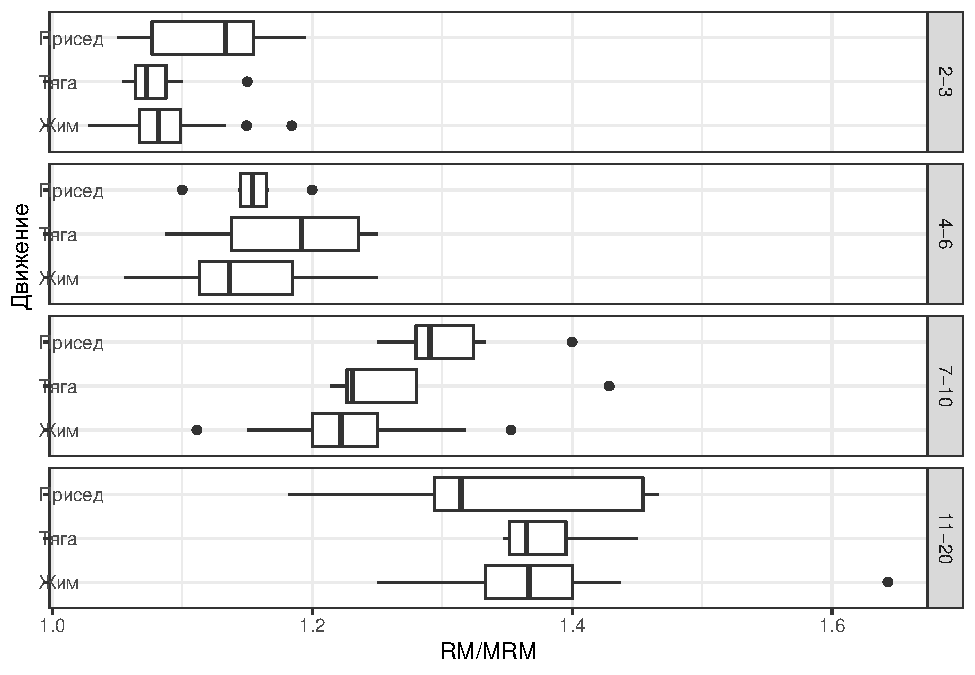
\includegraphics[width=0.9\linewidth]{Regression-model-for-estimating-RM_files/figure-latex/unnamed-chunk-24-1} \end{center}

Дополнительные закономерности:

\begin{center}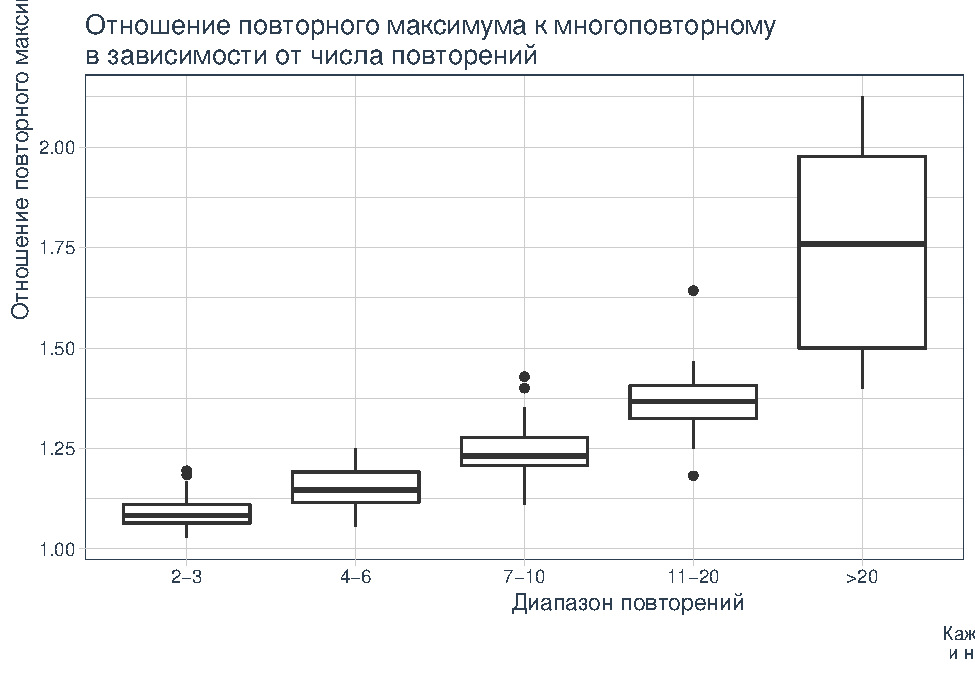
\includegraphics[width=0.85\linewidth]{Regression-model-for-estimating-RM_files/figure-latex/unnamed-chunk-25-1} \end{center}

\begin{center}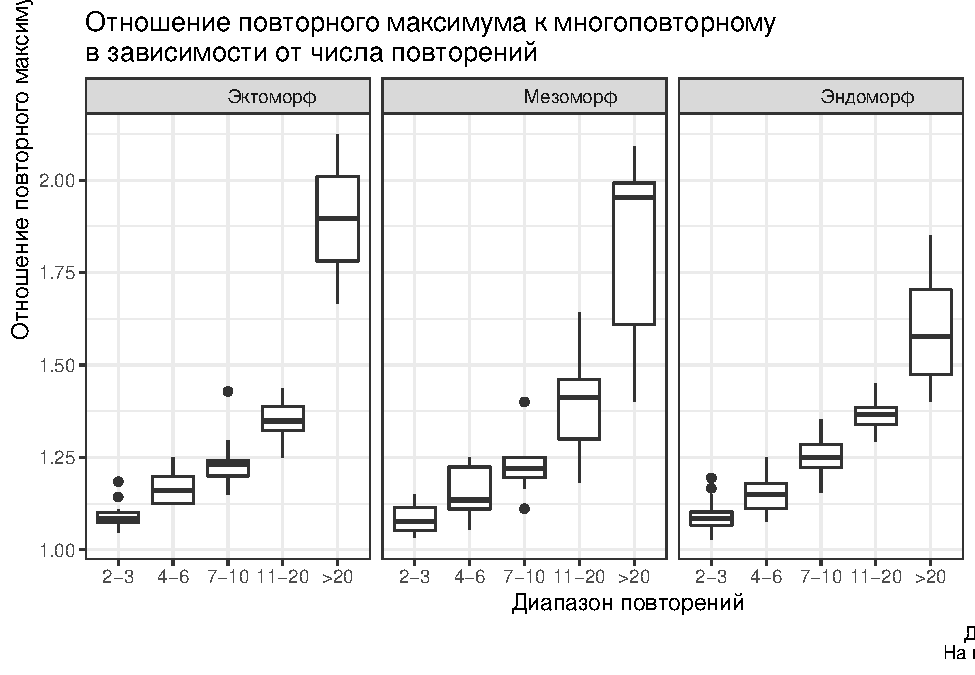
\includegraphics[width=0.85\linewidth]{Regression-model-for-estimating-RM_files/figure-latex/unnamed-chunk-25-2} \end{center}

\begin{center}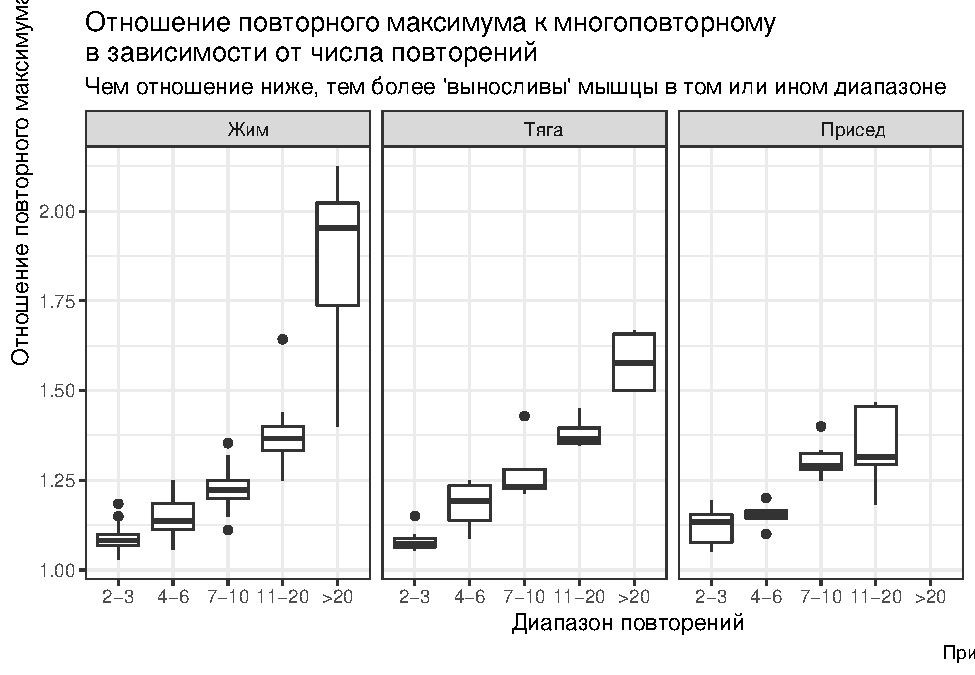
\includegraphics[width=0.85\linewidth]{Regression-model-for-estimating-RM_files/figure-latex/unnamed-chunk-25-3} \end{center}

\hypertarget{ux438ux441ux43fux440ux430ux432ux43bux435ux43dux438ux435-ux43eux43fux435ux447ux430ux442ux43eux43a}{%
\subsection{Исправление
опечаток}\label{ux438ux441ux43fux440ux430ux432ux43bux435ux43dux438ux435-ux43eux43fux435ux447ux430ux442ux43eux43a}}

Часто при сборе данных возникают \emph{ненормальные} наблюдения,
полученные из-за опечаток или недопониманий. В этот раз таких наблюдений
накопилось около 10\%. Если поразмыслить над их причинностью, то чаще
всего испытуемый забывал поставить цифру ``1'' перед числом, в
результате вместо роста 175 получался рост 75 и т. п.

В то же время могло быть и так, что испытуемый неверно понял суть
исследования и в анкете описывал просто подход, который был выполнен, а
не подход для многоповторного максимума (то есть на пределе усилий),
либо при проходке использовал экипировку или другую технику упражнения,
либо, опять же, опечатался; в итоге жим 170х5 оказывался равным 220,
хотя ясно, что тут должны стоять 170х5 и 200 либо 170х15 и 220.

С такими \emph{выбросами} можно сделать только две вещи:

\begin{enumerate}
\def\labelenumi{\arabic{enumi}.}
\tightlist
\item
  исправить их, опираясь на логику либо переспросить того, кому это
  наблюдение принадлежит\footnote{к сожалению, этого не получилось
    сделать, так как испытуемые редко пользуются электронной почтой,
    видимо};
\item
  удалить из выборки.
\end{enumerate}

В итоге некоторые данные были исправлены на более вероятный вариант, а
явные непонятные аномалии были удалены из выборки.
\href{https://github.com/PasaOpasen/Powerlifting-training-diary-and-articles/blob/master/Estimating\%20RM/data.tsv}{В
файле с исходными данными} содержатся комментарии, где и что я исправил
и почему.

\hypertarget{ux443ux434ux430ux43bux451ux43dux43dux44bux435-ux434ux430ux43dux43dux44bux435}{%
\subsection{Удалённые
данные}\label{ux443ux434ux430ux43bux451ux43dux43dux44bux435-ux434ux430ux43dux43dux44bux435}}

Перед построением модели из обучающей выборки заранее \textbf{были
исключены следующие наблюдения}:

\begin{itemize}
\item
  некоторые \textbf{выбросы}, в том числе несколько наблюдений, которые
  изначально не вписывались в модель и по логике очень сомнительны; речь
  идёт о наблюдениях типа \(120*3=140\), хотя интуитивно понятно, что
  140 -- это как минимум 120 на 5; возможно, подход 120 на 3 был сделан
  в достаточно отдалённый от проходки период либо во время проходки в
  качестве разминочного, то есть его нельзя считать многоповторным
  максимумом, эквивалентным повторному максимуму; конечно, здесь может
  играть роль какой-то особый случай\footnote{например, высокий импульс
    ЦНС, не соответствующий уровню креатинфосфата. В таком случае
    человек может на раз пожать большой вес, но на несколько раз уже
    \emph{недостаточно большой}: при ПМ в 140 на 3 раза жмётся не почти
    130, а 120}, который является выбросом (потому должен быть исключён)
  либо не может быть выявлен по тому набору признаков, которые доступны
  в нашем случае;
\item
  \textbf{наблюдения с числом повторений больше 20}, так как сама идея
  предсказать 1ПМ по, например, 30ПМ -- абсурдна, поскольку здесь имеют
  место в корне разные нагрузки, задействуются разные типы мышечных
  волокон и имеет место разный энергетический обмен; по этой причине
  использование таких данных при создании моделей приводит к искажениям,
  а для самих этих наблюдений модель предсказывает лишь какую-то нижнюю
  границу 1ПМ, в чём нет смысла\footnote{такую нижнюю границу можно
    предсказать, просто умножив вес примерно на 1.5, исследование же
    рассчитано на поиск верхней границы}; вдобавок, для таких
  предсказаний сложнее определить аномальные наблюдения в смысле
  предыдущего пункта; кроме того, даже на графиках видно, что диапазон
  выше 20 очень сильно отличается от остальных диапазонов.
\end{itemize}

Как итог, теперь для данных верны следующие статистики:

\begin{verbatim}
##        RM             MRM          Count           Action         Sex     
##  Min.   : 20.0   Min.   : 15   Min.   : 2.000   Жим   :116   Мужчина:153  
##  1st Qu.:120.0   1st Qu.:100   1st Qu.: 3.000   Тяга  : 22   Женщина:  9  
##  Median :145.0   Median :125   Median : 5.000   Присед: 24                
##  Mean   :152.6   Mean   :129   Mean   : 6.636                             
##  3rd Qu.:190.0   3rd Qu.:150   3rd Qu.: 9.000                             
##  Max.   :300.0   Max.   :250   Max.   :20.000                             
##                                                                           
##          Experience      Age         Weight           Height        BodyType 
##  До двух лет  :31   Min.   :15   Min.   : 47.00   Min.   :155   Эктоморф:34  
##  2-3 года     :28   1st Qu.:21   1st Qu.: 78.00   1st Qu.:170   Мезоморф:46  
##  4-5 лет      :45   Median :27   Median : 87.00   Median :177   Эндоморф:82  
##  6-10 лет     :32   Mean   :28   Mean   : 89.59   Mean   :177                
##  больше 10 лет:26   3rd Qu.:33   3rd Qu.:102.75   3rd Qu.:183                
##                     Max.   :62   Max.   :160.00   Max.   :198                
##                                                                              
##  CountGroup  AgeGroup      Index                    IndexGroup
##  2-3  :47   <20  :30   Min.   :18.83   выраженный дефицит: 0  
##  4-6  :51   20-27:55   1st Qu.:25.17   дефицит           : 0  
##  7-10 :41   28-35:50   Median :27.76   норма             :36  
##  11-20:23   >35  :27   Mean   :28.44   избыток           :66  
##  >20  : 0              3rd Qu.:31.39   ожирение1         :42  
##                        Max.   :45.27   ожирение2         :12  
##                                        ожирение3         : 6
\end{verbatim}

\begin{center}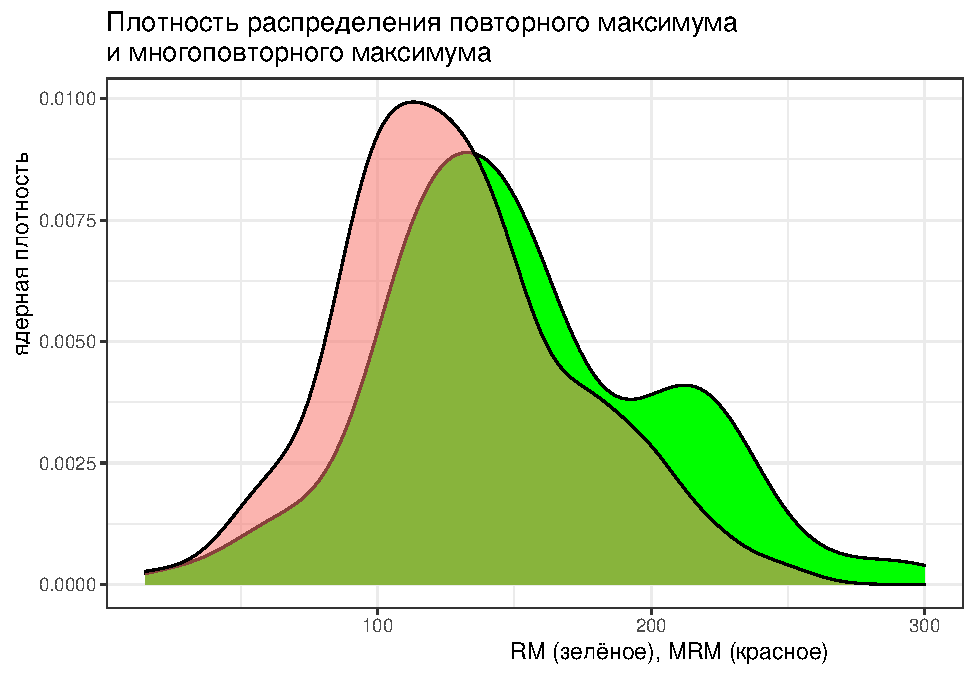
\includegraphics[width=0.85\linewidth]{Regression-model-for-estimating-RM_files/figure-latex/unnamed-chunk-26-1} \end{center}

\begin{center}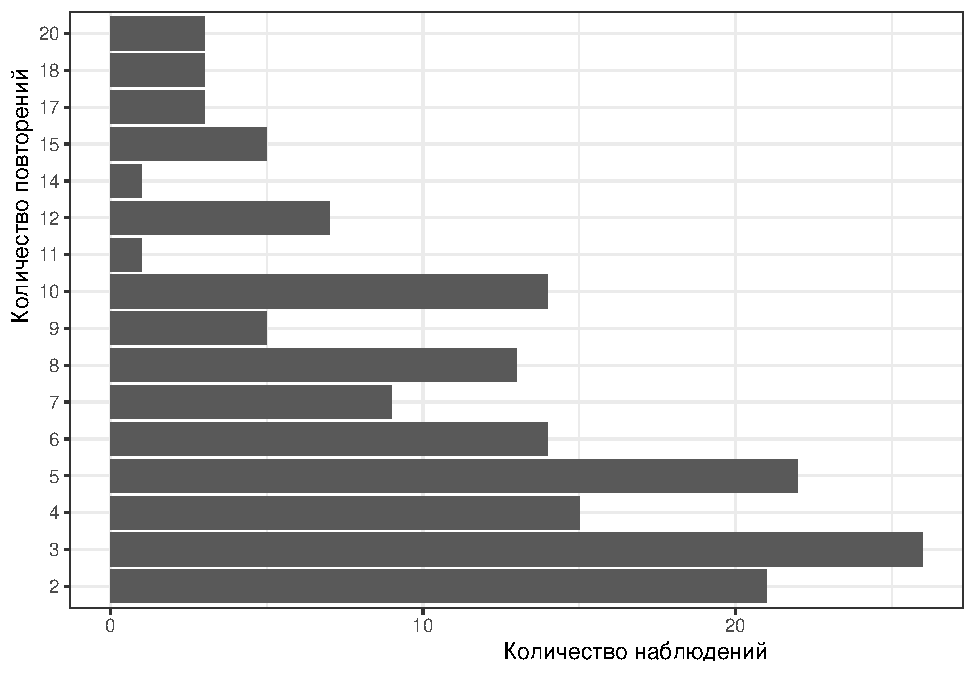
\includegraphics[width=0.85\linewidth]{Regression-model-for-estimating-RM_files/figure-latex/unnamed-chunk-26-2} \end{center}

\begin{center}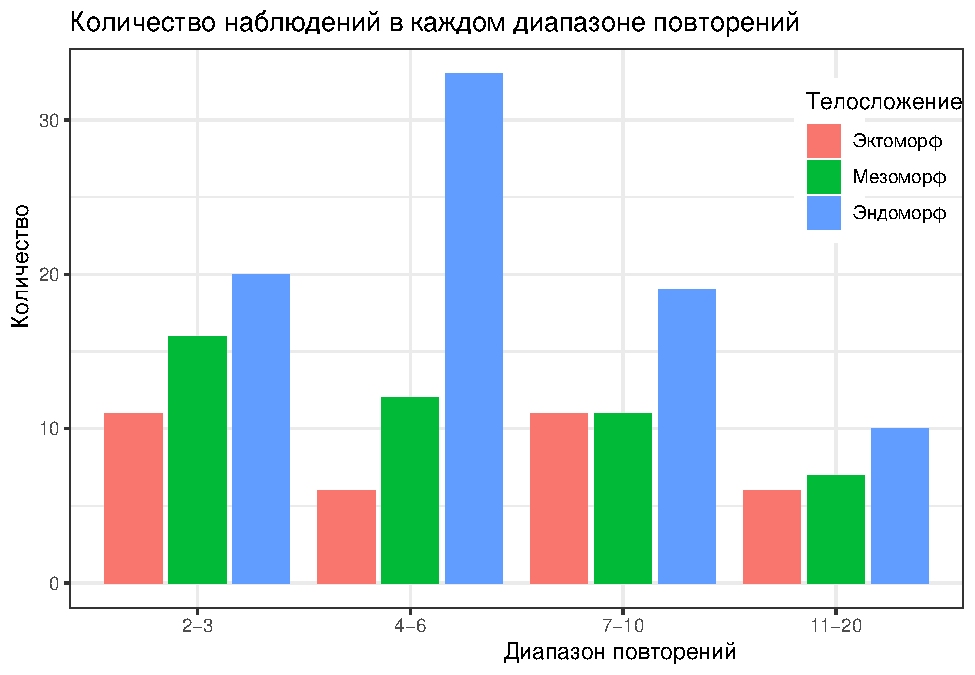
\includegraphics[width=0.85\linewidth]{Regression-model-for-estimating-RM_files/figure-latex/unnamed-chunk-26-3} \end{center}

\begin{center}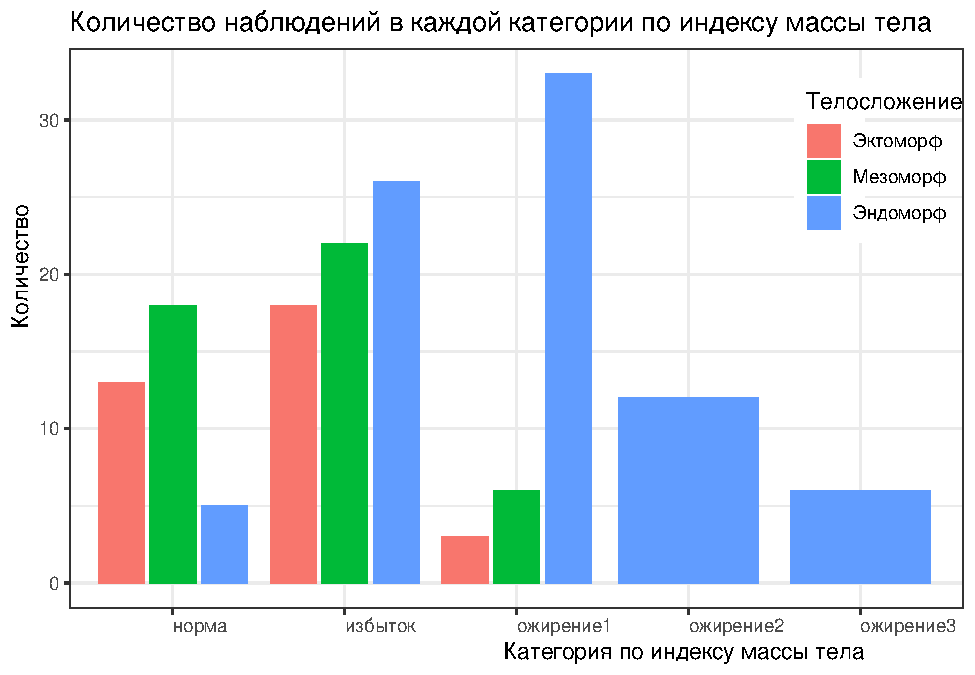
\includegraphics[width=0.85\linewidth]{Regression-model-for-estimating-RM_files/figure-latex/unnamed-chunk-26-4} \end{center}

\begin{center}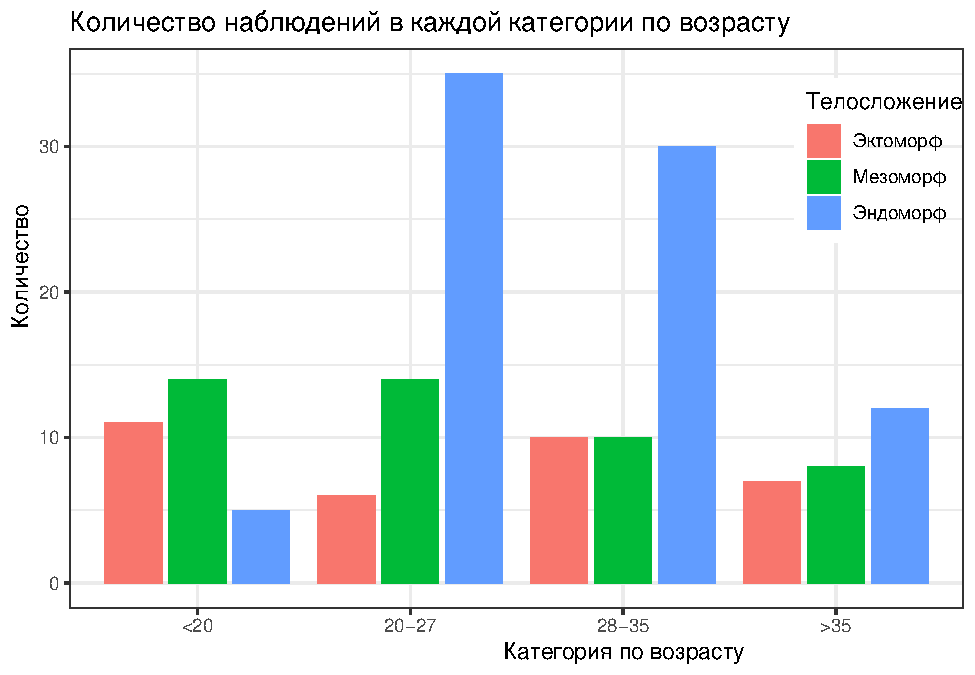
\includegraphics[width=0.85\linewidth]{Regression-model-for-estimating-RM_files/figure-latex/unnamed-chunk-26-5} \end{center}

\begin{center}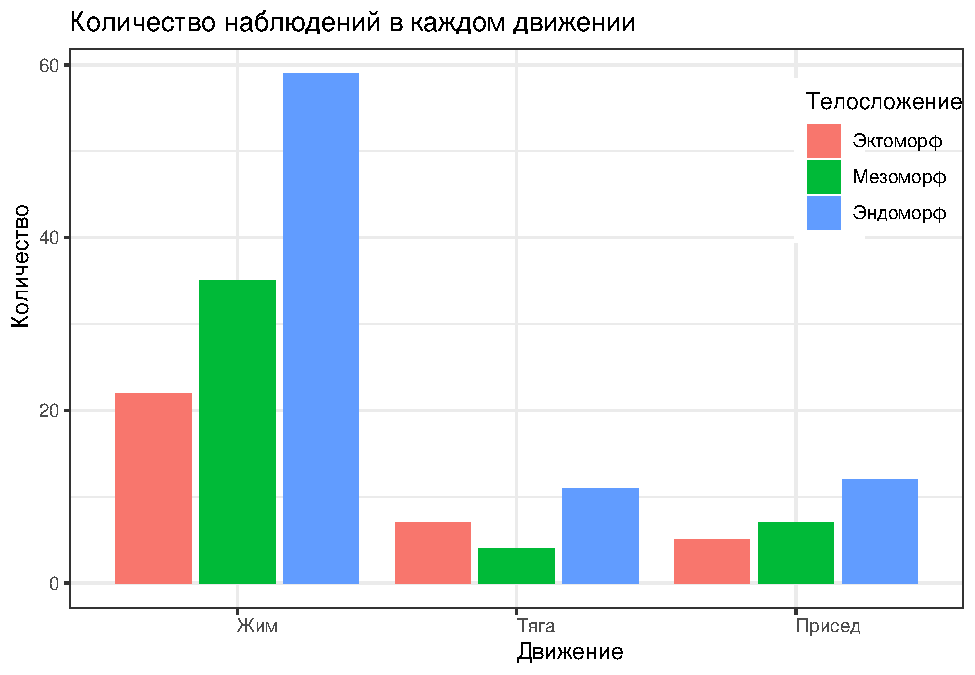
\includegraphics[width=0.85\linewidth]{Regression-model-for-estimating-RM_files/figure-latex/unnamed-chunk-26-6} \end{center}

\begin{center}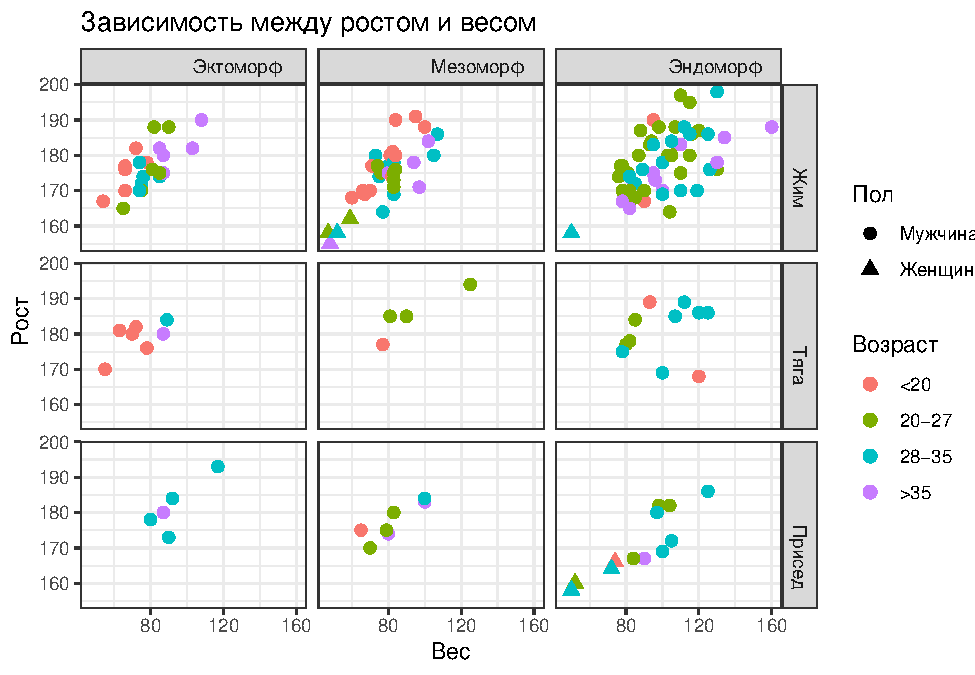
\includegraphics[width=0.85\linewidth]{Regression-model-for-estimating-RM_files/figure-latex/unnamed-chunk-26-7} \end{center}

\hypertarget{ux43fux43eux434ux432ux435ux434ux435ux43dux438ux435-ux438ux442ux43eux433ux43eux432-ux438-ux43eux442ux431ux43eux440-ux43fux440ux438ux437ux43dux430ux43aux43eux432}{%
\subsection{Подведение итогов и отбор
признаков}\label{ux43fux43eux434ux432ux435ux434ux435ux43dux438ux435-ux438ux442ux43eux433ux43eux432-ux438-ux43eux442ux431ux43eux440-ux43fux440ux438ux437ux43dux430ux43aux43eux432}}

Перечислим основные идеи об особенностях данных, сказанные ранее:

\begin{itemize}
\item
  Любые \textbf{полученные результаты не следует обобщать на женщин},
  так как в опросе они почти не участвовали. Возможно, ради точности
  вычислений даже придётся убрать женщин из выборки;
\item
  \textbf{Эндоморфы среди пауэрлифтеров встречаются чаще мезоморфов или
  эктоморфов. При этом у эндоморфов значимо чаще встречается ``ожирение
  первой стадии'', чем у представителей других телосложений};
\item
  \textbf{Результаты в приседе растут с увеличением индекса массы тела
  лишь до некоторого порога}. Увеличение индекса массы тела выше
  ``ожирения первой стадии'' не будет полезным;
\item
  \textbf{Сильная корреляция между индексом массы тела и повторным
  максимумом наблюдается у мезофорфов -- в жиме, у эктоморфов -- в тяге,
  у эндоморфов -- в приседе};
\item
  Не обнаружено значимой разницы значений \(\frac{MRM}{RM}\) для разных
  телосложений, движений, групп по индексу массы, опыта, возраста для
  любого конкретного числа повторений или диапазона повторений (но при
  этом обнаружилась разница между движениями для диапазонов повторений
  до 10); \textbf{процентовки от \emph{National Strength and
  Conditioning Association (NSCA)} с небольшими погрешностями верны для
  всех спортсменов и всех движений};
\item
  \textbf{Разбиение наблюдений на группы по диапазону повторений
  (который сделан согласовано с физиологическими соображениями) должно
  значительно повысить точность модели}, причем для числа повторений до
  10-20 эта модель крайне близка к линейной;
\item
  Наблюдения свыше 20 повторений не будут учитываться, так как их мало и
  этот диапазон слабо коррелирует с абсолютной силой;
\item
  \textbf{При более чем 10 повторений опытные спортсмены способны
  поднимать более близкие к максимальным веса, чем неопытные}.
\end{itemize}

Соображения о предикторах для модели:

\begin{itemize}
\item
  \(RM\) (повторный максимум) обязательно зависит как от \(MRM\)
  (многоповторный максимум) и \(Count\) (числа повторений), так и от
  \(CountGroup\) -- группы по числу повторений;
\item
  \(RM\) может зависеть также от \(BodyType\) (типа телосложения) и
  \(Action\) (упражнения) либо от их бинарных модификаций (например,
  если людей разделить не на 3 телосложения, а на эндоморфов и не
  эндоморфов); возможно, стоит также попробовать учесть индекс массы
  тела или собственно вес, имеющие корреляцию с \(RM\) не меньше 0.5.
\end{itemize}

Дальнейшие действия:

\begin{enumerate}
\def\labelenumi{\arabic{enumi}.}
\item
  Просмотреть, как работает модель Вендлера, и на её примере
  ознакомиться с шаблоном по оценке качества, который будет
  использоваться для оценки следующих моделей.
\item
  Построить разные модели для оценки конкретно \(RM\) и выбрать ту,
  которая более проста и даёт меньшую ошибку кросс-валидации.
\item
  Сравнить выбранные модели и определить лучшую из них.
\end{enumerate}

\begin{center}\rule{0.5\linewidth}{0.5pt}\end{center}

\hypertarget{ux43fux43eux441ux442ux440ux43eux435ux43dux438ux435-ux43cux43eux434ux435ux43bux435ux439}{%
\section{Построение
моделей}\label{ux43fux43eux441ux442ux440ux43eux435ux43dux438ux435-ux43cux43eux434ux435ux43bux435ux439}}

Вычислительные возможности позволяют создать и проверить огромное
количество моделей. Цель исследователя -- предложить несколько вариантов
и выбрать среди них лучший. Кроме этого, нужно посмотреть, как работает
модель на разных группах данных, чтобы обнаружить выбросы или
обнаружить, что на такой-то группе модель вообще не может работать,
из-за чего такую группу придётся исключить (эта работа уже проделана при
самом исследовании, чтобы не нагружать статью).

Итак, в модели представляют интерес следующие показатели:

\begin{itemize}
\item
  ошибки в разных группах данных;
\item
  выбросы и влиятельные наблюдения;
\item
  статистическая значимость модели и её составляющих;
\item
  оценки кросс-валидации.
\end{itemize}

\hypertarget{ux43dux435ux434ux43eux441ux442ux430ux442ux43aux438-ux438ux441ux445ux43eux434ux43dux43eux433ux43e-ux440ux435ux448ux435ux43dux438ux44f}{%
\subsection{Недостатки исходного
решения}\label{ux43dux435ux434ux43eux441ux442ux430ux442ux43aux438-ux438ux441ux445ux43eux434ux43dux43eux433ux43e-ux440ux435ux448ux435ux43dux438ux44f}}

Применив формулу \(RM=MRM \cdot(1+0.0333 \cdot Count)\) ко всем
наблюдениям, получим оценки \(RM\) (Fact), которые будут отличаться от
истинного \(RM\) (Target). Разница между этими величинами -- остатки.
Для модели Вендлера остатки будут следующие:

\begin{center}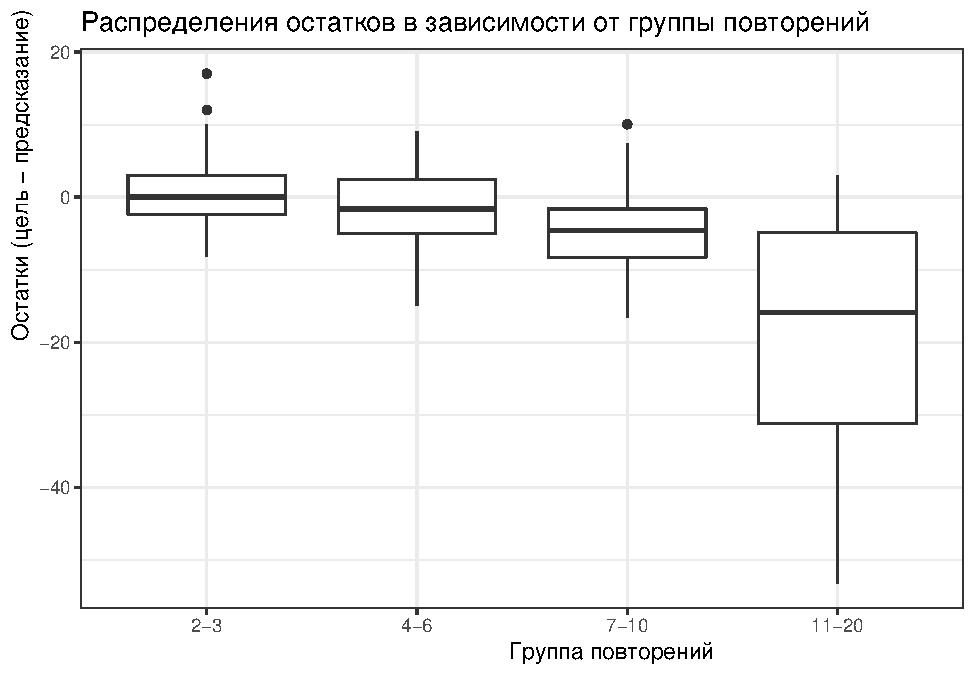
\includegraphics{Regression-model-for-estimating-RM_files/figure-latex/unnamed-chunk-28-1} \end{center}

\begin{center}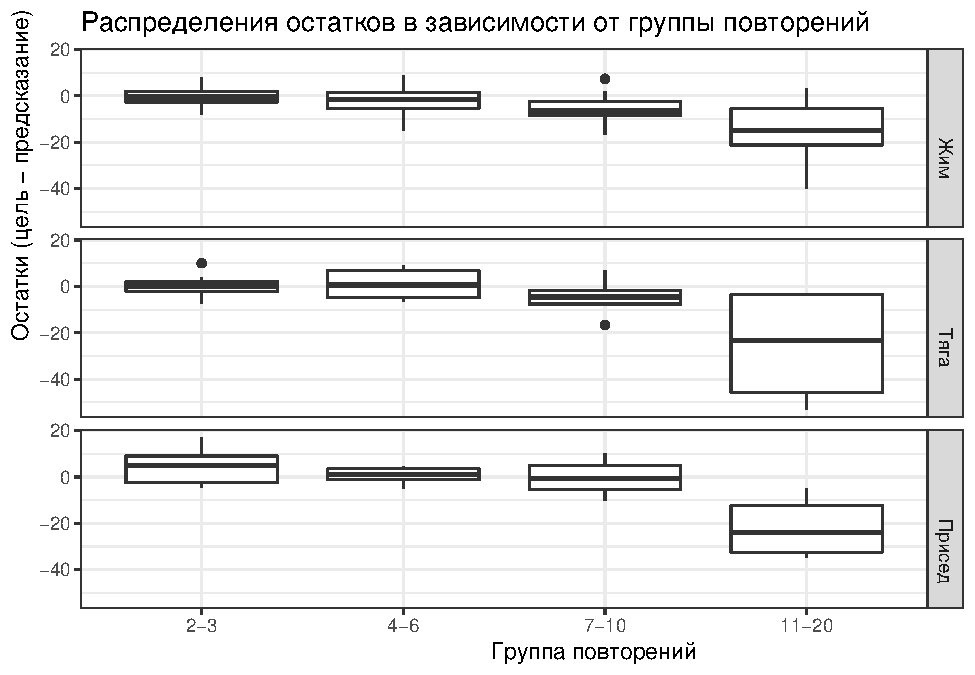
\includegraphics{Regression-model-for-estimating-RM_files/figure-latex/unnamed-chunk-28-2} \end{center}

\begin{center}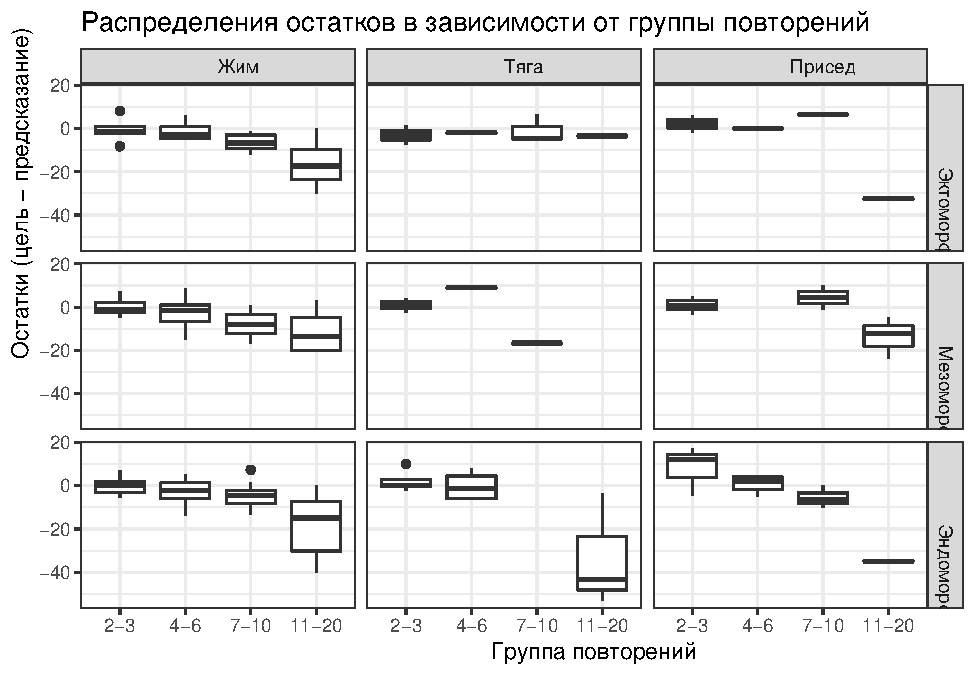
\includegraphics{Regression-model-for-estimating-RM_files/figure-latex/unnamed-chunk-28-3} \end{center}

Здесь такая логика: чем лучше модель, тем ``ящики'' тоньше и тем их
середины ближе к 0.

В данном случае видно, что \textbf{модель Вендлера хорошо работает почти
на всех данных из диапазона 2-3 и на немалой части данных из диапазона
4-6}. Для большего числа повторений модель даёт завышенные оценки.

Если посмотреть на численные ошибки

\begin{verbatim}
## Ошибки модели (выведены 15 элементов с наибольшими ошибками): 
## 
## 
## | Fact| Target|   ERROR| ErrorPercent| MRM| Count|Action |Sex     | Weight|CountGroup |    Index|
## |----:|------:|-------:|------------:|---:|-----:|:------|:-------|------:|:----------|--------:|
## |  283|    230| 53.2200|    23.139130| 170|    20|Тяга   |Мужчина |     82|11-20      | 25.88057|
## |  333|    290| 43.2000|    14.896552| 200|    20|Тяга   |Мужчина |    107|11-20      | 31.26370|
## |  200|    160| 39.9200|    24.950000| 120|    20|Жим    |Мужчина |    115|11-20      | 30.24326|
## |  255|    220| 34.9150|    15.870454| 170|    15|Присед |Мужчина |     90|11-20      | 32.27079|
## |  240|    205| 34.9100|    17.029268| 150|    18|Жим    |Мужчина |    110|11-20      | 38.06228|
## |  262|    230| 32.4125|    14.092391| 175|    15|Присед |Мужчина |     92|11-20      | 27.17391|
## |  180|    150| 29.9400|    19.960000| 120|    15|Жим    |Мужчина |     87|11-20      | 28.40816|
## |  154|    130| 23.9560|    18.427692| 110|    12|Присед |Мужчина |     80|11-20      | 26.42357|
## |  157|    135| 21.6100|    16.007407| 100|    17|Жим    |Мужчина |     75|11-20      | 25.35154|
## |  210|    190| 19.9400|    10.494737| 150|    12|Жим    |Мужчина |    105|11-20      | 32.40741|
## |  220|    200| 19.9300|     9.965000| 150|    14|Жим    |Мужчина |     83|11-20      | 28.38480|
## |  198|    215| 17.0180|     7.915349| 180|     3|Присед |Мужчина |     84|2-3        | 30.11940|
## |  147|    130| 16.6300|    12.792308| 110|    10|Жим    |Мужчина |    100|7-10       | 28.29335|
## |  187|    170| 16.6200|     9.776471| 140|    10|Тяга   |Мужчина |     77|7-10       | 24.57787|
## |  156|    140| 15.9640|    11.402857| 120|     9|Жим    |Мужчина |     77|7-10       | 28.62879|
## 
## ------------> Наибольшая ошибка в большую сторону: 53.22 
## ------------> Наибольшая ошибка в меньшую сторону: 17.018 
## Модель ошиблась более чем на 5 % в 48 случаях из 162 ( 29.62963 %)
## Модель ошиблась более чем на 5 кг в 69 случаях из 162 ( 42.59259 %)
## ----------------> Статистика по ошибкам в процентах:
##      Min.   1st Qu.    Median      Mean   3rd Qu.      Max. 
##  0.009091  1.466058  2.895000  4.466610  6.231771 24.950000 
## -------------------> Среднеквадратичная ошибка: 10.79902
\end{verbatim}

увидим, что модель заметно ошибается в 30\% случаев и в среднем на почти
5\%. Первые формулы
\href{https://power-fitness.ru/metod-morisa-i-rajdina-ili-kak-uznat-svoj-maksimum-v-zhime-lezha.html}{Мориса
и Райдина} показывают худший результат:

\begin{verbatim}
## Ошибки модели (выведены 15 элементов с наибольшими ошибками): 
## 
## 
## | Fact| Target|    ERROR| ErrorPercent|   MRM| Count|Action |Sex     | Weight|CountGroup |    Index|
## |----:|------:|--------:|------------:|-----:|-----:|:------|:-------|------:|:----------|--------:|
## |  214|  160.0| 54.49607|    34.060045| 120.0|    20|Жим    |Мужчина |    115|11-20      | 30.24326|
## |  252|  205.0| 47.21174|    23.030117| 150.0|    18|Жим    |Мужчина |    110|11-20      | 38.06228|
## |  245|  285.0| 40.32727|    14.149919| 220.0|     8|Присед |Мужчина |     90|7-10       | 30.07117|
## |  172|  210.0| 38.08000|    18.133332| 150.0|    10|Присед |Мужчина |    100|7-10       | 29.86055|
## |  185|  220.0| 34.64382|    15.747191| 150.0|    15|Присед |Мужчина |    100|11-20      | 29.53686|
## |  184|  150.0| 34.08110|    22.720734| 120.0|    15|Жим    |Мужчина |     87|11-20      | 28.40816|
## |  209|  242.5| 33.06764|    13.636140| 180.0|    11|Тяга   |Мужчина |     78|11-20      | 25.18079|
## |  194|  225.0| 30.74906|    13.666249| 180.0|     6|Тяга   |Мужчина |     90|4-6        | 26.29657|
## |  270|  300.0| 30.20703|    10.069009| 250.0|     6|Присед |Мужчина |    117|4-6        | 31.41024|
## |  180|  210.0| 29.87365|    14.225546| 152.5|    12|Тяга   |Мужчина |     85|11-20      | 25.10633|
## |  186|  215.0| 29.32444|    13.639276| 180.0|     3|Присед |Мужчина |     84|2-3        | 30.11940|
## |  163|  135.0| 28.07674|    20.797583| 100.0|    17|Жим    |Мужчина |     75|11-20      | 25.35154|
## |  173|  200.0| 27.33250|    13.666249| 160.0|     6|Тяга   |Мужчина |    120|4-6        | 34.68609|
## |  237|  262.0| 24.58218|     9.382513| 220.0|     6|Тяга   |Мужчина |     89|4-6        | 26.28781|
## |  186|  210.0| 24.32444|    11.583069| 180.0|     3|Присед |Мужчина |    125|2-3        | 36.13134|
## 
## ------------> Наибольшая ошибка в большую сторону: 54.49607 
## ------------> Наибольшая ошибка в меньшую сторону: 40.32727 
## Модель ошиблась более чем на 5 % в 71 случаях из 162 ( 43.82716 %)
## Модель ошиблась более чем на 5 кг в 92 случаях из 162 ( 56.79012 %)
## ----------------> Статистика по ошибкам в процентах:
##     Min.  1st Qu.   Median     Mean  3rd Qu.     Max. 
##  0.03358  1.89439  4.28278  5.81013  8.61114 34.06004 
## -------------------> Среднеквадратичная ошибка: 13.73176
\end{verbatim}

На самом деле это две формулы вида

\[\log \left(\frac{RM}{MRM}\right)= a+b \cdot Count,\]

где \(a,b\) зависят от того, к какой части тела относится упражнение.
Сама идея сделать логарифмическое преобразование используется нередко,
но здесь это имеет негативный эффект: \(R^2\) равен далеко не 0.99, как
сказано на сайте (где я нашёл эти формулы):

\begin{longtable}[]{@{}ccccc@{}}
\toprule
\begin{minipage}[b]{0.29\columnwidth}\centering
~\strut
\end{minipage} & \begin{minipage}[b]{0.13\columnwidth}\centering
Estimate\strut
\end{minipage} & \begin{minipage}[b]{0.16\columnwidth}\centering
Std. Error\strut
\end{minipage} & \begin{minipage}[b]{0.12\columnwidth}\centering
t value\strut
\end{minipage} & \begin{minipage}[b]{0.14\columnwidth}\centering
Pr(\textgreater\textbar t\textbar)\strut
\end{minipage}\tabularnewline
\midrule
\endhead
\begin{minipage}[t]{0.29\columnwidth}\centering
\textbf{(Intercept)}\strut
\end{minipage} & \begin{minipage}[t]{0.13\columnwidth}\centering
0.06472\strut
\end{minipage} & \begin{minipage}[t]{0.16\columnwidth}\centering
0.01162\strut
\end{minipage} & \begin{minipage}[t]{0.12\columnwidth}\centering
5.57\strut
\end{minipage} & \begin{minipage}[t]{0.14\columnwidth}\centering
1.071e-07\strut
\end{minipage}\tabularnewline
\begin{minipage}[t]{0.29\columnwidth}\centering
\textbf{Action2Up}\strut
\end{minipage} & \begin{minipage}[t]{0.13\columnwidth}\centering
-0.02185\strut
\end{minipage} & \begin{minipage}[t]{0.16\columnwidth}\centering
0.01395\strut
\end{minipage} & \begin{minipage}[t]{0.12\columnwidth}\centering
-1.567\strut
\end{minipage} & \begin{minipage}[t]{0.14\columnwidth}\centering
0.1191\strut
\end{minipage}\tabularnewline
\begin{minipage}[t]{0.29\columnwidth}\centering
\textbf{Action2Down:Count}\strut
\end{minipage} & \begin{minipage}[t]{0.13\columnwidth}\centering
0.01701\strut
\end{minipage} & \begin{minipage}[t]{0.16\columnwidth}\centering
0.001341\strut
\end{minipage} & \begin{minipage}[t]{0.12\columnwidth}\centering
12.69\strut
\end{minipage} & \begin{minipage}[t]{0.14\columnwidth}\centering
7.031e-26\strut
\end{minipage}\tabularnewline
\begin{minipage}[t]{0.29\columnwidth}\centering
\textbf{Action2Up:Count}\strut
\end{minipage} & \begin{minipage}[t]{0.13\columnwidth}\centering
0.01823\strut
\end{minipage} & \begin{minipage}[t]{0.16\columnwidth}\centering
0.001013\strut
\end{minipage} & \begin{minipage}[t]{0.12\columnwidth}\centering
17.99\strut
\end{minipage} & \begin{minipage}[t]{0.14\columnwidth}\centering
4.325e-40\strut
\end{minipage}\tabularnewline
\bottomrule
\end{longtable}

\begin{longtable}[]{@{}cccc@{}}
\caption{Fitting linear model: log(RM/MRM) \textasciitilde{} Action2 +
Count:Action2}\tabularnewline
\toprule
\begin{minipage}[b]{0.18\columnwidth}\centering
Observations\strut
\end{minipage} & \begin{minipage}[b]{0.27\columnwidth}\centering
Residual Std. Error\strut
\end{minipage} & \begin{minipage}[b]{0.11\columnwidth}\centering
\(R^2\)\strut
\end{minipage} & \begin{minipage}[b]{0.21\columnwidth}\centering
Adjusted \(R^2\)\strut
\end{minipage}\tabularnewline
\midrule
\endfirsthead
\toprule
\begin{minipage}[b]{0.18\columnwidth}\centering
Observations\strut
\end{minipage} & \begin{minipage}[b]{0.27\columnwidth}\centering
Residual Std. Error\strut
\end{minipage} & \begin{minipage}[b]{0.11\columnwidth}\centering
\(R^2\)\strut
\end{minipage} & \begin{minipage}[b]{0.21\columnwidth}\centering
Adjusted \(R^2\)\strut
\end{minipage}\tabularnewline
\midrule
\endhead
\begin{minipage}[t]{0.18\columnwidth}\centering
162\strut
\end{minipage} & \begin{minipage}[t]{0.27\columnwidth}\centering
0.04448\strut
\end{minipage} & \begin{minipage}[t]{0.11\columnwidth}\centering
0.7585\strut
\end{minipage} & \begin{minipage}[t]{0.21\columnwidth}\centering
0.7539\strut
\end{minipage}\tabularnewline
\bottomrule
\end{longtable}

Скорее всего, формулы Мориса и Райдина подгонялись на маленькой выборке
или на выборке, в которой почти все данные принадлежали нескольким
людям.

\hypertarget{ux443ux442ux43eux447ux43dux435ux43dux438ux435-ux43aux43eux44dux444ux444ux438ux446ux438ux435ux43dux442ux43eux432}{%
\subsection{Уточнение
коэффициентов}\label{ux443ux442ux43eux447ux43dux435ux43dux438ux435-ux43aux43eux44dux444ux444ux438ux446ux438ux435ux43dux442ux43eux432}}

Теперь возьмём модель вида \(RM=MRM \cdot(a+b \cdot Count)\) и подберём
коэффициенты \(a,b\) лучшим образом. В итоге:

\begin{verbatim}
## Ошибки модели (выведены 15 элементов с наибольшими ошибками): 
## 
## 
## | Fact| Target|    ERROR| ErrorPercent|   MRM| Count|Action |Sex     | Weight|CountGroup |    Index|
## |----:|------:|--------:|------------:|-----:|-----:|:------|:-------|------:|:----------|--------:|
## |  189|  210.0| 21.46997|    10.223794| 150.0|    10|Присед |Мужчина |    100|7-10       | 29.86055|
## |  249|  230.0| 19.33226|     8.405329| 170.0|    20|Тяга   |Мужчина |     82|11-20      | 25.88057|
## |  267|  285.0| 17.72020|     6.217613| 220.0|     8|Присед |Мужчина |     90|7-10       | 30.07117|
## |  176|  160.0| 15.99924|     9.999525| 120.0|    20|Жим    |Мужчина |    115|11-20      | 30.24326|
## |  204|  220.0| 15.73546|     7.152481| 150.0|    15|Присед |Мужчина |    100|11-20      | 29.53686|
## |  100|  115.0| 15.27088|    13.279030|  70.0|    18|Жим    |Мужчина |     70|11-20      | 24.22145|
## |  200|  215.0| 15.19793|     7.068807| 180.0|     3|Присед |Мужчина |     84|2-3        | 30.11940|
## |  211|  225.0| 13.86909|     6.164039| 180.0|     6|Тяга   |Мужчина |     90|4-6        | 26.29657|
## |  163|  150.0| 13.41163|     8.941089| 120.0|    15|Жим    |Мужчина |     87|11-20      | 28.40816|
## |  143|  130.0| 12.87081|     9.900626| 110.0|    12|Присед |Мужчина |     80|11-20      | 26.42357|
## |  230|  242.5| 12.48768|     5.149558| 180.0|    11|Тяга   |Мужчина |     78|11-20      | 25.18079|
## |  188|  200.0| 12.32808|     6.164039| 160.0|     6|Тяга   |Мужчина |    120|4-6        | 34.68609|
## |   88|  100.0| 12.01932|    12.019318|  70.0|    10|Тяга   |Мужчина |     63|7-10       | 19.23018|
## |  198|  210.0| 11.92910|     5.680523| 152.5|    12|Тяга   |Мужчина |     85|11-20      | 25.10633|
## |  103|  115.0| 11.73280|    10.202438|  85.0|     8|Жим    |Мужчина |     76|7-10       | 25.10239|
## 
## ------------> Наибольшая ошибка в большую сторону: 19.33226 
## ------------> Наибольшая ошибка в меньшую сторону: 21.46997 
## Модель ошиблась более чем на 5 % в 39 случаях из 162 ( 24.07407 %)
## Модель ошиблась более чем на 5 кг в 66 случаях из 162 ( 40.74074 %)
## ----------------> Статистика по ошибкам в процентах:
##      Min.   1st Qu.    Median      Mean   3rd Qu.      Max. 
##  0.001034  1.344302  3.072494  3.463881  4.816583 13.279030 
## -------------------> Среднеквадратичная ошибка: 6.656834 
## Оценка кросс-валидации для всего набора данных 46.78006 
## Оценка кросс-валидации для не более чем 10 повторений 31.63513 
## Оценка кросс-валидации для не более чем 6 повторений 29.47002
\end{verbatim}

\begin{center}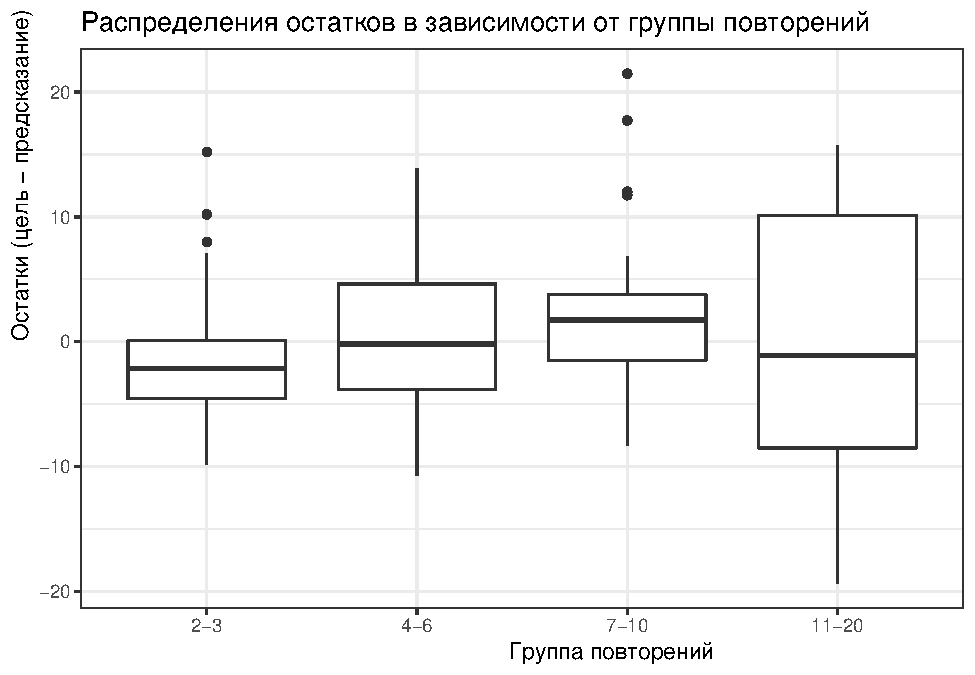
\includegraphics[width=0.9\linewidth]{Regression-model-for-estimating-RM_files/figure-latex/unnamed-chunk-32-1} \end{center}

\begin{center}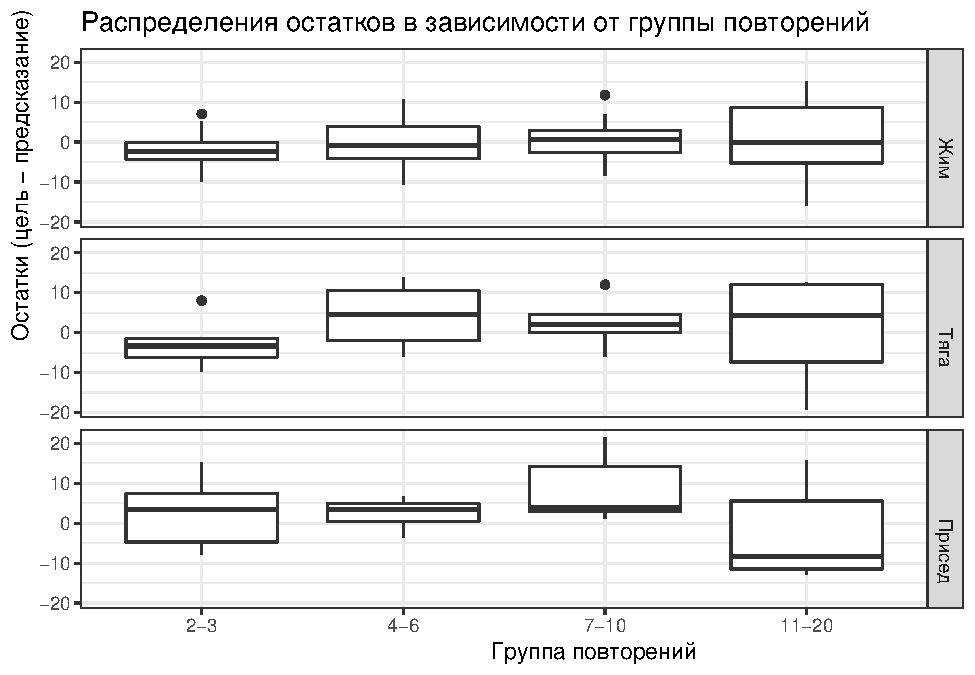
\includegraphics[width=0.9\linewidth]{Regression-model-for-estimating-RM_files/figure-latex/unnamed-chunk-32-2} \end{center}

\begin{center}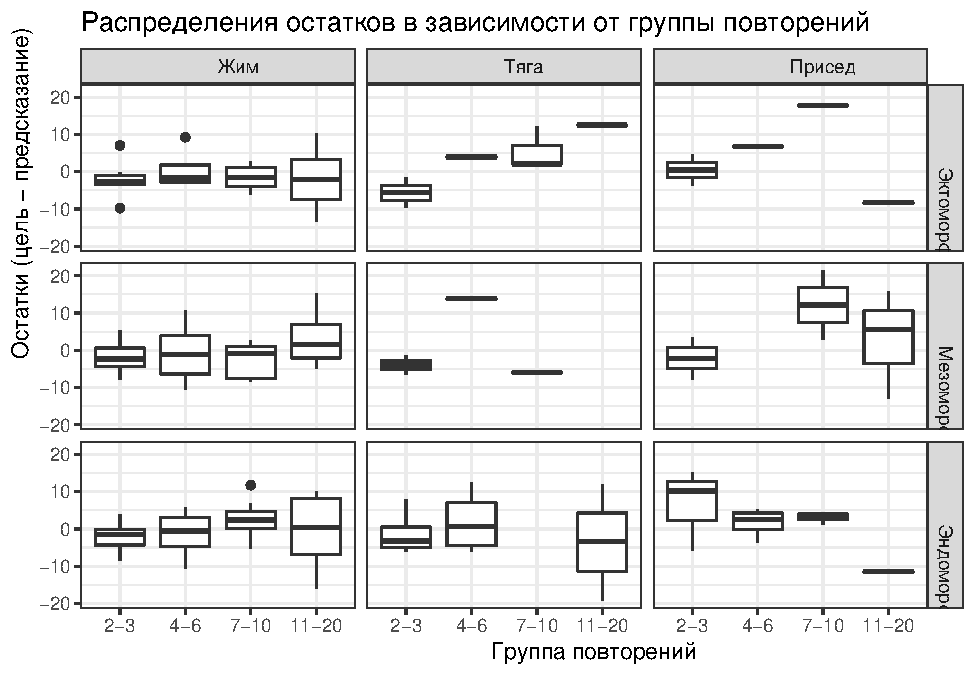
\includegraphics[width=0.9\linewidth]{Regression-model-for-estimating-RM_files/figure-latex/unnamed-chunk-32-3} \end{center}

\begin{verbatim}
## -----> ОБЩАЯ ИНФОРМАЦИЯ О МОДЕЛИ:
## 
## 
## Call:
## lm(formula = RM ~ MRM + MRM:Count - 1, data = data)
## 
## Residuals:
##      Min       1Q   Median       3Q      Max 
## -19.3323  -4.3200  -0.4872   3.9362  21.4700 
## 
## Coefficients:
##            Estimate Std. Error t value Pr(>|t|)    
## MRM       1.0470734  0.0067757  154.53   <2e-16 ***
## MRM:Count 0.0209793  0.0008774   23.91   <2e-16 ***
## ---
## Signif. codes:  0 '***' 0.001 '**' 0.01 '*' 0.05 '.' 0.1 ' ' 1
## 
## Residual standard error: 6.698 on 160 degrees of freedom
## Multiple R-squared:  0.9983, Adjusted R-squared:  0.9983 
## F-statistic: 4.664e+04 on 2 and 160 DF,  p-value: < 2.2e-16
## 
## 
## ASSESSMENT OF THE LINEAR MODEL ASSUMPTIONS
## USING THE GLOBAL TEST ON 4 DEGREES-OF-FREEDOM:
## Level of Significance =  0.05 
## 
## Call:
##  gvlma::gvlma(x = mdl) 
## 
##                      Value  p-value                   Decision
## Global Stat        15.1022 0.004494 Assumptions NOT satisfied!
## Skewness            3.1467 0.076078    Assumptions acceptable.
## Kurtosis            1.9628 0.161218    Assumptions acceptable.
## Link Function       0.2725 0.601627    Assumptions acceptable.
## Heteroscedasticity  9.7202 0.001823 Assumptions NOT satisfied!
##                         Value     p-value                   Decision
## Global Stat        15.1022329 0.004493809 Assumptions NOT satisfied!
## Skewness            3.1467476 0.076078463    Assumptions acceptable.
## Kurtosis            1.9627685 0.161217544    Assumptions acceptable.
## Link Function       0.2725495 0.601626657    Assumptions acceptable.
## Heteroscedasticity  9.7201673 0.001822569 Assumptions NOT satisfied!
## 
## -----> БАЗОВЫЕ ГРАФИКИ:
\end{verbatim}

\begin{center}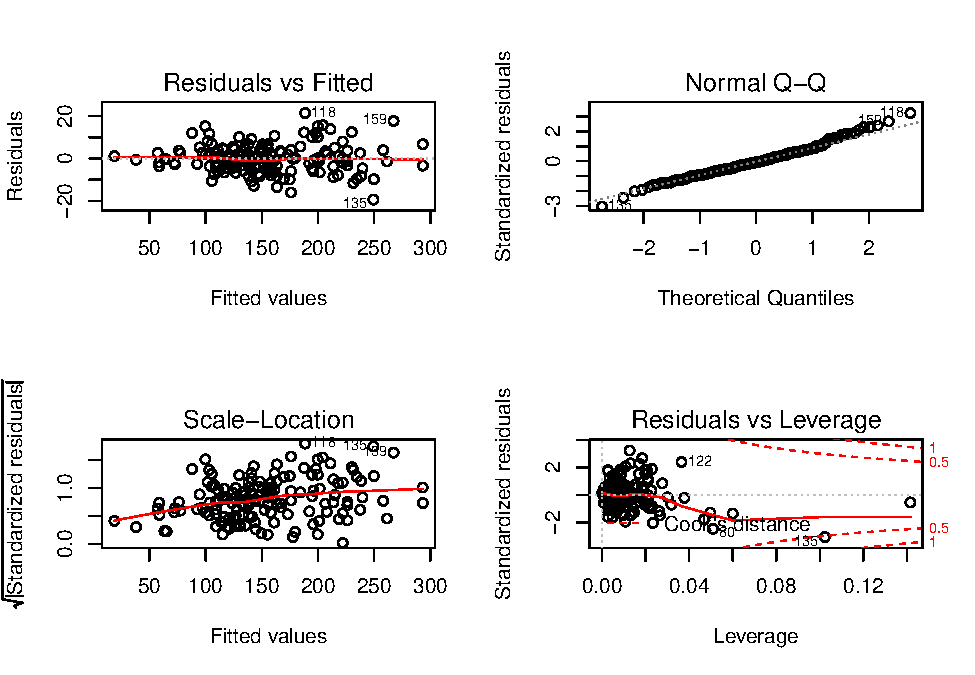
\includegraphics[width=0.9\linewidth]{Regression-model-for-estimating-RM_files/figure-latex/unnamed-chunk-32-4} \end{center}

\begin{verbatim}
## 
## -----> ТЕСТ НА НОРМАЛЬНОСТЬ РАСПРЕДЕЛЕНИЯ ОСТАТКОВ
## 
## 
##  Shapiro-Wilk normality test
## 
## data:  mdl$residuals
## W = 0.98782, p-value = 0.1726
\end{verbatim}

\begin{center}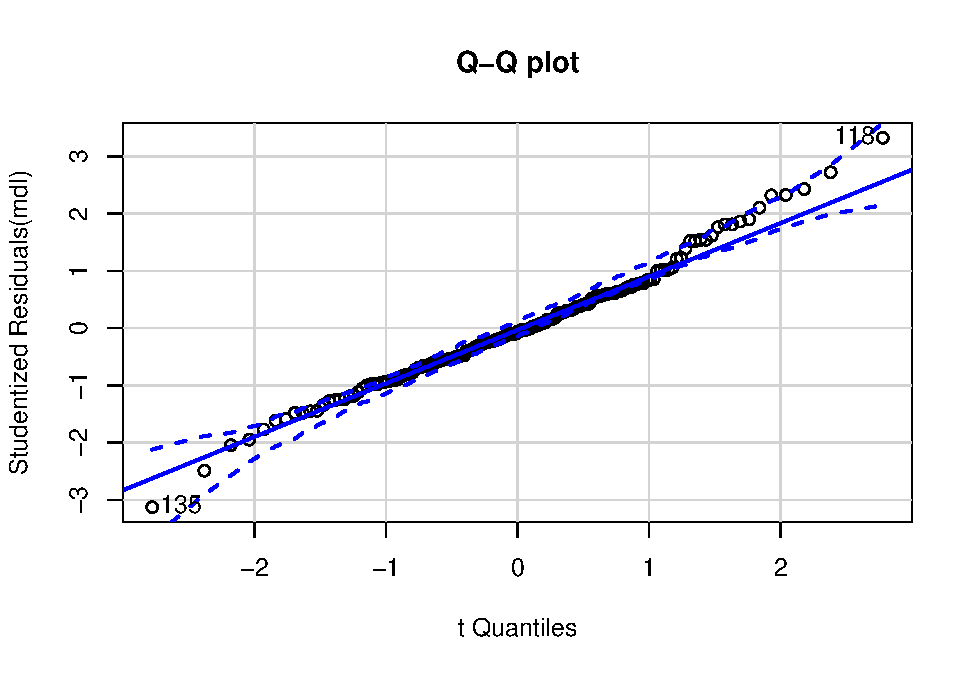
\includegraphics[width=0.9\linewidth]{Regression-model-for-estimating-RM_files/figure-latex/unnamed-chunk-32-5} \end{center}

\begin{verbatim}
## -----> ФАКТОР ИНФЛЯЦИИ ДИСПЕРСИЙ:
## 
##       MRM MRM:Count 
##  3.057194  3.057194 
## 
## -----> ТЕСТ НА АВТОКОРРЕЛЯЦИЮ:
## 
##  lag Autocorrelation D-W Statistic p-value
##    1      0.07681102      1.839824   0.254
##  Alternative hypothesis: rho != 0
## 
## -----> ТЕСТ НА ВЫБРОСЫ И ВЛИЯТЕЛЬНЫЕ НАБЛЮДЕНИЯ:
## 
## No Studentized residuals with Bonferroni p < 0.05
## Largest |rstudent|:
##     rstudent unadjusted p-value Bonferroni p
## 118 3.325731          0.0010952      0.17741
\end{verbatim}

\begin{center}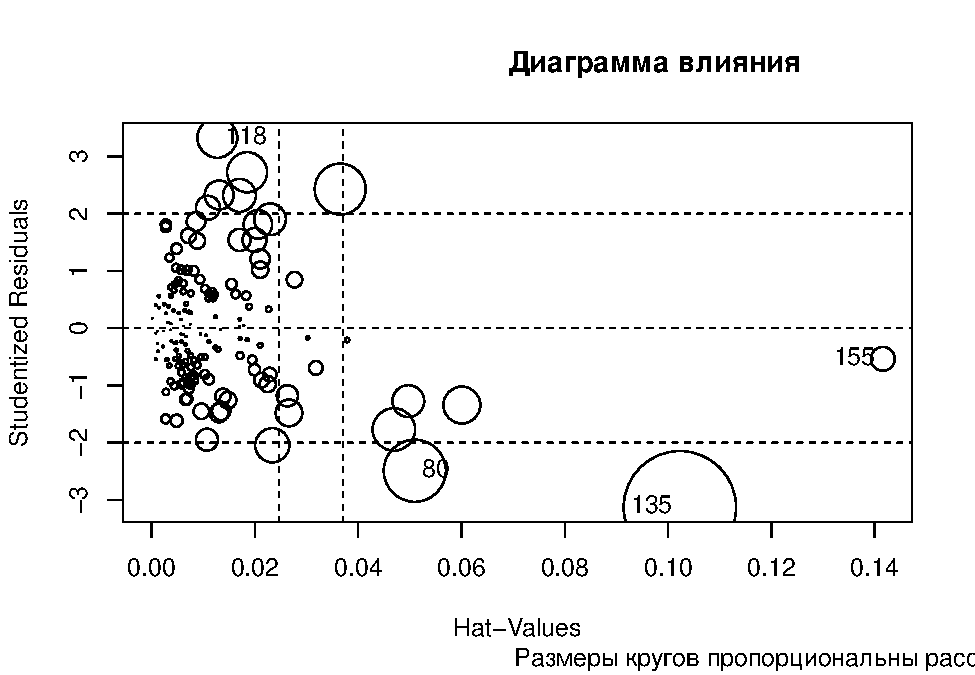
\includegraphics[width=0.9\linewidth]{Regression-model-for-estimating-RM_files/figure-latex/unnamed-chunk-32-6} \end{center}

\begin{verbatim}
## -----> ВЫБРОСЫ И ВЛИЯТЕЛЬНЫЕ НАБЛЮДЕНИЯ:
## 
## 
## |  RM| MRM| Count|Action |Sex     |Experience    | Age| Weight| Height|BodyType |IndexGroup |
## |---:|---:|-----:|:------|:-------|:-------------|---:|------:|------:|:--------|:----------|
## | 290| 200|    20|Тяга   |Мужчина |6-10 лет      |  28|    107|    185|Эндоморф |ожирение1  |
## | 230| 170|    20|Тяга   |Мужчина |6-10 лет      |  25|     82|    178|Эндоморф |избыток    |
## | 210| 150|    10|Присед |Мужчина |больше 10 лет |  42|    100|    183|Мезоморф |избыток    |
## | 160| 120|    20|Жим    |Мужчина |4-5 лет       |  22|    115|    195|Эндоморф |ожирение1  |
\end{verbatim}

Выше приведена вся необходимая информация о качестве модели (назовём эту
модель \(b_1\)). Из неё важнее всего следующее:

\begin{itemize}
\item
  На выборочных данных модель ошибается максимум на 21кг и 13\%;
\item
  В среднем модель ошибается на 3\%;
\item
  В 75\% случаев ошибка не превышала 5\%;
\item
  Наибольший разброс ошибок приходится на диапазон 11-20;
\item
  Модель статистически значима и удовлетворяет всем нужным требованиям,
  кроме гетероскедастичности;
\item
  Немало больших ошибок приходится на диапазон 11-20 повторений,
  содержащий меньше всего наблюдений.
\end{itemize}

\hypertarget{ux443ux442ux43eux447ux43dux435ux43dux438ux435-ux43aux43eux44dux444ux444ux438ux446ux438ux435ux43dux442ux43eux432-ux437ux430ux432ux438ux441ux438ux43cux43eux441ux442ux44c-ux43eux442-ux434ux438ux430ux43fux430ux437ux43eux43dux430}{%
\subsection{Уточнение коэффициентов: зависимость от
диапазона}\label{ux443ux442ux43eux447ux43dux435ux43dux438ux435-ux43aux43eux44dux444ux444ux438ux446ux438ux435ux43dux442ux43eux432-ux437ux430ux432ux438ux441ux438ux43cux43eux441ux442ux44c-ux43eux442-ux434ux438ux430ux43fux430ux437ux43eux43dux430}}

Теперь сделаем поправку для коэффициентов \(a,b\) в зависимости от
факторных переменных.

Путём подбора удалось найти две схожие модели (назовём их \(b_2\) и
\(b_3\)), немного отличающиеся оценками кросс-валидации на разных
диапазонах. \textbf{Поскольку на диапазоне повторений 11-20 по-прежнему
сохранялись сильные ошибки, было принято решение удалить этот диапазон}
(также это можно обосновать тем, что на этом диапазоне меньше данных и
сложнее отлавливать выбросы, да и физиологически он не так тесно связан
с силой, как другие, о чём уже было сказано).

Далее приведён анализ для модели \(RM=MRM \cdot(a+b \cdot Count)\), в
которой и \(a\) и \(b\) имеют поправку на диапазон повторений.

\begin{verbatim}
## Ошибки модели (выведены 15 элементов с наибольшими ошибками): 
## 
## 
## | Fact| Target|     ERROR| ErrorPercent|   MRM| Count|Action |Sex     | Weight|CountGroup |    Index|
## |----:|------:|---------:|------------:|-----:|-----:|:------|:-------|------:|:----------|--------:|
## |  192|    210| 18.248827|     8.689918| 150.0|    10|Присед |Мужчина |    100|7-10       | 29.86055|
## |  199|    215| 15.665296|     7.286184| 180.0|     3|Присед |Мужчина |     84|2-3        | 30.11940|
## |  271|    285| 14.260782|     5.003783| 220.0|     8|Присед |Мужчина |     90|7-10       | 30.07117|
## |  142|    130| 12.462268|     9.586360| 120.0|     6|Жим    |Мужчина |     98|4-6        | 27.72748|
## |  237|    225| 12.437114|     5.527606| 200.0|     6|Жим    |Мужчина |    102|4-6        | 30.12760|
## |  107|     95| 11.846701|    12.470212|  90.0|     6|Жим    |Мужчина |     74|4-6        | 23.62029|
## |  214|    225| 11.306598|     5.025155| 180.0|     6|Тяга   |Мужчина |     90|4-6        | 26.29657|
## |  199|    210| 10.665296|     5.078712| 180.0|     3|Присед |Мужчина |    125|2-3        | 36.13134|
## |  141|    130| 10.617527|     8.167328| 110.0|    10|Жим    |Мужчина |    100|7-10       | 28.29335|
## |  151|    140| 10.538438|     7.527456| 120.0|     9|Жим    |Мужчина |     77|7-10       | 28.62879|
## |   89|    100| 10.516119|    10.516119|  70.0|    10|Тяга   |Мужчина |     63|7-10       | 19.23018|
## |  105|    115| 10.396211|     9.040184|  85.0|     8|Жим    |Мужчина |     76|7-10       | 25.10239|
## |  162|    172| 10.219244|     5.941421| 140.0|     5|Жим    |Мужчина |     83|4-6        | 27.73230|
## |  190|    200| 10.050309|     5.025155| 160.0|     6|Тяга   |Мужчина |    120|4-6        | 34.68609|
## |  174|    165|  9.417866|     5.707798| 157.5|     3|Жим    |Мужчина |     87|2-3        | 26.85185|
## 
## ------------> Наибольшая ошибка в большую сторону: 12.46227 
## ------------> Наибольшая ошибка в меньшую сторону: 18.24883 
## Модель ошиблась более чем на 5 % в 28 случаях из 139 ( 20.14388 %)
## Модель ошиблась более чем на 5 кг в 44 случаях из 139 ( 31.65468 %)
## ----------------> Статистика по ошибкам в процентах:
##     Min.  1st Qu.   Median     Mean  3rd Qu.     Max. 
##  0.00977  0.91712  2.53843  2.98739  4.29788 12.47021 
## -------------------> Среднеквадратичная ошибка: 5.529521 
## Оценка кросс-валидации для всего набора данных 33.88957 
## Оценка кросс-валидации для не более чем 10 повторений 33.62558 
## Оценка кросс-валидации для не более чем 6 повторений 30.93245
\end{verbatim}

\begin{center}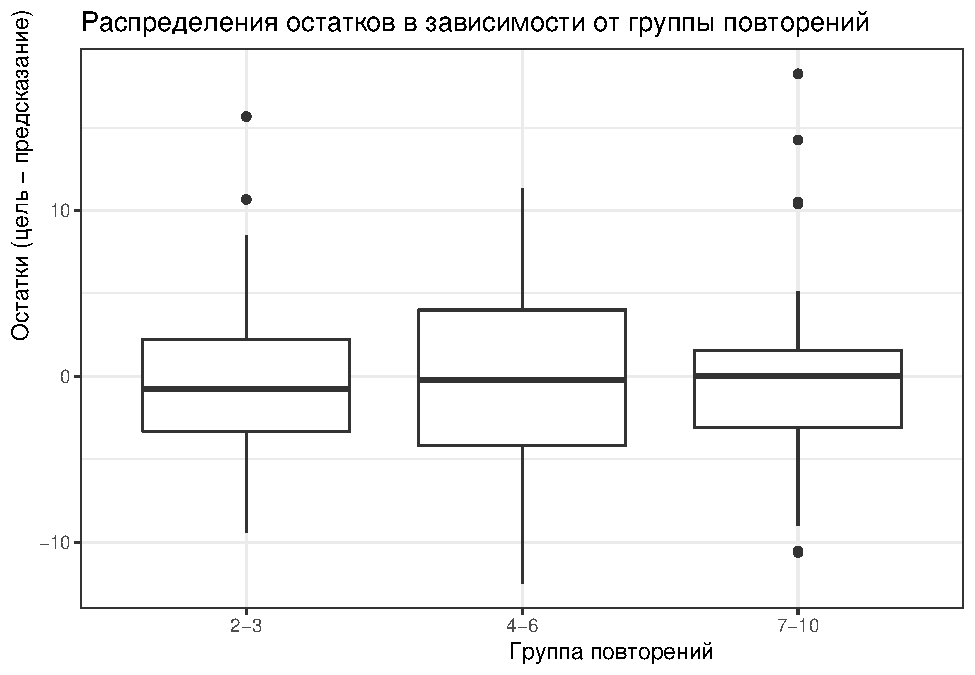
\includegraphics{Regression-model-for-estimating-RM_files/figure-latex/unnamed-chunk-33-1} \end{center}

\begin{center}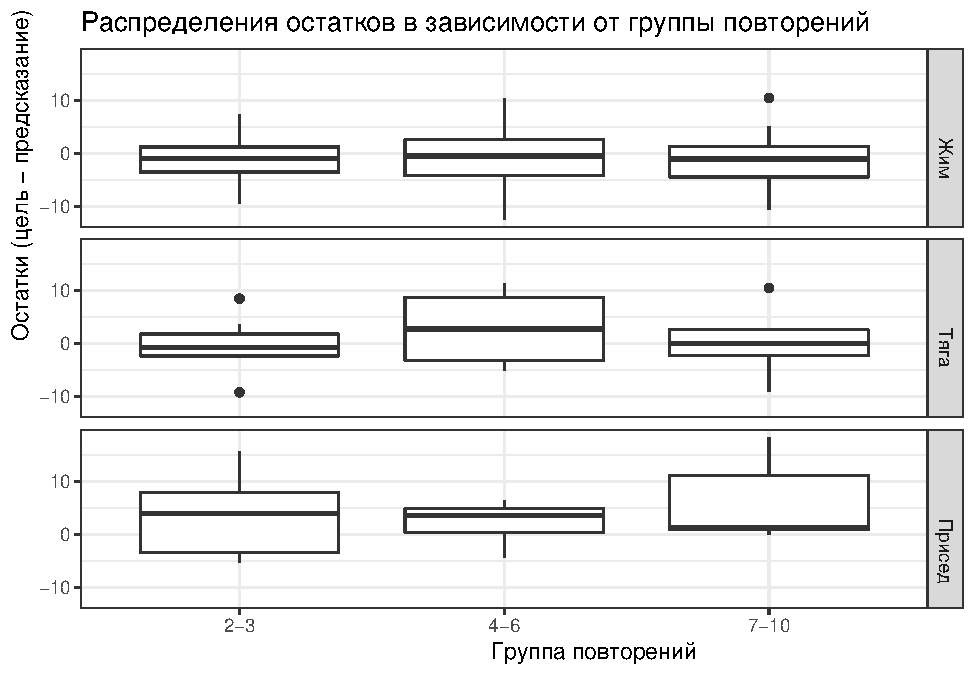
\includegraphics{Regression-model-for-estimating-RM_files/figure-latex/unnamed-chunk-33-2} \end{center}

\begin{center}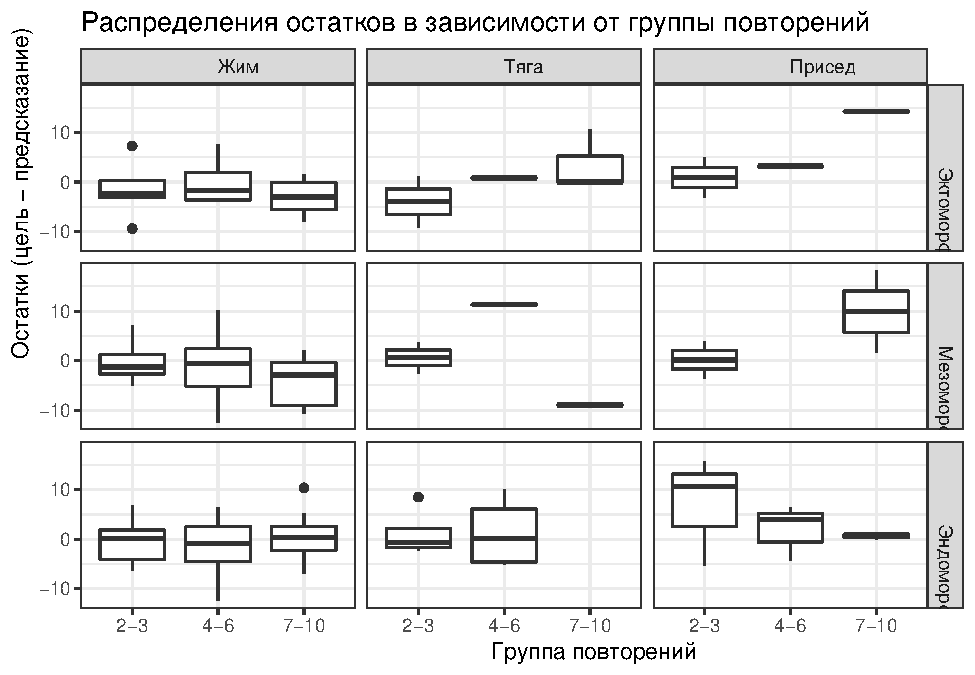
\includegraphics{Regression-model-for-estimating-RM_files/figure-latex/unnamed-chunk-33-3} \end{center}

\begin{verbatim}
## -----> ОБЩАЯ ИНФОРМАЦИЯ О МОДЕЛИ:
## 
## 
## Call:
## lm(formula = RM ~ MRM:Count:CountGroup + MRM:CountGroup - 1, 
##     data = data)
## 
## Residuals:
##      Min       1Q   Median       3Q      Max 
## -12.4623  -3.6210  -0.1014   2.5825  18.2488 
## 
## Coefficients:
##                          Estimate Std. Error t value Pr(>|t|)    
## MRM:CountGroup2-3        0.988699   0.029669  33.324  < 2e-16 ***
## MRM:CountGroup4-6        0.997533   0.035651  27.981  < 2e-16 ***
## MRM:CountGroup7-10       1.039799   0.055896  18.603  < 2e-16 ***
## MRM:Count:CountGroup2-3  0.039572   0.011331   3.492 0.000650 ***
## MRM:Count:CountGroup4-6  0.031609   0.007065   4.474 1.63e-05 ***
## MRM:Count:CountGroup7-10 0.023854   0.006434   3.708 0.000306 ***
## ---
## Signif. codes:  0 '***' 0.001 '**' 0.01 '*' 0.05 '.' 0.1 ' ' 1
## 
## Residual standard error: 5.653 on 133 degrees of freedom
## Multiple R-squared:  0.9987, Adjusted R-squared:  0.9987 
## F-statistic: 1.768e+04 on 6 and 133 DF,  p-value: < 2.2e-16
## 
## 
## ASSESSMENT OF THE LINEAR MODEL ASSUMPTIONS
## USING THE GLOBAL TEST ON 4 DEGREES-OF-FREEDOM:
## Level of Significance =  0.05 
## 
## Call:
##  gvlma::gvlma(x = mdl) 
## 
##                     Value p-value                   Decision
## Global Stat         8.359 0.07929    Assumptions acceptable.
## Skewness            2.795 0.09455    Assumptions acceptable.
## Kurtosis            2.394 0.12180    Assumptions acceptable.
## Link Function      -2.689 1.00000    Assumptions acceptable.
## Heteroscedasticity  5.858 0.01550 Assumptions NOT satisfied!
##                        Value    p-value                   Decision
## Global Stat         8.358530 0.07929330    Assumptions acceptable.
## Skewness            2.795168 0.09454886    Assumptions acceptable.
## Kurtosis            2.394055 0.12179736    Assumptions acceptable.
## Link Function      -2.689003 1.00000000    Assumptions acceptable.
## Heteroscedasticity  5.858310 0.01550367 Assumptions NOT satisfied!
## 
## -----> БАЗОВЫЕ ГРАФИКИ:
\end{verbatim}

\begin{center}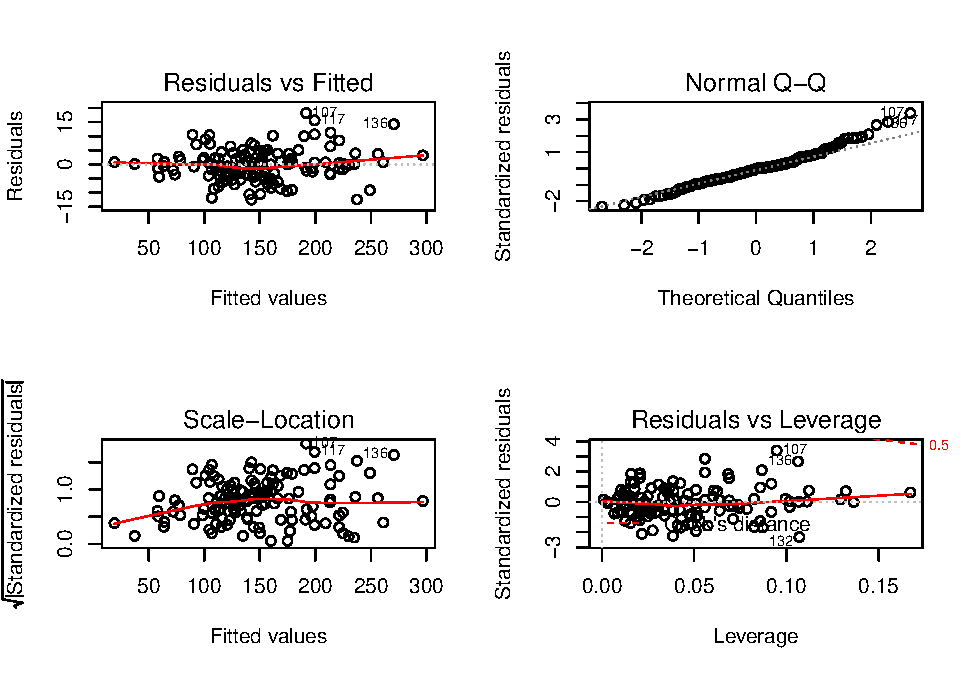
\includegraphics{Regression-model-for-estimating-RM_files/figure-latex/unnamed-chunk-33-4} \end{center}

\begin{verbatim}
## 
## -----> ТЕСТ НА НОРМАЛЬНОСТЬ РАСПРЕДЕЛЕНИЯ ОСТАТКОВ
## 
## 
##  Shapiro-Wilk normality test
## 
## data:  mdl$residuals
## W = 0.98086, p-value = 0.0484
\end{verbatim}

\begin{center}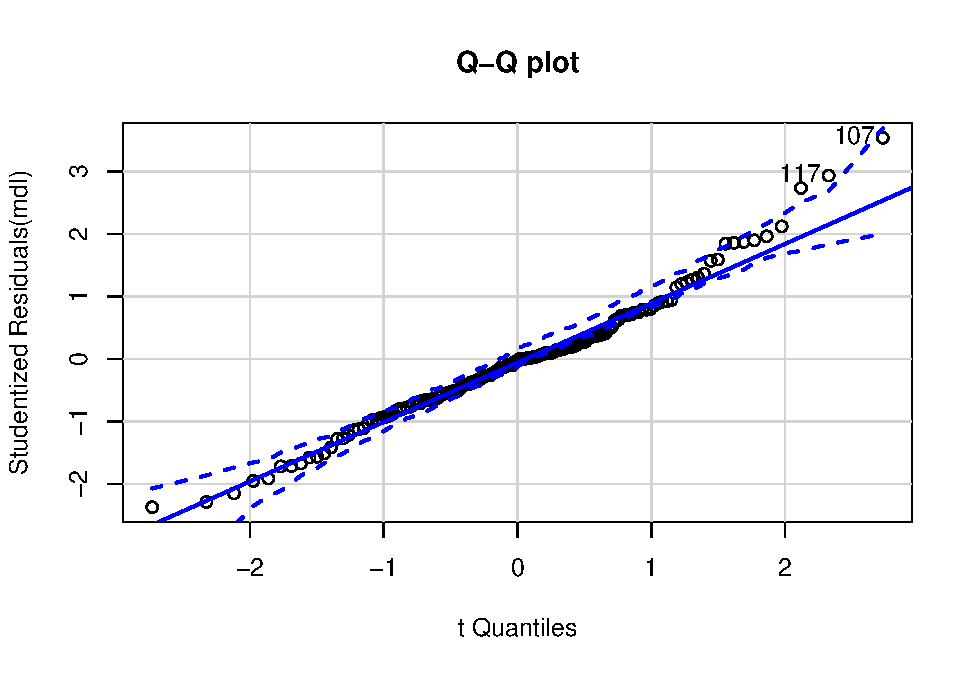
\includegraphics{Regression-model-for-estimating-RM_files/figure-latex/unnamed-chunk-33-5} \end{center}

\begin{verbatim}
## -----> ФАКТОР ИНФЛЯЦИИ ДИСПЕРСИЙ:
## 
##                          GVIF Df GVIF^(1/(2*Df))
## MRM:CountGroup       60763.96  3        6.270098
## MRM:Count:CountGroup 60763.96  3        6.270098
## 
## -----> ТЕСТ НА АВТОКОРРЕЛЯЦИЮ:
## 
##  lag Autocorrelation D-W Statistic p-value
##    1      -0.0176863      2.032798    0.93
##  Alternative hypothesis: rho != 0
## 
## -----> ТЕСТ НА ВЫБРОСЫ И ВЛИЯТЕЛЬНЫЕ НАБЛЮДЕНИЯ:
## 
## No Studentized residuals with Bonferroni p < 0.05
## Largest |rstudent|:
##     rstudent unadjusted p-value Bonferroni p
## 107  3.53666         0.00055969     0.077797
\end{verbatim}

\begin{center}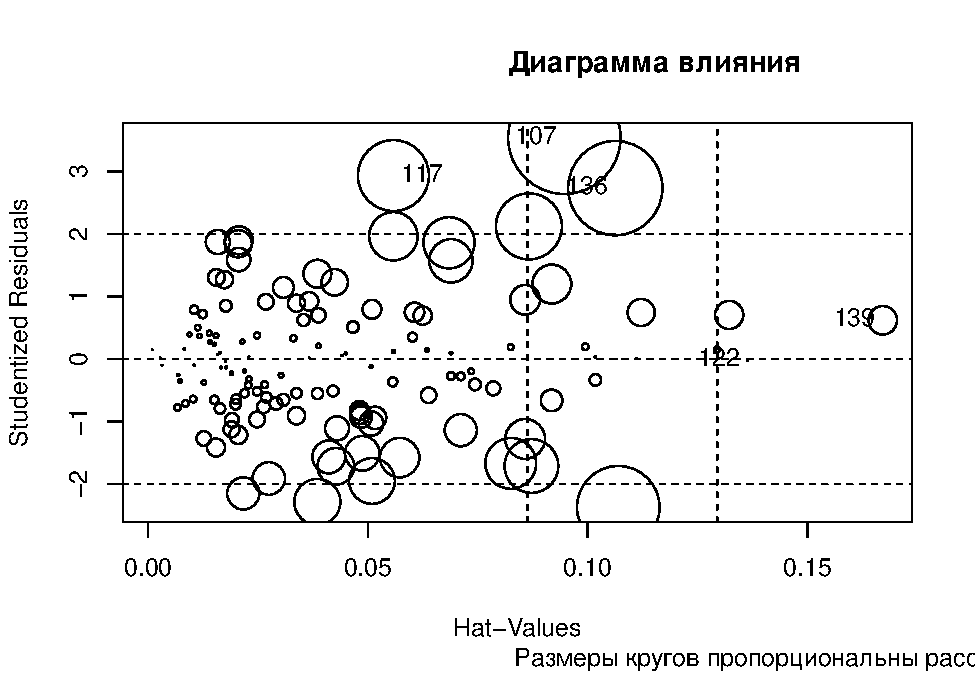
\includegraphics{Regression-model-for-estimating-RM_files/figure-latex/unnamed-chunk-33-6} \end{center}

\begin{verbatim}
## -----> ВЫБРОСЫ И ВЛИЯТЕЛЬНЫЕ НАБЛЮДЕНИЯ:
## 
## 
## |  RM| MRM| Count|Action |Sex     |Experience    | Age| Weight| Height|BodyType |IndexGroup |
## |---:|---:|-----:|:------|:-------|:-------------|---:|------:|------:|:--------|:----------|
## | 300| 250|     6|Присед |Мужчина |больше 10 лет |  28|    117|    193|Эктоморф |ожирение1  |
## | 285| 220|     8|Присед |Мужчина |больше 10 лет |  35|     90|    173|Эктоморф |ожирение1  |
## | 230| 180|    10|Присед |Мужчина |4-5 лет       |  24|    104|    182|Эндоморф |ожирение1  |
## | 215| 180|     3|Присед |Мужчина |4-5 лет       |  20|     84|    167|Эндоморф |ожирение1  |
## | 210| 150|    10|Присед |Мужчина |больше 10 лет |  42|    100|    183|Мезоморф |избыток    |
\end{verbatim}

Аналогичные выводы:

\begin{itemize}
\item
  На выборочных данных модель ошибается максимум на 18кг и 13\%;
\item
  В среднем модель ошибается на 3\%;
\item
  В 80\% случаев ошибка не превышала 5\%;
\item
  Наибольший разброс ошибок приходится на диапазон 4-6;
\item
  Модель статистически значима и удовлетворяет всем нужным требованиям,
  кроме гетероскедастичности.
\end{itemize}

\hypertarget{ux442ux440ux435ux442ux44cux435-ux43fux43eux43aux43eux43bux435ux43dux438ux435-ux43cux43eux434ux435ux43bux435ux439}{%
\subsection{Третье поколение
моделей}\label{ux442ux440ux435ux442ux44cux435-ux43fux43eux43aux43eux43bux435ux43dux438ux435-ux43cux43eux434ux435ux43bux435ux439}}

Путём пошагового отбора переменных были найдены ещё две равнозначные
модели (\(b_4\) и \(b_5\)), которые, несмотря на б\textbf{о}льшую
сложность в сравнении с предыдущими, имеют лучшие оценки при
кросс-валидации.

Статистика для модели \(b_5\):

\begin{verbatim}
## Ошибки модели (выведены 15 элементов с наибольшими ошибками): 
## 
## 
## | Fact| Target|     ERROR| ErrorPercent| MRM| Count|Action |Sex     | Weight|CountGroup |    Index|
## |----:|------:|---------:|------------:|---:|-----:|:------|:-------|------:|:----------|--------:|
## |  196|  210.0| 13.900432|     6.619254| 150|    10|Присед |Мужчина |    100|7-10       | 29.86055|
## |  142|  130.0| 12.097350|     9.305654| 120|     6|Жим    |Мужчина |     98|4-6        | 27.72748|
## |  107|   95.0| 11.628844|    12.240888|  90|     6|Жим    |Мужчина |     74|4-6        | 23.62029|
## |  161|  172.0| 11.494330|     6.682750| 140|     5|Жим    |Мужчина |     83|4-6        | 27.73230|
## |  104|  115.0| 11.002650|     9.567522|  85|     8|Жим    |Мужчина |     76|7-10       | 25.10239|
## |  205|  215.0| 10.097807|     4.696655| 180|     3|Присед |Мужчина |     84|2-3        | 30.11940|
## |  100|  110.0|  9.891911|     8.992646|  90|     4|Жим    |Мужчина |     60|4-6        | 21.25850|
## |   90|  100.0|  9.795772|     9.795772|  70|    10|Тяга   |Мужчина |     63|7-10       | 19.23018|
## |  137|  127.5|  9.766699|     7.660156| 120|     3|Присед |Женщина |     72|2-3        | 26.76978|
## |  235|  225.0|  9.598310|     4.265916| 200|     6|Жим    |Мужчина |    102|4-6        | 30.12760|
## |  180|  170.0|  9.526585|     5.603874| 140|    10|Тяга   |Мужчина |     77|7-10       | 24.57787|
## |  216|  225.0|  9.425832|     4.189259| 180|     6|Тяга   |Мужчина |     90|4-6        | 26.29657|
## |  276|  285.0|  9.331980|     3.274379| 220|     8|Присед |Мужчина |     90|7-10       | 30.07117|
## |  149|  140.0|  8.921184|     6.372274| 120|     9|Жим    |Мужчина |     77|7-10       | 28.62879|
## |  139|  130.0|  8.573017|     6.594628| 110|    10|Жим    |Мужчина |    100|7-10       | 28.29335|
## 
## ------------> Наибольшая ошибка в большую сторону: 12.09735 
## ------------> Наибольшая ошибка в меньшую сторону: 13.90043 
## Модель ошиблась более чем на 5 % в 21 случаях из 139 ( 15.10791 %)
## Модель ошиблась более чем на 5 кг в 44 случаях из 139 ( 31.65468 %)
## ----------------> Статистика по ошибкам в процентах:
##     Min.  1st Qu.   Median     Mean  3rd Qu.     Max. 
##  0.01759  0.94961  2.08660  2.83833  3.94832 12.31595 
## -------------------> Среднеквадратичная ошибка: 5.026615 
## Оценка кросс-валидации для всего набора данных 29.34396 
## Оценка кросс-валидации для не более чем 10 повторений 30.23471 
## Оценка кросс-валидации для не более чем 6 повторений 28.26897
\end{verbatim}

\begin{center}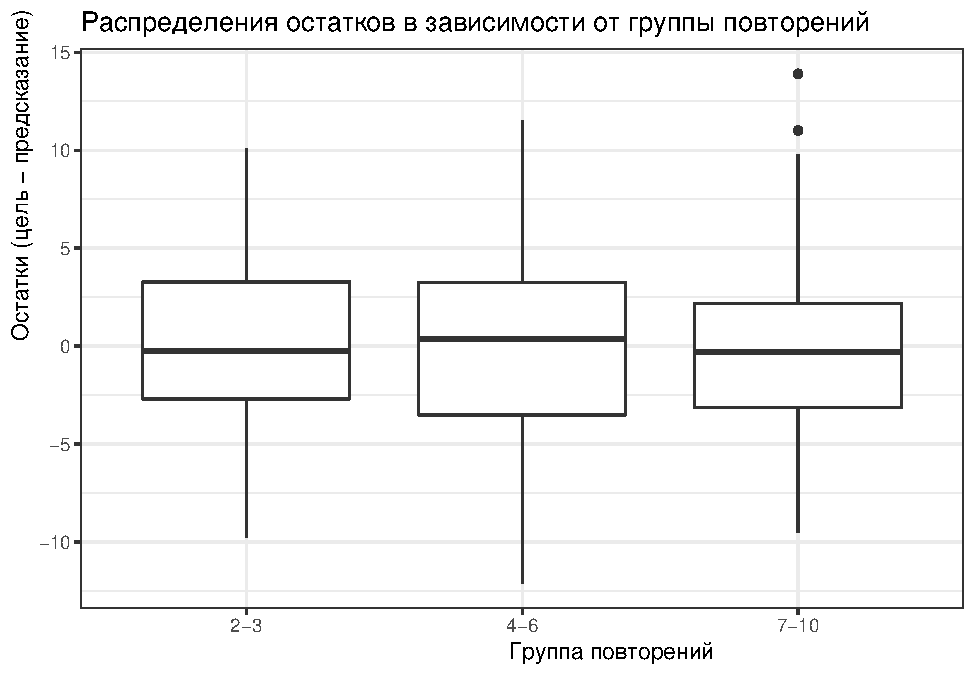
\includegraphics{Regression-model-for-estimating-RM_files/figure-latex/unnamed-chunk-34-1} \end{center}

\begin{center}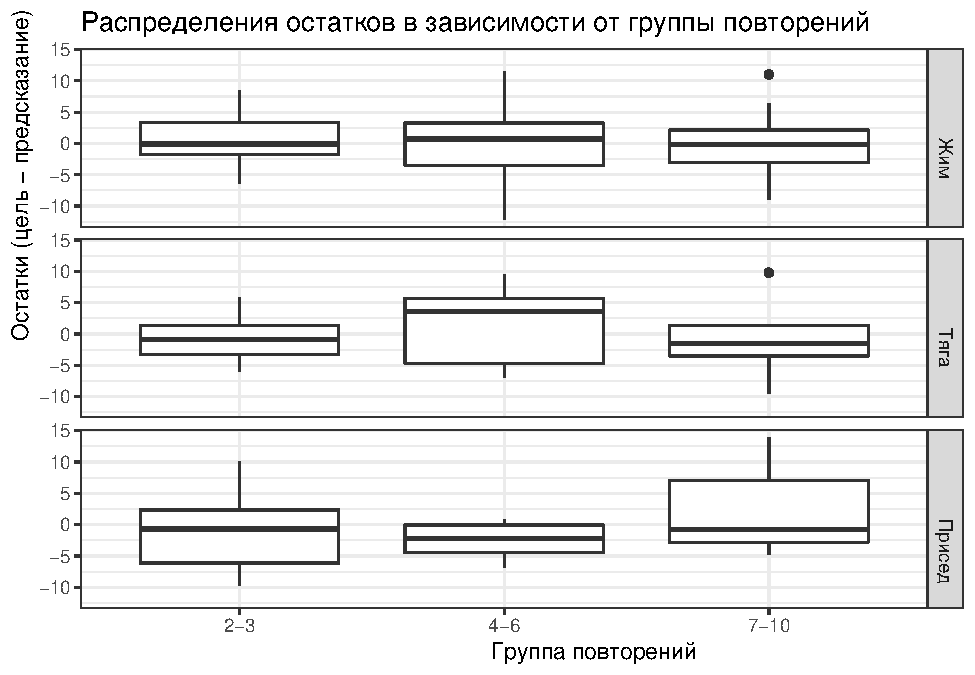
\includegraphics{Regression-model-for-estimating-RM_files/figure-latex/unnamed-chunk-34-2} \end{center}

\begin{center}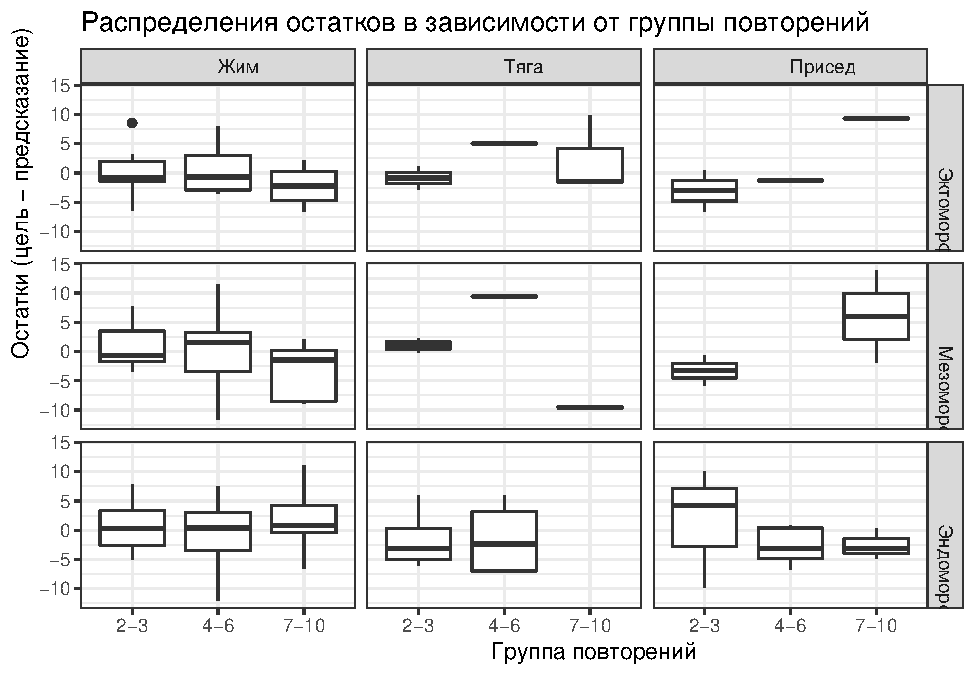
\includegraphics{Regression-model-for-estimating-RM_files/figure-latex/unnamed-chunk-34-3} \end{center}

\begin{verbatim}
## -----> ОБЩАЯ ИНФОРМАЦИЯ О МОДЕЛИ:
## 
## 
## Call:
## lm(formula = RM ~ I((MRM/Index)^6) + MRM:CountGroup + MRM:Action + 
##     MRM:CountGroup:Count - 1, data = data)
## 
## Residuals:
##      Min       1Q   Median       3Q      Max 
## -12.0974  -3.2898  -0.1568   3.0781  13.9004 
## 
## Coefficients:
##                            Estimate Std. Error t value Pr(>|t|)    
## I((MRM/Index)^6)         -2.989e-05  1.125e-05  -2.657  0.00887 ** 
## MRM:CountGroup2-3         9.963e-01  2.848e-02  34.984  < 2e-16 ***
## MRM:CountGroup4-6         9.711e-01  3.401e-02  28.558  < 2e-16 ***
## MRM:CountGroup7-10        1.077e+00  5.195e-02  20.738  < 2e-16 ***
## MRM:ActionТяга            2.893e-02  1.014e-02   2.854  0.00502 ** 
## MRM:ActionПрисед          4.984e-02  9.648e-03   5.166 8.78e-07 ***
## MRM:CountGroup2-3:Count   3.325e-02  1.067e-02   3.116  0.00226 ** 
## MRM:CountGroup4-6:Count   3.578e-02  6.842e-03   5.229 6.62e-07 ***
## MRM:CountGroup7-10:Count  1.833e-02  6.011e-03   3.050  0.00278 ** 
## ---
## Signif. codes:  0 '***' 0.001 '**' 0.01 '*' 0.05 '.' 0.1 ' ' 1
## 
## Residual standard error: 5.198 on 130 degrees of freedom
## Multiple R-squared:  0.999,  Adjusted R-squared:  0.9989 
## F-statistic: 1.395e+04 on 9 and 130 DF,  p-value: < 2.2e-16
## 
## 
## ASSESSMENT OF THE LINEAR MODEL ASSUMPTIONS
## USING THE GLOBAL TEST ON 4 DEGREES-OF-FREEDOM:
## Level of Significance =  0.05 
## 
## Call:
##  gvlma::gvlma(x = mdl) 
## 
##                      Value p-value                Decision
## Global Stat        2.19263  0.7004 Assumptions acceptable.
## Skewness           0.36972  0.5432 Assumptions acceptable.
## Kurtosis           0.02639  0.8710 Assumptions acceptable.
## Link Function      1.38357  0.2395 Assumptions acceptable.
## Heteroscedasticity 0.41295  0.5205 Assumptions acceptable.
##                         Value   p-value                Decision
## Global Stat        2.19262765 0.7003792 Assumptions acceptable.
## Skewness           0.36971780 0.5431581 Assumptions acceptable.
## Kurtosis           0.02639011 0.8709512 Assumptions acceptable.
## Link Function      1.38356953 0.2394941 Assumptions acceptable.
## Heteroscedasticity 0.41295021 0.5204759 Assumptions acceptable.
## 
## -----> БАЗОВЫЕ ГРАФИКИ:
\end{verbatim}

\begin{center}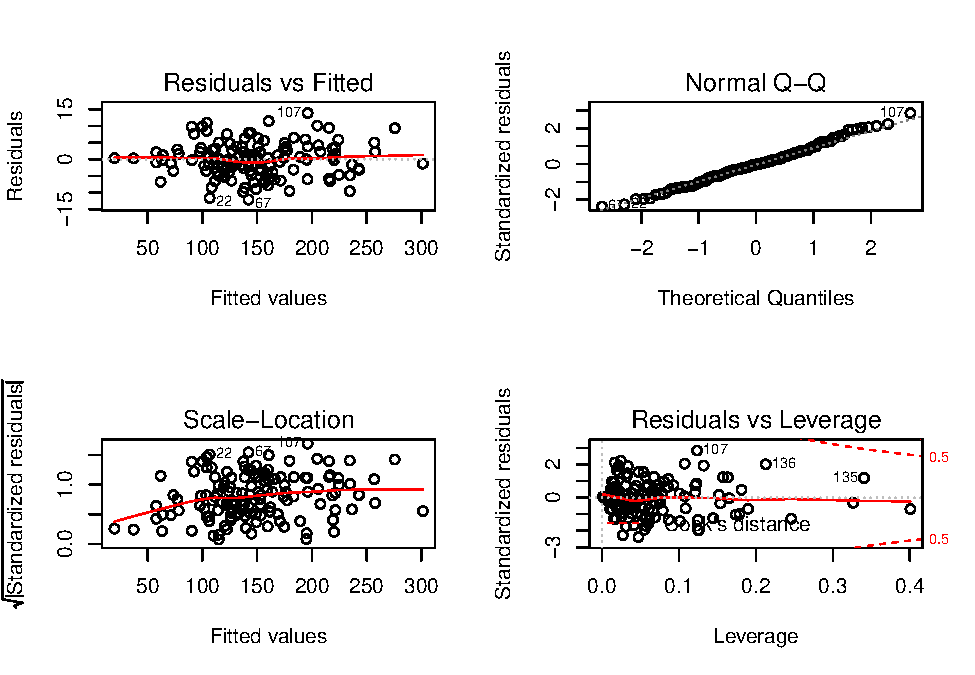
\includegraphics{Regression-model-for-estimating-RM_files/figure-latex/unnamed-chunk-34-4} \end{center}

\begin{verbatim}
## 
## -----> ТЕСТ НА НОРМАЛЬНОСТЬ РАСПРЕДЕЛЕНИЯ ОСТАТКОВ
## 
## 
##  Shapiro-Wilk normality test
## 
## data:  mdl$residuals
## W = 0.99366, p-value = 0.7982
\end{verbatim}

\begin{center}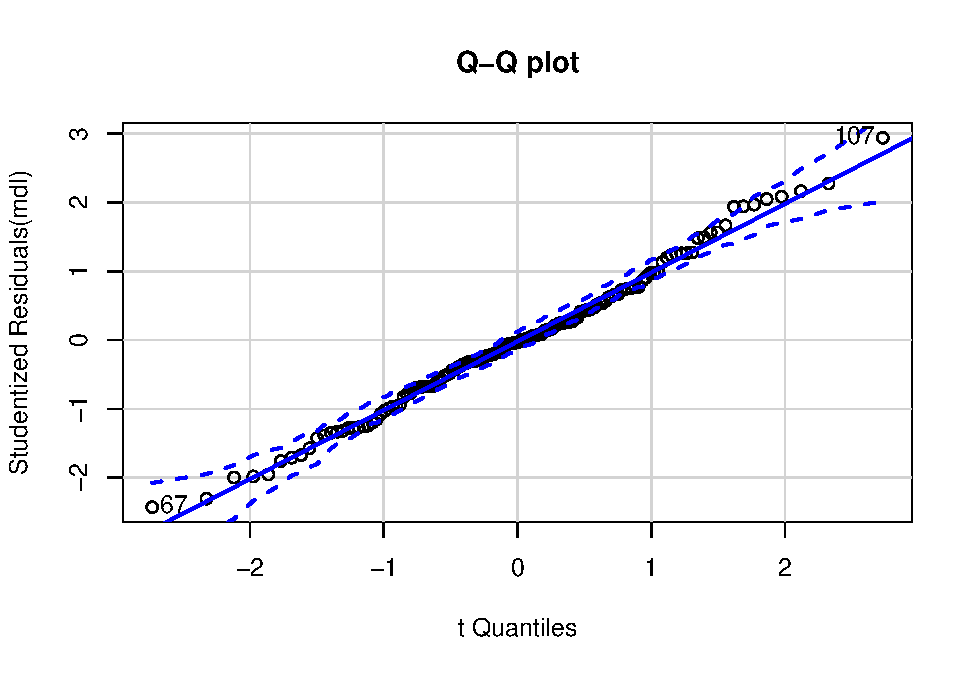
\includegraphics{Regression-model-for-estimating-RM_files/figure-latex/unnamed-chunk-34-5} \end{center}

\begin{verbatim}
## -----> ФАКТОР ИНФЛЯЦИИ ДИСПЕРСИЙ:
## 
##                              GVIF Df GVIF^(1/(2*Df))
## I((MRM/Index)^6)         2.561915  1        1.600598
## MRM:CountGroup       72443.114733  3        6.456535
## MRM:Action               2.898866  2        1.304839
## MRM:CountGroup:Count 72727.913065  3        6.460759
## 
## -----> ТЕСТ НА АВТОКОРРЕЛЯЦИЮ:
## 
##  lag Autocorrelation D-W Statistic p-value
##    1      0.05025135      1.898978   0.448
##  Alternative hypothesis: rho != 0
## 
## -----> ТЕСТ НА ВЫБРОСЫ И ВЛИЯТЕЛЬНЫЕ НАБЛЮДЕНИЯ:
## 
## No Studentized residuals with Bonferroni p < 0.05
## Largest |rstudent|:
##     rstudent unadjusted p-value Bonferroni p
## 107 2.939544           0.003896      0.54155
\end{verbatim}

\begin{center}\includegraphics{Regression-model-for-estimating-RM_files/figure-latex/unnamed-chunk-34-6} \end{center}

\begin{verbatim}
## -----> ВЫБРОСЫ И ВЛИЯТЕЛЬНЫЕ НАБЛЮДЕНИЯ:
## 
## 
## |  RM| MRM| Count|Action |Sex     |Experience    | Age| Weight| Height|BodyType |IndexGroup |
## |---:|---:|-----:|:------|:-------|:-------------|---:|------:|------:|:--------|:----------|
## | 285| 220|     8|Присед |Мужчина |больше 10 лет |  35|     90|    173|Эктоморф |ожирение1  |
## | 262| 220|     6|Тяга   |Мужчина |больше 10 лет |  33|     89|    184|Эктоморф |избыток    |
## | 240| 225|     3|Тяга   |Мужчина |больше 10 лет |  36|     87|    180|Эктоморф |избыток    |
## | 210| 150|    10|Присед |Мужчина |больше 10 лет |  42|    100|    183|Мезоморф |избыток    |
## | 130| 120|     6|Жим    |Мужчина |2-3 года      |  21|     98|    188|Эндоморф |избыток    |
\end{verbatim}

Аналогичные выводы:

\begin{itemize}
\item
  На выборочных данных модель ошибается максимум на 13кг и 12\%;
\item
  В среднем модель ошибается на менее 3\%;
\item
  В 85\% случаев ошибка не превышала 5\%;
\item
  В целом, на каждом диапазоне имеется почти одинаковый разброс;
\item
  Модель статистически значима и удовлетворяет всем нужным требованиям.
\end{itemize}

\begin{center}\rule{0.5\linewidth}{0.5pt}\end{center}

\hypertarget{ux441ux440ux430ux432ux43dux435ux43dux438ux435-ux43bux438ux43dux435ux439ux43dux44bux445-ux43cux43eux434ux435ux43bux435ux439-ux438-ux43fux43eux434ux432ux435ux434ux435ux43dux438ux435-ux438ux442ux43eux433ux43eux432}{%
\subsection{Сравнение линейных моделей и подведение
итогов}\label{ux441ux440ux430ux432ux43dux435ux43dux438ux435-ux43bux438ux43dux435ux439ux43dux44bux445-ux43cux43eux434ux435ux43bux435ux439-ux438-ux43fux43eux434ux432ux435ux434ux435ux43dux438ux435-ux438ux442ux43eux433ux43eux432}}

\begin{Shaded}
\begin{Highlighting}[]
\NormalTok{kn =}\StringTok{ }\KeywordTok{c}\NormalTok{(}\DecValTok{5}\NormalTok{, }\DecValTok{6}\NormalTok{, }\DecValTok{7}\NormalTok{, }\DecValTok{8}\NormalTok{, }\DecValTok{9}\NormalTok{, }\DecValTok{10}\NormalTok{, }\DecValTok{11}\NormalTok{, }\DecValTok{12}\NormalTok{)}

\NormalTok{ct =}\StringTok{ }\KeywordTok{c}\NormalTok{(}\DecValTok{8}\NormalTok{, }\DecValTok{11}\NormalTok{)}

\NormalTok{gr =}\StringTok{ }\KeywordTok{rep}\NormalTok{(}\KeywordTok{c}\NormalTok{(}\StringTok{"2-10"}\NormalTok{, }\StringTok{"2-7"}\NormalTok{), }\KeywordTok{length}\NormalTok{(kn)) }\OperatorTok\StringTok{ }\KeywordTok{sort}\NormalTok{(}\DataTypeTok{decreasing =}\NormalTok{ T)}

\NormalTok{m =}\StringTok{ }\KeywordTok{matrix}\NormalTok{(}\DataTypeTok{nrow =} \KeywordTok{length}\NormalTok{(kn) }\OperatorTok{*}\StringTok{ }\KeywordTok{length}\NormalTok{(ct), }\DataTypeTok{ncol =} \DecValTok{5}\NormalTok{)}

\NormalTok{lst =}\StringTok{ }\KeywordTok{list}\NormalTok{(b1, b2, b3, b4, b5)}


\ControlFlowTok{for}\NormalTok{ (i }\ControlFlowTok{in} \DecValTok{1}\OperatorTok{:}\DecValTok{5}\NormalTok{) \{}
    
\NormalTok{    model =}\StringTok{ }\NormalTok{lst[[i]]}
    
    \ControlFlowTok{for}\NormalTok{ (j }\ControlFlowTok{in} \DecValTok{1}\OperatorTok{:}\KeywordTok{length}\NormalTok{(ct)) \{}
\NormalTok{        dt =}\StringTok{ }\NormalTok{data }\OperatorTok\StringTok{ }\KeywordTok{filter}\NormalTok{(Count }\OperatorTok{<}\StringTok{ }\NormalTok{ct[j])}
\NormalTok{        gl =}\StringTok{ }\KeywordTok{glm}\NormalTok{(}\DataTypeTok{formula =}\NormalTok{ model}\OperatorTok{$}\NormalTok{call}\OperatorTok{$}\NormalTok{formula, }\DataTypeTok{data =}\NormalTok{ dt)}
        
\NormalTok{        getval =}\StringTok{ }\ControlFlowTok{function}\NormalTok{(k) \{}
\NormalTok{            boot}\OperatorTok{::}\KeywordTok{cv.glm}\NormalTok{(dt, gl, }\DataTypeTok{K =}\NormalTok{ k)}\OperatorTok{$}\NormalTok{delta[}\DecValTok{1}\NormalTok{] }\OperatorTok\StringTok{ }\KeywordTok{return}\NormalTok{()}
\NormalTok{        \}}
        
\NormalTok{        getval.mean =}\StringTok{ }\ControlFlowTok{function}\NormalTok{(k, count) \{}
            \KeywordTok{map_dbl}\NormalTok{(}\DecValTok{1}\OperatorTok{:}\NormalTok{count, }\ControlFlowTok{function}\NormalTok{(x) }\KeywordTok{getval}\NormalTok{(k)) }\OperatorTok\StringTok{ }\KeywordTok{mean}\NormalTok{() }\OperatorTok\StringTok{ }\KeywordTok{return}\NormalTok{()}
\NormalTok{        \}}
        
\NormalTok{        beg =}\StringTok{ }\NormalTok{(j }\OperatorTok{-}\StringTok{ }\DecValTok{1}\NormalTok{) }\OperatorTok{*}\StringTok{ }\KeywordTok{length}\NormalTok{(kn)}
        
        \ControlFlowTok{for}\NormalTok{ (s }\ControlFlowTok{in} \DecValTok{1}\OperatorTok{:}\KeywordTok{length}\NormalTok{(kn)) \{}
\NormalTok{            m[beg }\OperatorTok{+}\StringTok{ }\NormalTok{s, i] =}\StringTok{ }\KeywordTok{getval.mean}\NormalTok{(kn[s], }\DecValTok{30}\NormalTok{)}
\NormalTok{        \}}
        \CommentTok{# print(m)}
\NormalTok{    \}}
    
\NormalTok{\}}

\KeywordTok{colnames}\NormalTok{(m) =}\StringTok{ }\KeywordTok{paste0}\NormalTok{(}\StringTok{"b"}\NormalTok{, }\DecValTok{1}\OperatorTok{:}\DecValTok{5}\NormalTok{)}
\NormalTok{kp =}\StringTok{ }\KeywordTok{rep}\NormalTok{(kn, }\KeywordTok{length}\NormalTok{(ct))}

\NormalTok{vals =}\StringTok{ }\KeywordTok{data.frame}\NormalTok{(}\DataTypeTok{kp =} \KeywordTok{rep}\NormalTok{(kp, }\DecValTok{5}\NormalTok{), }\DataTypeTok{b =} \KeywordTok{as.numeric}\NormalTok{(m), }\DataTypeTok{gr =} \KeywordTok{factor}\NormalTok{(}\KeywordTok{rep}\NormalTok{(gr, }\DecValTok{5}\NormalTok{)), }\DataTypeTok{n =} \KeywordTok{factor}\NormalTok{(}\KeywordTok{rep}\NormalTok{(}\KeywordTok{colnames}\NormalTok{(m), }
    \KeywordTok{length}\NormalTok{(kn) }\OperatorTok{*}\StringTok{ }\KeywordTok{length}\NormalTok{(ct)) }\OperatorTok\StringTok{ }\KeywordTok{sort}\NormalTok{())) }\OperatorTok\StringTok{ }\KeywordTok{tbl_df}\NormalTok{()}
\end{Highlighting}
\end{Shaded}

В результате перекрёстной проверки для всех моделей при числе блоков 5,
6, 7, 8, 9, 10, 11, 12 было обнаружено, что модель \(b_5\) значительно
превосходит остальные модели, причём это верно, если делать проверку как
на всём диапазоне повторений (2-10), так и на более близком к силовому
диапазоне 2-7:

\begin{center}\includegraphics[width=0.95\linewidth]{Regression-model-for-estimating-RM_files/figure-latex/unnamed-chunk-36-1} \end{center}

На втором месте после модели \(b_5\) идёт более простая модель \(b_3\).

\textbf{Что это за модели?} Посмотрим на модель \(b_3\):

\begin{verbatim}
## 
## Call:
## lm(formula = RM ~ MRM:Count:CountGroup + MRM:Action - 1, data = data)
## 
## Residuals:
##      Min       1Q   Median       3Q      Max 
## -11.1658  -3.3898   0.0727   3.0208  13.5361 
## 
## Coefficients:
##                          Estimate Std. Error t value Pr(>|t|)    
## MRM:ActionЖим            0.998895   0.019934  50.111  < 2e-16 ***
## MRM:ActionТяга           1.012918   0.020963  48.320  < 2e-16 ***
## MRM:ActionПрисед         1.036228   0.021859  47.406  < 2e-16 ***
## MRM:Count:CountGroup2-3  0.031222   0.007776   4.015 9.86e-05 ***
## MRM:Count:CountGroup4-6  0.029581   0.004048   7.308 2.26e-11 ***
## MRM:Count:CountGroup7-10 0.027353   0.002420  11.301  < 2e-16 ***
## ---
## Signif. codes:  0 '***' 0.001 '**' 0.01 '*' 0.05 '.' 0.1 ' ' 1
## 
## Residual standard error: 5.31 on 133 degrees of freedom
## Multiple R-squared:  0.9989, Adjusted R-squared:  0.9988 
## F-statistic: 2.004e+04 on 6 and 133 DF,  p-value: < 2.2e-16
\end{verbatim}

Она имеет вид
\[RM=MRM \cdot (Action_{coef}+CountGroup_{coef} \cdot Count),\] где
\(Action_{coef}\) равен 0.9988949 для жима, 1.0129181 для тяги и
1.0362281 для приседа, а \(CountGroup_{coef}\) есть поправка на диапазон
повторений, равная 0.0312223 для диапазона 2-3, 0.0295811 -- для 4-6 и
0.0273531 -- для 7-10. Как видно, первые три коэффициента близки к
единице, однако различия между ними имеют значение; заметим также, что
поправка на диапазон повторений 2-3 довольно близка к коэффициенту
Вендлера (0.0333).

Кстати, по \textbf{точности модель \(b_3\) превосходит вторую модель
Мориса} (ту, что выражена таблицами для каждого движения):

\begin{Shaded}
\begin{Highlighting}[]
\CommentTok{# модель Мориса}

\NormalTok{sq =}\StringTok{ }\KeywordTok{c}\NormalTok{(}\DecValTok{1}\NormalTok{, }\FloatTok{1.0475}\NormalTok{, }\FloatTok{1.13}\NormalTok{, }\FloatTok{1.1575}\NormalTok{, }\FloatTok{1.2}\NormalTok{, }\FloatTok{1.242}\NormalTok{, }\FloatTok{1.284}\NormalTok{, }\FloatTok{1.326}\NormalTok{, }\FloatTok{1.368}\NormalTok{, }\FloatTok{1.41}\NormalTok{)}
\NormalTok{pr =}\StringTok{ }\KeywordTok{c}\NormalTok{(}\DecValTok{1}\NormalTok{, }\FloatTok{1.035}\NormalTok{, }\FloatTok{1.08}\NormalTok{, }\FloatTok{1.115}\NormalTok{, }\FloatTok{1.15}\NormalTok{, }\FloatTok{1.18}\NormalTok{, }\FloatTok{1.22}\NormalTok{, }\FloatTok{1.255}\NormalTok{, }\FloatTok{1.29}\NormalTok{, }\FloatTok{1.325}\NormalTok{)}
\NormalTok{lf =}\StringTok{ }\KeywordTok{c}\NormalTok{(}\DecValTok{1}\NormalTok{, }\FloatTok{1.065}\NormalTok{, }\FloatTok{1.13}\NormalTok{, }\FloatTok{1.147}\NormalTok{, }\FloatTok{1.164}\NormalTok{, }\FloatTok{1.181}\NormalTok{, }\FloatTok{1.198}\NormalTok{, }\FloatTok{1.232}\NormalTok{, }\FloatTok{1.236}\NormalTok{, }\FloatTok{1.24}\NormalTok{)}


\NormalTok{rlt =}\StringTok{ }\NormalTok{data}\OperatorTok{$}\NormalTok{MRM }\OperatorTok{*}\StringTok{ }\NormalTok{(sq[data}\OperatorTok{$}\NormalTok{Count] }\OperatorTok{*}\StringTok{ }\KeywordTok{ifelse}\NormalTok{(data}\OperatorTok{$}\NormalTok{Action }\OperatorTok{==}\StringTok{ "Жим"}\NormalTok{, }\DecValTok{1}\NormalTok{, }\DecValTok{0}\NormalTok{) }\OperatorTok{+}\StringTok{ }\NormalTok{pr[data}\OperatorTok{$}\NormalTok{Count] }\OperatorTok{*}\StringTok{ }
\StringTok{    }\KeywordTok{ifelse}\NormalTok{(data}\OperatorTok{$}\NormalTok{Action }\OperatorTok{==}\StringTok{ "Присед"}\NormalTok{, }\DecValTok{1}\NormalTok{, }\DecValTok{0}\NormalTok{) }\OperatorTok{+}\StringTok{ }\NormalTok{lf[data}\OperatorTok{$}\NormalTok{Count] }\OperatorTok{*}\StringTok{ }\KeywordTok{ifelse}\NormalTok{(data}\OperatorTok{$}\NormalTok{Action }\OperatorTok{==}\StringTok{ }
\StringTok{    "Тяга"}\NormalTok{, }\DecValTok{1}\NormalTok{, }\DecValTok{0}\NormalTok{))}

\KeywordTok{Show}\NormalTok{(rlt)}
\end{Highlighting}
\end{Shaded}

\begin{verbatim}
## Ошибки модели (выведены 15 элементов с наибольшими ошибками): 
## 
## 
## | Fact| Target| ERROR| ErrorPercent| MRM| Count|Action |Sex     | Weight|CountGroup |    Index|
## |----:|------:|-----:|------------:|---:|-----:|:------|:-------|------:|:----------|--------:|
## |  155|    130| 25.10|    19.307692| 110|    10|Жим    |Мужчина |  100.0|7-10       | 28.29335|
## |  164|    140| 24.16|    17.257143| 120|     9|Жим    |Мужчина |   77.0|7-10       | 28.62879|
## |  248|    225| 23.40|    10.400000| 200|     6|Жим    |Мужчина |  102.0|4-6        | 30.12760|
## |  183|    160| 23.30|    14.562500| 130|    10|Жим    |Мужчина |  130.0|7-10       | 41.96798|
## |  194|    215| 20.60|     9.581395| 180|     3|Присед |Мужчина |   84.0|2-3        | 30.11940|
## |  149|    130| 19.04|    14.646154| 120|     6|Жим    |Мужчина |   98.0|4-6        | 27.72748|
## |  239|    220| 18.68|     8.490909| 180|     8|Жим    |Мужчина |  160.0|7-10       | 45.26935|
## |  123|    105| 18.12|    17.257143|  90|     9|Жим    |Мужчина |   54.0|7-10       | 19.36247|
## |  197|    180| 17.40|     9.666667| 140|    10|Жим    |Мужчина |  105.0|7-10       | 31.01371|
## |  162|    145| 17.15|    11.827586| 115|    10|Жим    |Мужчина |   84.0|7-10       | 28.39373|
## |  167|    150| 16.92|    11.280000| 130|     7|Жим    |Мужчина |  100.0|7-10       | 31.56167|
## |  137|    120| 16.80|    14.000000| 100|     9|Жим    |Мужчина |   82.0|7-10       | 23.20054|
## |  112|     95| 16.78|    17.663158|  90|     6|Жим    |Мужчина |   74.0|4-6        | 23.62029|
## |  141|    125| 16.00|    12.800000| 100|    10|Жим    |Мужчина |   82.5|7-10       | 25.18238|
## |  141|    125| 16.00|    12.800000| 100|    10|Жим    |Мужчина |  104.0|7-10       | 38.66746|
## 
## ------------> Наибольшая ошибка в большую сторону: 25.1 
## ------------> Наибольшая ошибка в меньшую сторону: 20.6 
## Модель ошиблась более чем на 5 % в 60 случаях из 139 ( 43.16547 %)
## Модель ошиблась более чем на 5 кг в 80 случаях из 139 ( 57.55396 %)
## ----------------> Статистика по ошибкам в процентах:
##    Min. 1st Qu.  Median    Mean 3rd Qu.    Max. 
##   0.000   2.006   4.325   5.282   7.386  19.308 
## -------------------> Среднеквадратичная ошибка: 9.482539
\end{verbatim}

\begin{Shaded}
\begin{Highlighting}[]
\CommentTok{# модель b3}
\NormalTok{b3 =}\StringTok{ }\KeywordTok{lm}\NormalTok{(RM }\OperatorTok{~}\StringTok{ }\NormalTok{MRM}\OperatorTok{:}\NormalTok{Count}\OperatorTok{:}\NormalTok{CountGroup }\OperatorTok{+}\StringTok{ }\NormalTok{MRM}\OperatorTok{:}\NormalTok{Action }\OperatorTok{-}\StringTok{ }\DecValTok{1}\NormalTok{, data)}
\NormalTok{b3 }\OperatorTok\StringTok{ }\KeywordTok{predict}\NormalTok{(data) }\OperatorTok\StringTok{ }\KeywordTok{Show}\NormalTok{()}
\end{Highlighting}
\end{Shaded}

\begin{verbatim}
## Ошибки модели (выведены 15 элементов с наибольшими ошибками): 
## 
## 
## | Fact| Target|     ERROR| ErrorPercent| MRM| Count|Action |Sex     | Weight|CountGroup |    Index|
## |----:|------:|---------:|------------:|---:|-----:|:------|:-------|------:|:----------|--------:|
## |  196|    210| 13.536141|     6.445781| 150|    10|Присед |Мужчина |    100|7-10       | 29.86055|
## |  203|    215| 11.618877|     5.404129| 180|     3|Присед |Мужчина |     84|2-3        | 30.11940|
## |  104|    115| 11.493825|     9.994631|  85|     8|Жим    |Мужчина |     76|7-10       | 25.10239|
## |  161|    172| 11.447911|     6.655762| 140|     5|Жим    |Мужчина |     83|4-6        | 27.73230|
## |  141|    130| 11.165813|     8.589087| 120|     6|Жим    |Мужчина |     98|4-6        | 27.72748|
## |  106|     95| 10.874360|    11.446694|  90|     6|Жим    |Мужчина |     74|4-6        | 23.62029|
## |  214|    225| 10.727107|     4.767603| 180|     6|Тяга   |Мужчина |     90|4-6        | 26.29657|
## |  235|    225| 10.276355|     4.567269| 200|     6|Жим    |Мужчина |    102|4-6        | 30.12760|
## |  180|    170| 10.102872|     5.942866| 140|    10|Тяга   |Мужчина |     77|7-10       | 24.57787|
## |  140|    130|  9.966849|     7.666807| 110|    10|Жим    |Мужчина |    100|7-10       | 28.29335|
## |   90|    100|  9.948564|     9.948564|  70|    10|Тяга   |Мужчина |     63|7-10       | 19.23018|
## |  220|    210|  9.734556|     4.635503| 200|     2|Присед |Мужчина |     83|2-3        | 25.61728|
## |  190|    200|  9.535206|     4.767603| 160|     6|Тяга   |Мужчина |    120|4-6        | 34.68609|
## |  101|    110|  9.450246|     8.591133|  90|     4|Жим    |Мужчина |     60|4-6        | 21.25850|
## |  149|    140|  9.408736|     6.720526| 120|     9|Жим    |Мужчина |     77|7-10       | 28.62879|
## 
## ------------> Наибольшая ошибка в большую сторону: 11.16581 
## ------------> Наибольшая ошибка в меньшую сторону: 13.53614 
## Модель ошиблась более чем на 5 % в 21 случаях из 139 ( 15.10791 %)
## Модель ошиблась более чем на 5 кг в 44 случаях из 139 ( 31.65468 %)
## ----------------> Статистика по ошибкам в процентах:
##     Min.  1st Qu.   Median     Mean  3rd Qu.     Max. 
##  0.02251  1.03594  2.41179  2.89557  4.13407 11.44670 
## -------------------> Среднеквадратичная ошибка: 5.194366
\end{verbatim}

Тогда аналогичная таблица, \textbf{на сколько нужно умножить свой вес
для разного числа повторений}, выглядит так:

\begin{longtable}[]{@{}cccc@{}}
\caption{На сколько нужно умножить свой вес для разного числа
повторений, чтобы получить 1ПМ}\tabularnewline
\toprule
Повторы & Присед & Жим & Тяга\tabularnewline
\midrule
\endfirsthead
\toprule
Повторы & Присед & Жим & Тяга\tabularnewline
\midrule
\endhead
1 & 1.000000 & 1.000000 & 1.000000\tabularnewline
2 & 1.098673 & 1.061340 & 1.075363\tabularnewline
3 & 1.129895 & 1.092562 & 1.106585\tabularnewline
4 & 1.154553 & 1.117220 & 1.131243\tabularnewline
5 & 1.184134 & 1.146801 & 1.160824\tabularnewline
6 & 1.213715 & 1.176382 & 1.190405\tabularnewline
7 & 1.227700 & 1.190367 & 1.204390\tabularnewline
8 & 1.255053 & 1.217720 & 1.231743\tabularnewline
9 & 1.282406 & 1.245073 & 1.259096\tabularnewline
10 & 1.309759 & 1.272426 & 1.286449\tabularnewline
\bottomrule
\end{longtable}

Модель \(b_5\) имеет два дополнительных слагаемых:

\begin{verbatim}
## 
## Call:
## lm(formula = RM ~ I((MRM/Index)^6) + MRM:CountGroup + MRM:Action + 
##     MRM:CountGroup:Count - 1, data = data)
## 
## Residuals:
##      Min       1Q   Median       3Q      Max 
## -12.0974  -3.2898  -0.1568   3.0781  13.9004 
## 
## Coefficients:
##                            Estimate Std. Error t value Pr(>|t|)    
## I((MRM/Index)^6)         -2.989e-05  1.125e-05  -2.657  0.00887 ** 
## MRM:CountGroup2-3         9.963e-01  2.848e-02  34.984  < 2e-16 ***
## MRM:CountGroup4-6         9.711e-01  3.401e-02  28.558  < 2e-16 ***
## MRM:CountGroup7-10        1.077e+00  5.195e-02  20.738  < 2e-16 ***
## MRM:ActionТяга            2.893e-02  1.014e-02   2.854  0.00502 ** 
## MRM:ActionПрисед          4.984e-02  9.648e-03   5.166 8.78e-07 ***
## MRM:CountGroup2-3:Count   3.325e-02  1.067e-02   3.116  0.00226 ** 
## MRM:CountGroup4-6:Count   3.578e-02  6.842e-03   5.229 6.62e-07 ***
## MRM:CountGroup7-10:Count  1.833e-02  6.011e-03   3.050  0.00278 ** 
## ---
## Signif. codes:  0 '***' 0.001 '**' 0.01 '*' 0.05 '.' 0.1 ' ' 1
## 
## Residual standard error: 5.198 on 130 degrees of freedom
## Multiple R-squared:  0.999,  Adjusted R-squared:  0.9989 
## F-statistic: 1.395e+04 on 9 and 130 DF,  p-value: < 2.2e-16
\end{verbatim}

Её вид, аналогично:

\[RM=MRM \cdot (CountGroup_{coef_2} +Action_{coef}+CountGroup_{coef_1} \cdot Count)+coef \cdot\left(\frac{MRM}{Index}\right)^6\]
Здесь \(coef\) при последнем слагаемом равен -0.0000299, \(Index\) --
индекс массы тела. Дробь внутри последнего слагаемого можно упростить:

\[\frac{MRM}{Index}=\frac{MRM \cdot (0.01 \cdot Height)^2}{Weight}=\frac{MRM \cdot Height^2}{10000\cdot Weight}\]
Вообще \emph{существование этого слагаемого (с шестой степенью) кажется
чем-то очень сомнительным, но математика показывает, что это имеет
смысл}. \textbf{Результаты дисперсионного анализа говорят о том, что
включение указанного коэффициента создаёт значимое различие между
моделями с ним и без него}:

\begin{Shaded}
\begin{Highlighting}[]
\KeywordTok{anova}\NormalTok{(}\KeywordTok{lm}\NormalTok{(RM }\OperatorTok{~}\StringTok{ }\NormalTok{MRM}\OperatorTok{:}\NormalTok{CountGroup }\OperatorTok{+}\StringTok{ }\NormalTok{MRM}\OperatorTok{:}\NormalTok{Action }\OperatorTok{+}\StringTok{ }\NormalTok{MRM}\OperatorTok{:}\NormalTok{CountGroup}\OperatorTok{:}\NormalTok{Count }\OperatorTok{-}\StringTok{ }\DecValTok{1}\NormalTok{, }\DataTypeTok{data =}\NormalTok{ data), }
    \KeywordTok{lm}\NormalTok{(RM }\OperatorTok{~}\StringTok{ }\KeywordTok{I}\NormalTok{((MRM}\OperatorTok{/}\NormalTok{Index)}\OperatorTok{^}\DecValTok{6}\NormalTok{) }\OperatorTok{+}\StringTok{ }\NormalTok{MRM}\OperatorTok{:}\NormalTok{CountGroup }\OperatorTok{+}\StringTok{ }\NormalTok{MRM}\OperatorTok{:}\NormalTok{Action }\OperatorTok{+}\StringTok{ }\NormalTok{MRM}\OperatorTok{:}\NormalTok{CountGroup}\OperatorTok{:}\NormalTok{Count }\OperatorTok{-}\StringTok{ }
\StringTok{        }\DecValTok{1}\NormalTok{, }\DataTypeTok{data =}\NormalTok{ data)) }\OperatorTok\StringTok{ }\KeywordTok{pander}\NormalTok{()}
\end{Highlighting}
\end{Shaded}

\begin{longtable}[]{@{}cccccc@{}}
\caption{Analysis of Variance Table}\tabularnewline
\toprule
\begin{minipage}[b]{0.10\columnwidth}\centering
Res.Df\strut
\end{minipage} & \begin{minipage}[b]{0.08\columnwidth}\centering
RSS\strut
\end{minipage} & \begin{minipage}[b]{0.06\columnwidth}\centering
Df\strut
\end{minipage} & \begin{minipage}[b]{0.14\columnwidth}\centering
Sum of Sq\strut
\end{minipage} & \begin{minipage}[b]{0.09\columnwidth}\centering
F\strut
\end{minipage} & \begin{minipage}[b]{0.13\columnwidth}\centering
Pr(\textgreater F)\strut
\end{minipage}\tabularnewline
\midrule
\endfirsthead
\toprule
\begin{minipage}[b]{0.10\columnwidth}\centering
Res.Df\strut
\end{minipage} & \begin{minipage}[b]{0.08\columnwidth}\centering
RSS\strut
\end{minipage} & \begin{minipage}[b]{0.06\columnwidth}\centering
Df\strut
\end{minipage} & \begin{minipage}[b]{0.14\columnwidth}\centering
Sum of Sq\strut
\end{minipage} & \begin{minipage}[b]{0.09\columnwidth}\centering
F\strut
\end{minipage} & \begin{minipage}[b]{0.13\columnwidth}\centering
Pr(\textgreater F)\strut
\end{minipage}\tabularnewline
\midrule
\endhead
\begin{minipage}[t]{0.10\columnwidth}\centering
131\strut
\end{minipage} & \begin{minipage}[t]{0.08\columnwidth}\centering
3703\strut
\end{minipage} & \begin{minipage}[t]{0.06\columnwidth}\centering
NA\strut
\end{minipage} & \begin{minipage}[t]{0.14\columnwidth}\centering
NA\strut
\end{minipage} & \begin{minipage}[t]{0.09\columnwidth}\centering
NA\strut
\end{minipage} & \begin{minipage}[t]{0.13\columnwidth}\centering
NA\strut
\end{minipage}\tabularnewline
\begin{minipage}[t]{0.10\columnwidth}\centering
130\strut
\end{minipage} & \begin{minipage}[t]{0.08\columnwidth}\centering
3512\strut
\end{minipage} & \begin{minipage}[t]{0.06\columnwidth}\centering
1\strut
\end{minipage} & \begin{minipage}[t]{0.14\columnwidth}\centering
190.7\strut
\end{minipage} & \begin{minipage}[t]{0.09\columnwidth}\centering
7.059\strut
\end{minipage} & \begin{minipage}[t]{0.13\columnwidth}\centering
0.008874\strut
\end{minipage}\tabularnewline
\bottomrule
\end{longtable}

Очень интересно, что в этих двух моделях нет зависимости от возраста,
типа телосложения, опыта и пола\footnote{по крайней мере, наблюдения от
  женщин, прошедших опрос, не становились выбросами для этих моделей, а
  хорошо вписывались во многие наблюдения, принадлежавшие мужчинам}.
Конечно, нельзя рассмотреть всевозможные вариации таких моделей, но
среди сотни рассмотренных (в том числе с помощью пакета \textbf{caret})
не было обнаружено доказательств значимости включения этих факторов в
модель.

Как итог, \textbf{для определения ПМ нужны лишь следующие данные}:

\begin{itemize}
\item
  МПМ;
\item
  Число повторений;
\item
  Движение;
\item
  Рост и вес спортсмена.
\end{itemize}

\begin{center}\rule{0.5\linewidth}{0.5pt}\end{center}

\hypertarget{ux43dux435ux43bux438ux43dux435ux439ux43dux44bux435-ux43cux43eux434ux435ux43bux438}{%
\subsection{Нелинейные
модели}\label{ux43dux435ux43bux438ux43dux435ux439ux43dux44bux435-ux43cux43eux434ux435ux43bux438}}

В этом разделе происходит построение \textbf{нелинейных моделей} для
предсказания повторных максимумов, проверяются формулы
\href{https://ru.wikipedia.org/wiki/Одно_повторение_с_максимальным_весом\#МакГлотин_(McGlothin)}{МакГлотина,
Ломбарди} и другие нелинейные формулы. Оценка качества моделей
происходит по аналогичным принципам, то есть значение имеют:

\begin{enumerate}
\def\labelenumi{\arabic{enumi}.}
\item
  точность моделей при перекрёстной проверке, чтобы их можно было
  сравнить и выбрать лучшую;
\item
  точность модели на обучающих данных (низкое смещение), поскольку
  неточные модели не имеют пользы, даже если превосходят другие при
  перекрёстной проверке;
\item
  простота модели.
\end{enumerate}

Сначала рассматриваются отдельные классы моделей из указанной выше
ссылки и мои предложения, затем они сравниваются друг с другом и
делаются выводы.

\hypertarget{ux43eux441ux43dux43eux432ux43dux44bux435-ux438ux437ux432ux435ux441ux442ux43dux44bux435-ux43cux43eux434ux435ux43bux438}{%
\subsubsection{Основные известные
модели}\label{ux43eux441ux43dux43eux432ux43dux44bux435-ux438ux437ux432ux435ux441ux442ux43dux44bux435-ux43cux43eux434ux435ux43bux438}}

Модели Эпли, Вендлера и О'Коннора -- это одна и та же модель вида
\(RM=MRM \cdot(1+c \cdot Count)\) с разными значениями коэффициента
\(c\). Как выяснилось, эти отличия обусловлены только тем, на каком
разбросе повторений происходил подбор \(c\): значение из формулы
О'Коннора наиболее оптимально, если формула должна примерно одинаково
хорошо работать на не более чем 20 повторениях, а значение из формулы
Эпли, предположительно, оптимально для 2-5 повторений:

\begin{Shaded}
\begin{Highlighting}[]
\NormalTok{vc =}\StringTok{ }\KeywordTok{sapply}\NormalTok{(}\KeywordTok{c}\NormalTok{(}\DecValTok{4}\NormalTok{, }\DecValTok{8}\NormalTok{, }\DecValTok{11}\NormalTok{, }\DecValTok{21}\NormalTok{, }\DecValTok{50}\NormalTok{), }\ControlFlowTok{function}\NormalTok{(p) }\KeywordTok{nls}\NormalTok{(RM }\OperatorTok{~}\StringTok{ }\NormalTok{MRM }\OperatorTok{*}\StringTok{ }\NormalTok{(}\DecValTok{1} \OperatorTok{+}\StringTok{ }\NormalTok{Count }\OperatorTok{*}\StringTok{ }\NormalTok{coef), }\DataTypeTok{data =}\NormalTok{ data.backup }\OperatorTok\StringTok{ }
\StringTok{    }\KeywordTok{filter}\NormalTok{(Count }\OperatorTok{<}\StringTok{ }\NormalTok{p), }\DataTypeTok{start =} \KeywordTok{list}\NormalTok{(}\DataTypeTok{coef =} \DecValTok{1}\OperatorTok{/}\DecValTok{30}\NormalTok{)) }\OperatorTok\StringTok{ }\KeywordTok{coef}\NormalTok{())}

\KeywordTok{names}\NormalTok{(vc) =}\StringTok{ }\KeywordTok{c}\NormalTok{(}\KeywordTok{paste}\NormalTok{(}\KeywordTok{rep}\NormalTok{(}\StringTok{"не более чем"}\NormalTok{, }\DecValTok{4}\NormalTok{), }\KeywordTok{levels}\NormalTok{(data}\OperatorTok{$}\NormalTok{CountGroup)[}\DecValTok{1}\OperatorTok{:}\DecValTok{4}\NormalTok{]), }\StringTok{"любой"}\NormalTok{)}

\KeywordTok{tibble}\NormalTok{(}\StringTok{`}\DataTypeTok{Используемый диапазон повторений}\StringTok{`}\NormalTok{ =}\StringTok{ }\KeywordTok{names}\NormalTok{(vc), }\StringTok{`}\DataTypeTok{Оценка параметра}\StringTok{`}\NormalTok{ =}\StringTok{ }\NormalTok{vc) }\OperatorTok\StringTok{ }
\StringTok{    }\KeywordTok{kable}\NormalTok{(}\DataTypeTok{align =} \StringTok{"cc"}\NormalTok{)}
\end{Highlighting}
\end{Shaded}

\begin{longtable}[]{@{}cc@{}}
\toprule
Используемый диапазон повторений & Оценка параметра\tabularnewline
\midrule
\endhead
не более чем 2-3 & 0.0353338\tabularnewline
не более чем 4-6 & 0.0314487\tabularnewline
не более чем 7-10 & 0.0299178\tabularnewline
не более чем 11-20 & 0.0259797\tabularnewline
любой & 0.0247547\tabularnewline
\bottomrule
\end{longtable}

Обучив такую модель (с названием \(n_1\)) для диапазона повторений 2-10,
получим следующие результаты:

\begin{verbatim}
## 
## Formula: RM ~ MRM * (1 + Count * coef)
## 
## Parameters:
##      Estimate Std. Error t value Pr(>|t|)    
## coef 0.035334   0.001879    18.8   <2e-16 ***
## ---
## Signif. codes:  0 '***' 0.001 '**' 0.01 '*' 0.05 '.' 0.1 ' ' 1
## 
## Residual standard error: 4.96 on 46 degrees of freedom
## 
## Number of iterations to convergence: 1 
## Achieved convergence tolerance: 6.963e-09
## 
## Ошибки модели (выведены 15 элементов с наибольшими ошибками): 
## 
## 
## | Fact| Target|    ERROR| ErrorPercent| MRM| Count|Action |Sex     | Weight|CountGroup |    Index|
## |----:|------:|--------:|------------:|---:|-----:|:------|:-------|------:|:----------|--------:|
## |  189|    170| 19.46739|    11.451405| 140|    10|Тяга   |Мужчина |     77|7-10       | 24.57787|
## |  149|    130| 18.86723|    14.513257| 110|    10|Жим    |Мужчина |    100|7-10       | 28.29335|
## |  158|    140| 18.16056|    12.971826| 120|     9|Жим    |Мужчина |     77|7-10       | 28.62879|
## |  242|    225| 17.40062|     7.733608| 200|     6|Жим    |Мужчина |    102|4-6        | 30.12760|
## |  176|    160| 15.93400|     9.958752| 130|    10|Жим    |Мужчина |    130|7-10       | 41.96798|
## |  199|    215| 15.91972|     7.404522| 180|     3|Присед |Мужчина |     84|2-3        | 30.11940|
## |  145|    130| 15.44037|    11.877209| 120|     6|Жим    |Мужчина |     98|4-6        | 27.72748|
## |  109|     95| 14.08028|    14.821346|  90|     6|Жим    |Мужчина |     74|4-6        | 23.62029|
## |  119|    105| 13.62042|    12.971826|  90|     9|Жим    |Мужчина |     54|7-10       | 19.36247|
## |  244|    230| 13.60093|     5.913447| 180|    10|Присед |Мужчина |    104|7-10       | 31.39717|
## |  112|    100| 12.26032|    12.260325|  90|     7|Жим    |Мужчина |     95|7-10       | 26.04095|
## |  162|    150| 12.15380|     8.102535| 130|     7|Жим    |Мужчина |    100|7-10       | 31.56167|
## |  132|    120| 11.80046|     9.833720| 100|     9|Жим    |Мужчина |     82|7-10       | 23.20054|
## |  164|    152| 11.62042|     7.645012| 135|     6|Жим    |Мужчина |     90|4-6        | 31.14187|
## |  171|    160| 11.20031|     7.000193| 150|     4|Жим    |Мужчина |     84|4-6        | 25.92593|
## 
## ------------> Наибольшая ошибка в большую сторону: 19.46739 
## ------------> Наибольшая ошибка в меньшую сторону: 15.91972 
## Модель ошиблась более чем на 5 % в 42 случаях из 139 ( 30.21583 %)
## Модель ошиблась более чем на 5 кг в 64 случаях из 139 ( 46.04317 %)
## ----------------> Статистика по ошибкам в процентах:
##    Min. 1st Qu.  Median    Mean 3rd Qu.    Max. 
##  0.0624  1.5126  3.1115  3.9177  5.2597 14.8213 
## -------------------> Среднеквадратичная ошибка: 7.006946
\end{verbatim}

Модели Бжицки и МакГлотина -- это тоже одна и та же модель вида

\[RM=MRM \cdot \frac{a}{b-Count}\] с разными \(a, b\). Обучив такую
модель (с названием \(n_2\)) для диапазона повторений 2-10, получим
более точную модель:

\begin{verbatim}
## 
## Formula: RM ~ MRM * a/(b - Count)
## 
## Parameters:
##   Estimate Std. Error t value Pr(>|t|)    
## a   53.332      2.905   18.36   <2e-16 ***
## b   51.364      2.507   20.49   <2e-16 ***
## ---
## Signif. codes:  0 '***' 0.001 '**' 0.01 '*' 0.05 '.' 0.1 ' ' 1
## 
## Residual standard error: 5.676 on 137 degrees of freedom
## 
## Number of iterations to convergence: 4 
## Achieved convergence tolerance: 3.629e-07
## 
## Ошибки модели (выведены 15 элементов с наибольшими ошибками): 
## 
## 
## | Fact| Target|     ERROR| ErrorPercent| MRM| Count|Action |Sex     | Weight|CountGroup |    Index|
## |----:|------:|---------:|------------:|---:|-----:|:------|:-------|------:|:----------|--------:|
## |  193|    210| 16.596545|     7.903116| 150|    10|Присед |Мужчина |    100|7-10       | 29.86055|
## |  198|    215| 16.507020|     7.677684| 180|     3|Присед |Мужчина |     84|2-3        | 30.11940|
## |  271|    285| 14.424394|     5.061191| 220|     8|Присед |Мужчина |     90|7-10       | 30.07117|
## |  212|    225| 13.380213|     5.946761| 180|     6|Тяга   |Мужчина |     90|4-6        | 26.29657|
## |  188|    200| 11.893523|     5.946761| 160|     6|Тяга   |Мужчина |    120|4-6        | 34.68609|
## |  142|    130| 11.829201|     9.099385| 110|    10|Жим    |Мужчина |    100|7-10       | 28.29335|
## |  198|    210| 11.507020|     5.479533| 180|     3|Присед |Мужчина |    125|2-3        | 36.13134|
## |  141|    130| 11.079858|     8.522968| 120|     6|Жим    |Мужчина |     98|4-6        | 27.72748|
## |  151|    140| 11.070505|     7.907504| 120|     9|Жим    |Мужчина |     77|7-10       | 28.62879|
## |  161|    172| 10.956886|     6.370282| 140|     5|Жим    |Мужчина |     83|4-6        | 27.73230|
## |  106|     95| 10.809893|    11.378835|  90|     6|Жим    |Мужчина |     74|4-6        | 23.62029|
## |  181|    170| 10.509892|     6.182289| 140|    10|Тяга   |Мужчина |     77|7-10       | 24.57787|
## |  105|    115| 10.459425|     9.095152|  85|     8|Жим    |Мужчина |     76|7-10       | 25.10239|
## |  235|    225| 10.133096|     4.503598| 200|     6|Жим    |Мужчина |    102|4-6        | 30.12760|
## |   90|    100|  9.745054|     9.745054|  70|    10|Тяга   |Мужчина |     63|7-10       | 19.23018|
## 
## ------------> Наибольшая ошибка в большую сторону: 11.8292 
## ------------> Наибольшая ошибка в меньшую сторону: 16.59654 
## Модель ошиблась более чем на 5 % в 26 случаях из 139 ( 18.70504 %)
## Модель ошиблась более чем на 5 кг в 47 случаях из 139 ( 33.81295 %)
## ----------------> Статистика по ошибкам в процентах:
##     Min.  1st Qu.   Median     Mean  3rd Qu.     Max. 
##  0.02678  0.96765  2.70607  3.04275  4.42815 11.37884 
## -------------------> Среднеквадратичная ошибка: 5.634673
\end{verbatim}

Аналогично модели Мэйхью и Ватана --- это вариации модели

\[RM=\frac{100 \cdot MRM}{a+b\cdot e^{-c\cdot Count}}\] Обучив такую
модель (\(n_3\)), получим примерно такие же результаты, как у \(n_2\):

\begin{verbatim}
## 
## Formula: RM ~ 100 * MRM/(a + b * exp(-c * Count))
## 
## Parameters:
##   Estimate Std. Error t value Pr(>|t|)    
## a 64.58492   10.60647   6.089 1.09e-08 ***
## b 34.58499    9.09511   3.803 0.000215 ***
## c  0.09229    0.04784   1.929 0.055807 .  
## ---
## Signif. codes:  0 '***' 0.001 '**' 0.01 '*' 0.05 '.' 0.1 ' ' 1
## 
## Residual standard error: 5.619 on 136 degrees of freedom
## 
## Number of iterations to convergence: 4 
## Achieved convergence tolerance: 1.653e-06
## 
## Ошибки модели (выведены 15 элементов с наибольшими ошибками): 
## 
## 
## | Fact| Target|     ERROR| ErrorPercent| MRM| Count|Action |Sex     | Weight|CountGroup |    Index|
## |----:|------:|---------:|------------:|---:|-----:|:------|:-------|------:|:----------|--------:|
## |  192|    210| 18.496701|     8.807953| 150|    10|Присед |Мужчина |    100|7-10       | 29.86055|
## |  198|    215| 16.774220|     7.801963| 180|     3|Присед |Мужчина |     84|2-3        | 30.11940|
## |  271|    285| 13.775104|     4.833370| 220|     8|Присед |Мужчина |     90|7-10       | 30.07117|
## |  142|    130| 12.072191|     9.286301| 120|     6|Жим    |Мужчина |     98|4-6        | 27.72748|
## |  213|    225| 11.891714|     5.285206| 180|     6|Тяга   |Мужчина |     90|4-6        | 26.29657|
## |  237|    225| 11.786985|     5.238660| 200|     6|Жим    |Мужчина |    102|4-6        | 30.12760|
## |  198|    210| 11.774220|     5.606771| 180|     3|Присед |Мужчина |    125|2-3        | 36.13134|
## |  107|     95| 11.554143|    12.162256|  90|     6|Жим    |Мужчина |     74|4-6        | 23.62029|
## |  151|    140| 10.647156|     7.605111| 120|     9|Жим    |Мужчина |     77|7-10       | 28.62879|
## |   89|    100| 10.631794|    10.631794|  70|    10|Тяга   |Мужчина |     63|7-10       | 19.23018|
## |  189|    200| 10.570412|     5.285206| 160|     6|Тяга   |Мужчина |    120|4-6        | 34.68609|
## |  140|    130| 10.435752|     8.027502| 110|    10|Жим    |Мужчина |    100|7-10       | 28.29335|
## |  105|    115| 10.208563|     8.877011|  85|     8|Жим    |Мужчина |     76|7-10       | 25.10239|
## |  162|    172|  9.936892|     5.777263| 140|     5|Жим    |Мужчина |     83|4-6        | 27.73230|
## |  220|    230|  9.749133|     4.238753| 200|     3|Тяга   |Мужчина |    125|2-3        | 36.13134|
## 
## ------------> Наибольшая ошибка в большую сторону: 12.07219 
## ------------> Наибольшая ошибка в меньшую сторону: 18.4967 
## Модель ошиблась более чем на 5 % в 27 случаях из 139 ( 19.42446 %)
## Модель ошиблась более чем на 5 кг в 42 случаях из 139 ( 30.21583 %)
## ----------------> Статистика по ошибкам в процентах:
##      Min.   1st Qu.    Median      Mean   3rd Qu.      Max. 
##  0.007849  1.083213  2.518431  2.997736  4.243552 12.162256 
## -------------------> Среднеквадратичная ошибка: 5.55823
\end{verbatim}

Наконец, модель Ломбарди имеет вид \[RM=MRM \cdot Count^a\] Обучив её
(\(n_4\)), получим примерно те же результаты (с параметром, очень
близким к 0.1, предложенным Ломбарди):

\begin{verbatim}
## 
## Formula: RM ~ MRM * Count^a
## 
## Parameters:
##   Estimate Std. Error t value Pr(>|t|)    
## a 0.096835   0.001982   48.85   <2e-16 ***
## ---
## Signif. codes:  0 '***' 0.001 '**' 0.01 '*' 0.05 '.' 0.1 ' ' 1
## 
## Residual standard error: 5.799 on 138 degrees of freedom
## 
## Number of iterations to convergence: 2 
## Achieved convergence tolerance: 1.583e-06
## 
## Ошибки модели (выведены 15 элементов с наибольшими ошибками): 
## 
## 
## | Fact| Target|     ERROR| ErrorPercent|   MRM| Count|Action |Sex     | Weight|CountGroup |    Index|
## |----:|------:|---------:|------------:|-----:|-----:|:------|:-------|------:|:----------|--------:|
## |  187|    210| 22.532379|    10.729704| 150.0|    10|Присед |Мужчина |    100|7-10       | 29.86055|
## |  269|    285| 15.924963|     5.587706| 220.0|     8|Присед |Мужчина |     90|7-10       | 30.07117|
## |  200|    215| 14.795172|     6.881475| 180.0|     3|Присед |Мужчина |     84|2-3        | 30.11940|
## |  238|    225| 12.893338|     5.730372| 200.0|     6|Жим    |Мужчина |    102|4-6        | 30.12760|
## |  143|    130| 12.736003|     9.796925| 120.0|     6|Жим    |Мужчина |     98|4-6        | 27.72748|
## |   87|    100| 12.515110|    12.515110|  70.0|    10|Тяга   |Мужчина |     63|7-10       | 19.23018|
## |  107|     95| 12.052002|    12.686318|  90.0|     6|Жим    |Мужчина |     74|4-6        | 23.62029|
## |  172|    160| 11.550404|     7.219002| 150.0|     4|Жим    |Мужчина |     84|4-6        | 25.92593|
## |  104|    115| 11.039190|     9.599296|  85.0|     8|Жим    |Мужчина |     76|7-10       | 25.10239|
## |  214|    225| 10.895996|     4.842665| 180.0|     6|Тяга   |Мужчина |     90|4-6        | 26.29657|
## |  250|    240| 10.256035|     4.273348| 225.0|     3|Тяга   |Мужчина |     87|2-3        | 26.85185|
## |  175|    165| 10.179225|     6.169227| 157.5|     3|Жим    |Мужчина |     87|2-3        | 26.85185|
## |  200|    210|  9.795172|     4.664368| 180.0|     3|Присед |Мужчина |    125|2-3        | 36.13134|
## |  190|    200|  9.685330|     4.842665| 160.0|     6|Тяга   |Мужчина |    120|4-6        | 34.68609|
## |  149|    140|  8.677017|     6.197869| 130.0|     4|Жим    |Мужчина |    100|4-6        | 35.01278|
## 
## ------------> Наибольшая ошибка в большую сторону: 12.89334 
## ------------> Наибольшая ошибка в меньшую сторону: 22.53238 
## Модель ошиблась более чем на 5 % в 28 случаях из 139 ( 20.14388 %)
## Модель ошиблась более чем на 5 кг в 50 случаях из 139 ( 35.97122 %)
## ----------------> Статистика по ошибкам в процентах:
##     Min.  1st Qu.   Median     Mean  3rd Qu.     Max. 
##  0.01727  1.28387  2.44399  3.13536  4.80735 12.68632 
## -------------------> Среднеквадратичная ошибка: 5.778451
\end{verbatim}

\hypertarget{ux43dux43eux432ux44bux435-ux43fux440ux435ux434ux43bux43eux436ux435ux43dux438ux44f}{%
\subsubsection{Новые
предложения}\label{ux43dux43eux432ux44bux435-ux43fux440ux435ux434ux43bux43eux436ux435ux43dux438ux44f}}

Кроме этого, я попробую модель \(n_5\):
\[RM=MRM^a \cdot \frac{b}{c-Count+d \cdot Count^2}\]

\begin{verbatim}
## 
## Formula: RM ~ (MRM^d) * (coef1)/(coef2 - Count + c * Count^2)
## 
## Parameters:
##        Estimate Std. Error t value Pr(>|t|)    
## coef1 30.974358   5.911066   5.240 6.03e-07 ***
## coef2 33.722462   5.640670   5.978 1.90e-08 ***
## d      1.019050   0.010444  97.575  < 2e-16 ***
## c      0.028978   0.009796   2.958  0.00366 ** 
## ---
## Signif. codes:  0 '***' 0.001 '**' 0.01 '*' 0.05 '.' 0.1 ' ' 1
## 
## Residual standard error: 5.574 on 135 degrees of freedom
## 
## Number of iterations to convergence: 4 
## Achieved convergence tolerance: 1.445e-07
## 
## Ошибки модели (выведены 15 элементов с наибольшими ошибками): 
## 
## 
## | Fact| Target|     ERROR| ErrorPercent| MRM| Count|Action |Sex     | Weight|CountGroup |    Index|
## |----:|------:|---------:|------------:|---:|-----:|:------|:-------|------:|:----------|--------:|
## |  192|    210| 17.984513|     8.564054| 150|    10|Присед |Мужчина |    100|7-10       | 29.86055|
## |  199|    215| 16.339491|     7.599763| 180|     3|Присед |Мужчина |     84|2-3        | 30.11940|
## |  238|    225| 13.228263|     5.879228| 200|     6|Жим    |Мужчина |    102|4-6        | 30.12760|
## |   88|    100| 11.684390|    11.684390|  70|    10|Тяга   |Мужчина |     63|7-10       | 19.23018|
## |  142|    130| 11.552720|     8.886708| 120|     6|Жим    |Мужчина |     98|4-6        | 27.72748|
## |  199|    210| 11.339491|     5.399758| 180|     3|Присед |Мужчина |    125|2-3        | 36.13134|
## |  274|    285| 11.157402|     3.914878| 220|     8|Присед |Мужчина |     90|7-10       | 30.07117|
## |  104|    115| 11.096698|     9.649303|  85|     8|Жим    |Мужчина |     76|7-10       | 25.10239|
## |  214|    225| 11.024479|     4.899768| 180|     6|Тяга   |Мужчина |     90|4-6        | 26.29657|
## |  106|     95| 10.584300|    11.141368|  90|     6|Жим    |Мужчина |     74|4-6        | 23.62029|
## |  150|    140| 10.421311|     7.443793| 120|     9|Жим    |Мужчина |     77|7-10       | 28.62879|
## |  190|    200| 10.225833|     5.112917| 160|     6|Тяга   |Мужчина |    120|4-6        | 34.68609|
## |  162|    172| 10.201250|     5.930960| 140|     5|Жим    |Мужчина |     83|4-6        | 27.73230|
## |  140|    130|  9.981814|     7.678318| 110|    10|Жим    |Мужчина |    100|7-10       | 28.29335|
## |  101|    110|  9.384062|     8.530965|  90|     4|Жим    |Мужчина |     60|4-6        | 21.25850|
## 
## ------------> Наибольшая ошибка в большую сторону: 13.22826 
## ------------> Наибольшая ошибка в меньшую сторону: 17.98451 
## Модель ошиблась более чем на 5 % в 28 случаях из 139 ( 20.14388 %)
## Модель ошиблась более чем на 5 кг в 45 случаях из 139 ( 32.3741 %)
## ----------------> Статистика по ошибкам в процентах:
##      Min.   1st Qu.    Median      Mean   3rd Qu.      Max. 
##  0.003659  0.930472  2.493836  2.990744  4.306580 11.684390 
## -------------------> Среднеквадратичная ошибка: 5.492923
\end{verbatim}

и \(n_6\): \[RM=MRM^a \cdot \left(b+c \cdot Count^d \right),\]

\begin{verbatim}
## 
## Formula: RM ~ MRM^vk * (s + coef * Count^kk)
## 
## Parameters:
##      Estimate Std. Error t value Pr(>|t|)    
## coef  0.04831    0.03312   1.459  0.14699    
## vk    1.01908    0.01044  97.635  < 2e-16 ***
## kk    0.75447    0.23096   3.267  0.00138 ** 
## s     0.88968    0.06713  13.252  < 2e-16 ***
## ---
## Signif. codes:  0 '***' 0.001 '**' 0.01 '*' 0.05 '.' 0.1 ' ' 1
## 
## Residual standard error: 5.569 on 135 degrees of freedom
## 
## Number of iterations to convergence: 4 
## Achieved convergence tolerance: 4.267e-07
## 
## Ошибки модели (выведены 15 элементов с наибольшими ошибками): 
## 
## 
## | Fact| Target|     ERROR| ErrorPercent| MRM| Count|Action |Sex     | Weight|CountGroup |    Index|
## |----:|------:|---------:|------------:|---:|-----:|:------|:-------|------:|:----------|--------:|
## |  192|    210| 17.858515|     8.504055| 150|    10|Присед |Мужчина |    100|7-10       | 29.86055|
## |  199|    215| 16.184108|     7.527492| 180|     3|Присед |Мужчина |     84|2-3        | 30.11940|
## |  238|    225| 13.174225|     5.855211| 200|     6|Жим    |Мужчина |    102|4-6        | 30.12760|
## |   88|    100| 11.628428|    11.628428|  70|    10|Тяга   |Мужчина |     63|7-10       | 19.23018|
## |  142|    130| 11.518476|     8.860366| 120|     6|Жим    |Мужчина |     98|4-6        | 27.72748|
## |  274|    285| 11.496235|     4.033767| 220|     8|Присед |Мужчина |     90|7-10       | 30.07117|
## |  104|    115| 11.228175|     9.763631|  85|     8|Жим    |Мужчина |     76|7-10       | 25.10239|
## |  199|    210| 11.184108|     5.325766| 180|     3|Присед |Мужчина |    125|2-3        | 36.13134|
## |  214|    225| 11.073681|     4.921636| 180|     6|Тяга   |Мужчина |     90|4-6        | 26.29657|
## |  106|     95| 10.557860|    11.113537|  90|     6|Жим    |Мужчина |     74|4-6        | 23.62029|
## |  150|    140| 10.302535|     7.358954| 120|     9|Жим    |Мужчина |     77|7-10       | 28.62879|
## |  190|    200| 10.270131|     5.135065| 160|     6|Тяга   |Мужчина |    120|4-6        | 34.68609|
## |  162|    172| 10.099896|     5.872032| 140|     5|Жим    |Мужчина |     83|4-6        | 27.73230|
## |  140|    130| 10.072385|     7.747988| 110|    10|Жим    |Мужчина |    100|7-10       | 28.29335|
## |  250|    240|  9.580212|     3.991755| 225|     3|Тяга   |Мужчина |     87|2-3        | 26.85185|
## 
## ------------> Наибольшая ошибка в большую сторону: 13.17422 
## ------------> Наибольшая ошибка в меньшую сторону: 17.85852 
## Модель ошиблась более чем на 5 % в 26 случаях из 139 ( 18.70504 %)
## Модель ошиблась более чем на 5 кг в 41 случаях из 139 ( 29.4964 %)
## ----------------> Статистика по ошибкам в процентах:
##      Min.   1st Qu.    Median      Mean   3rd Qu.      Max. 
##  0.001064  1.029645  2.513181  2.991682  4.300770 11.628428 
## -------------------> Среднеквадратичная ошибка: 5.488704
\end{verbatim}

а также версии предыдущих шести моделей с поправкой коэффициентов на
разные факторные переменные и с включением/отсутствием слагаемого
\(\left( \frac{MRM}{Index} \right)^6\) (для линейных моделей оно играло
роль).

\begin{Shaded}
\begin{Highlighting}[]
\NormalTok{n7 =}\StringTok{ }\KeywordTok{nls}\NormalTok{(RM }\OperatorTok{~}\StringTok{ }\NormalTok{(MRM}\OperatorTok{^}\NormalTok{d) }\OperatorTok{*}\StringTok{ }\NormalTok{(coef1[Action])}\OperatorTok{/}\NormalTok{(coef2[CountGroup] }\OperatorTok{-}\StringTok{ }\NormalTok{Count }\OperatorTok{+}\StringTok{ }\NormalTok{c }\OperatorTok{*}\StringTok{ }\NormalTok{Count}\OperatorTok{^}\DecValTok{2}\NormalTok{), }
    \DataTypeTok{data =}\NormalTok{ data, }\DataTypeTok{start =} \KeywordTok{list}\NormalTok{(}\DataTypeTok{coef1 =} \KeywordTok{rep}\NormalTok{(}\DecValTok{50}\NormalTok{, }\DecValTok{3}\NormalTok{), }\DataTypeTok{coef2 =} \KeywordTok{rep}\NormalTok{(}\DecValTok{40}\NormalTok{, }\DecValTok{3}\NormalTok{), }\DataTypeTok{d =} \DecValTok{1}\NormalTok{, }\DataTypeTok{c =} \DecValTok{0}\NormalTok{))}


\NormalTok{n8 =}\StringTok{ }\KeywordTok{nls}\NormalTok{(RM }\OperatorTok{~}\StringTok{ }\NormalTok{MRM}\OperatorTok{^}\NormalTok{vk[CountGroup] }\OperatorTok{*}\StringTok{ }\NormalTok{(s[Action] }\OperatorTok{+}\StringTok{ }\NormalTok{coef }\OperatorTok{*}\StringTok{ }\KeywordTok{sqrt}\NormalTok{(Count)), }\DataTypeTok{data =}\NormalTok{ data, }
    \DataTypeTok{start =} \KeywordTok{list}\NormalTok{(}\DataTypeTok{coef =} \FloatTok{0.0333}\NormalTok{, }\DataTypeTok{vk =} \KeywordTok{rep}\NormalTok{(}\DecValTok{1}\NormalTok{, }\DecValTok{3}\NormalTok{), }\DataTypeTok{s =} \KeywordTok{rep}\NormalTok{(}\DecValTok{1}\NormalTok{, }\DecValTok{3}\NormalTok{)))}


\NormalTok{n9 =}\StringTok{ }\KeywordTok{nls}\NormalTok{(RM }\OperatorTok{~}\StringTok{ }\NormalTok{MRM }\OperatorTok{*}\StringTok{ }\NormalTok{(a[BodyType]}\OperatorTok{/}\NormalTok{(b[Action] }\OperatorTok{-}\StringTok{ }\NormalTok{Count)), data, }\DataTypeTok{start =} \KeywordTok{list}\NormalTok{(}\DataTypeTok{a =} \KeywordTok{rep}\NormalTok{(}\DecValTok{36}\NormalTok{, }
    \DecValTok{3}\NormalTok{), }\DataTypeTok{b =} \KeywordTok{rep}\NormalTok{(}\DecValTok{37}\NormalTok{, }\DecValTok{3}\NormalTok{)))}

\NormalTok{n10 =}\StringTok{ }\KeywordTok{nls}\NormalTok{(RM }\OperatorTok{~}\StringTok{ }\NormalTok{MRM }\OperatorTok{*}\StringTok{ }\NormalTok{(a[BodyType]}\OperatorTok{/}\NormalTok{(b[Action] }\OperatorTok{-}\StringTok{ }\NormalTok{Count)) }\OperatorTok{+}\StringTok{ }\NormalTok{d }\OperatorTok{*}\StringTok{ }\NormalTok{(MRM}\OperatorTok{/}\NormalTok{Index)}\OperatorTok{^}\DecValTok{6}\NormalTok{, data, }
    \DataTypeTok{start =} \KeywordTok{list}\NormalTok{(}\DataTypeTok{a =} \KeywordTok{rep}\NormalTok{(}\DecValTok{36}\NormalTok{, }\DecValTok{3}\NormalTok{), }\DataTypeTok{b =} \KeywordTok{rep}\NormalTok{(}\DecValTok{37}\NormalTok{, }\DecValTok{3}\NormalTok{), }\DataTypeTok{d =} \DecValTok{0}\NormalTok{))}


\NormalTok{n11 =}\StringTok{ }\KeywordTok{nls}\NormalTok{(RM }\OperatorTok{~}\StringTok{ }\NormalTok{MRM }\OperatorTok{*}\StringTok{ }\NormalTok{(a[Action]}\OperatorTok{/}\NormalTok{(b[CountGroup] }\OperatorTok{-}\StringTok{ }\NormalTok{Count)), data, }\DataTypeTok{start =} \KeywordTok{list}\NormalTok{(}\DataTypeTok{a =} \KeywordTok{rep}\NormalTok{(}\DecValTok{36}\NormalTok{, }
    \DecValTok{3}\NormalTok{), }\DataTypeTok{b =} \KeywordTok{rep}\NormalTok{(}\DecValTok{37}\NormalTok{, }\DecValTok{3}\NormalTok{)))}

\NormalTok{n12 =}\StringTok{ }\KeywordTok{nls}\NormalTok{(RM }\OperatorTok{~}\StringTok{ }\NormalTok{MRM }\OperatorTok{*}\StringTok{ }\NormalTok{(a[Action]}\OperatorTok{/}\NormalTok{(b[CountGroup] }\OperatorTok{-}\StringTok{ }\NormalTok{Count)) }\OperatorTok{+}\StringTok{ }\NormalTok{d }\OperatorTok{*}\StringTok{ }\NormalTok{(MRM}\OperatorTok{/}\NormalTok{Index)}\OperatorTok{^}\DecValTok{6}\NormalTok{, data, }
    \DataTypeTok{start =} \KeywordTok{list}\NormalTok{(}\DataTypeTok{a =} \KeywordTok{rep}\NormalTok{(}\DecValTok{36}\NormalTok{, }\DecValTok{3}\NormalTok{), }\DataTypeTok{b =} \KeywordTok{rep}\NormalTok{(}\DecValTok{37}\NormalTok{, }\DecValTok{3}\NormalTok{), }\DataTypeTok{d =} \DecValTok{0}\NormalTok{))}


\NormalTok{n13 =}\StringTok{ }\KeywordTok{nls}\NormalTok{(RM }\OperatorTok{~}\StringTok{ }\NormalTok{MRM }\OperatorTok{*}\StringTok{ }\NormalTok{(Count}\OperatorTok{^}\NormalTok{a[CountGroup]) }\OperatorTok{+}\StringTok{ }\NormalTok{b[Action] }\OperatorTok{*}\StringTok{ }\NormalTok{MRM }\OperatorTok{*}\StringTok{ }\NormalTok{Count}\OperatorTok{^}\DecValTok{2}\NormalTok{, data, }\DataTypeTok{start =} \KeywordTok{list}\NormalTok{(}\DataTypeTok{a =} \KeywordTok{rep}\NormalTok{(}\FloatTok{0.1}\NormalTok{, }
    \DecValTok{3}\NormalTok{), }\DataTypeTok{b =} \KeywordTok{rep}\NormalTok{(}\FloatTok{0.1}\NormalTok{, }\DecValTok{3}\NormalTok{)))}

\NormalTok{n14 =}\StringTok{ }\KeywordTok{nls}\NormalTok{(RM }\OperatorTok{~}\StringTok{ }\DecValTok{100} \OperatorTok{*}\StringTok{ }\NormalTok{MRM}\OperatorTok{/}\NormalTok{(a[Action] }\OperatorTok{+}\StringTok{ }\NormalTok{b }\OperatorTok{*}\StringTok{ }\KeywordTok{exp}\NormalTok{(}\OperatorTok{-}\NormalTok{c[CountGroup] }\OperatorTok{*}\StringTok{ }\NormalTok{Count)) }\OperatorTok{+}\StringTok{ }\NormalTok{d }\OperatorTok{*}\StringTok{ }\NormalTok{(MRM}\OperatorTok{/}\NormalTok{Index)}\OperatorTok{^}\DecValTok{6}\NormalTok{, }
\NormalTok{    data, }\DataTypeTok{start =} \KeywordTok{list}\NormalTok{(}\DataTypeTok{a =} \KeywordTok{rep}\NormalTok{(}\DecValTok{52}\NormalTok{, }\DecValTok{3}\NormalTok{), }\DataTypeTok{b =} \DecValTok{42}\NormalTok{, }\DataTypeTok{c =} \KeywordTok{rep}\NormalTok{(}\FloatTok{0.0555}\NormalTok{, }\DecValTok{3}\NormalTok{), }\DataTypeTok{d =} \DecValTok{0}\NormalTok{))}
\end{Highlighting}
\end{Shaded}

\hypertarget{ux441ux440ux430ux432ux43dux435ux43dux438ux435-ux43dux435ux43bux438ux43dux435ux439ux43dux44bux445-ux43cux43eux434ux435ux43bux435ux439}{%
\subsubsection{Сравнение нелинейных
моделей}\label{ux441ux440ux430ux432ux43dux435ux43dux438ux435-ux43dux435ux43bux438ux43dux435ux439ux43dux44bux445-ux43cux43eux434ux435ux43bux435ux439}}

\begin{Shaded}
\begin{Highlighting}[]
\CommentTok{# cv for nls including errors sample}
\NormalTok{cv.my2 =}\StringTok{ }\ControlFlowTok{function}\NormalTok{(}\DataTypeTok{df =}\NormalTok{ data, fit, start, }\DataTypeTok{k =} \DecValTok{10}\NormalTok{, }\DataTypeTok{repets =} \DecValTok{1}\NormalTok{) \{}
\NormalTok{    sm =}\StringTok{ }\DecValTok{0}
\NormalTok{    r =}\StringTok{ }\DecValTok{0}
\NormalTok{    RM =}\StringTok{ }\NormalTok{df}\OperatorTok{$}\NormalTok{RM}
    
    \ControlFlowTok{repeat}\NormalTok{ \{}
\NormalTok{        b =}\StringTok{ }\NormalTok{T}
        \ControlFlowTok{while}\NormalTok{ (b) \{}
\NormalTok{            val =}\StringTok{ }\KeywordTok{tryCatch}\NormalTok{(\{}
\NormalTok{                b =}\StringTok{ }\NormalTok{F}
                
\NormalTok{                blocks =}\StringTok{ }\KeywordTok{sample.int}\NormalTok{(k, }\KeywordTok{nrow}\NormalTok{(df), }\DataTypeTok{replace =}\NormalTok{ T)}
                
\NormalTok{                future.apply}\OperatorTok{::}\KeywordTok{future_sapply}\NormalTok{(}\KeywordTok{seq}\NormalTok{(k), }\ControlFlowTok{function}\NormalTok{(i) \{}
\NormalTok{                  ft =}\StringTok{ }\KeywordTok{nls}\NormalTok{(}\DataTypeTok{formula =}\NormalTok{ fit}\OperatorTok{$}\NormalTok{call}\OperatorTok{$}\NormalTok{formula, }\DataTypeTok{data =}\NormalTok{ df[blocks }\OperatorTok{!=}\StringTok{ }\NormalTok{i, ], }
                    \DataTypeTok{start =}\NormalTok{ start)}
                  \KeywordTok{sum}\NormalTok{((RM[blocks }\OperatorTok{==}\StringTok{ }\NormalTok{i] }\OperatorTok{-}\StringTok{ }\KeywordTok{predict}\NormalTok{(ft, df[blocks }\OperatorTok{==}\StringTok{ }\NormalTok{i, ]))}\OperatorTok{^}\DecValTok{2}\NormalTok{) }\OperatorTok\StringTok{ }\KeywordTok{return}\NormalTok{()}
\NormalTok{                \}) }\OperatorTok\StringTok{ }\KeywordTok{sum}\NormalTok{()}
                
\NormalTok{            \}, }\DataTypeTok{error =} \ControlFlowTok{function}\NormalTok{(cond) \{}
                \CommentTok{# print(cond)}
\NormalTok{                b =}\StringTok{ }\NormalTok{T}
\NormalTok{            \})}
\NormalTok{        \}}
        
        
        
\NormalTok{        sm =}\StringTok{ }\NormalTok{sm }\OperatorTok{+}\StringTok{ }\NormalTok{val}\OperatorTok{/}\NormalTok{k}
\NormalTok{        r =}\StringTok{ }\NormalTok{r }\OperatorTok{+}\StringTok{ }\DecValTok{1}
        
        \ControlFlowTok{if}\NormalTok{ (r }\OperatorTok{==}\StringTok{ }\NormalTok{repets) \{}
            \ControlFlowTok{break}
\NormalTok{        \}}
        
\NormalTok{    \}}
    
    \KeywordTok{return}\NormalTok{(sm}\OperatorTok{/}\NormalTok{repets)}
\NormalTok{\}}

\NormalTok{kn =}\StringTok{ }\KeywordTok{c}\NormalTok{(}\DecValTok{5}\NormalTok{, }\DecValTok{6}\NormalTok{, }\DecValTok{7}\NormalTok{, }\DecValTok{8}\NormalTok{, }\DecValTok{9}\NormalTok{, }\DecValTok{10}\NormalTok{, }\DecValTok{11}\NormalTok{, }\DecValTok{12}\NormalTok{, }\DecValTok{13}\NormalTok{, }\DecValTok{14}\NormalTok{, }\DecValTok{15}\NormalTok{, }\DecValTok{16}\NormalTok{, }\DecValTok{17}\NormalTok{, }\DecValTok{18}\NormalTok{, }\DecValTok{19}\NormalTok{, }\DecValTok{20}\NormalTok{)}

\NormalTok{ct =}\StringTok{ }\KeywordTok{c}\NormalTok{(}\DecValTok{8}\NormalTok{, }\DecValTok{11}\NormalTok{)}

\NormalTok{gr =}\StringTok{ }\KeywordTok{rep}\NormalTok{(}\KeywordTok{c}\NormalTok{(}\StringTok{"2-10"}\NormalTok{, }\StringTok{"2-7"}\NormalTok{), }\KeywordTok{length}\NormalTok{(kn)) }\OperatorTok\StringTok{ }\KeywordTok{sort}\NormalTok{(}\DataTypeTok{decreasing =}\NormalTok{ T)}

\NormalTok{m =}\StringTok{ }\KeywordTok{matrix}\NormalTok{(}\DataTypeTok{nrow =} \KeywordTok{length}\NormalTok{(kn) }\OperatorTok{*}\StringTok{ }\KeywordTok{length}\NormalTok{(ct), }\DataTypeTok{ncol =} \DecValTok{14}\NormalTok{)}

\NormalTok{lst =}\StringTok{ }\KeywordTok{list}\NormalTok{(n1, n2, n3, n4, n5, n6, n7, n8, n9, n10, n11, n12, n13, n14)}
\NormalTok{sts =}\StringTok{ }\KeywordTok{list}\NormalTok{(}\KeywordTok{list}\NormalTok{(}\DataTypeTok{coef =} \DecValTok{1}\OperatorTok{/}\DecValTok{30}\NormalTok{), }\KeywordTok{list}\NormalTok{(}\DataTypeTok{a =} \DecValTok{36}\NormalTok{, }\DataTypeTok{b =} \DecValTok{37}\NormalTok{), }\KeywordTok{list}\NormalTok{(}\DataTypeTok{a =} \DecValTok{52}\NormalTok{, }\DataTypeTok{b =} \DecValTok{42}\NormalTok{, }\DataTypeTok{c =} \FloatTok{0.055}\NormalTok{), }
    \KeywordTok{list}\NormalTok{(}\DataTypeTok{a =} \FloatTok{0.1}\NormalTok{), }\KeywordTok{list}\NormalTok{(}\DataTypeTok{coef1 =} \DecValTok{50}\NormalTok{, }\DataTypeTok{coef2 =} \DecValTok{40}\NormalTok{, }\DataTypeTok{d =} \DecValTok{1}\NormalTok{, }\DataTypeTok{c =} \DecValTok{0}\NormalTok{), }\KeywordTok{list}\NormalTok{(}\DataTypeTok{coef =} \FloatTok{0.0333}\NormalTok{, }
        \DataTypeTok{vk =} \DecValTok{1}\NormalTok{, }\DataTypeTok{kk =} \DecValTok{1}\NormalTok{, }\DataTypeTok{s =} \DecValTok{1}\NormalTok{), }\KeywordTok{list}\NormalTok{(}\DataTypeTok{coef1 =} \KeywordTok{rep}\NormalTok{(}\DecValTok{50}\NormalTok{, }\DecValTok{3}\NormalTok{), }\DataTypeTok{coef2 =} \KeywordTok{rep}\NormalTok{(}\DecValTok{40}\NormalTok{, }\DecValTok{3}\NormalTok{), }\DataTypeTok{d =} \DecValTok{1}\NormalTok{, }
        \DataTypeTok{c =} \DecValTok{0}\NormalTok{), }\KeywordTok{list}\NormalTok{(}\DataTypeTok{coef =} \FloatTok{0.0333}\NormalTok{, }\DataTypeTok{vk =} \KeywordTok{rep}\NormalTok{(}\DecValTok{1}\NormalTok{, }\DecValTok{3}\NormalTok{), }\DataTypeTok{s =} \KeywordTok{rep}\NormalTok{(}\DecValTok{1}\NormalTok{, }\DecValTok{3}\NormalTok{)), }\KeywordTok{list}\NormalTok{(}\DataTypeTok{a =} \KeywordTok{rep}\NormalTok{(}\DecValTok{36}\NormalTok{, }
        \DecValTok{3}\NormalTok{), }\DataTypeTok{b =} \KeywordTok{rep}\NormalTok{(}\DecValTok{37}\NormalTok{, }\DecValTok{3}\NormalTok{)), }\KeywordTok{list}\NormalTok{(}\DataTypeTok{a =} \KeywordTok{rep}\NormalTok{(}\DecValTok{36}\NormalTok{, }\DecValTok{3}\NormalTok{), }\DataTypeTok{b =} \KeywordTok{rep}\NormalTok{(}\DecValTok{37}\NormalTok{, }\DecValTok{3}\NormalTok{), }\DataTypeTok{d =} \DecValTok{0}\NormalTok{), }\KeywordTok{list}\NormalTok{(}\DataTypeTok{a =} \KeywordTok{rep}\NormalTok{(}\DecValTok{36}\NormalTok{, }
        \DecValTok{3}\NormalTok{), }\DataTypeTok{b =} \KeywordTok{rep}\NormalTok{(}\DecValTok{37}\NormalTok{, }\DecValTok{3}\NormalTok{)), }\KeywordTok{list}\NormalTok{(}\DataTypeTok{a =} \KeywordTok{rep}\NormalTok{(}\DecValTok{36}\NormalTok{, }\DecValTok{3}\NormalTok{), }\DataTypeTok{b =} \KeywordTok{rep}\NormalTok{(}\DecValTok{37}\NormalTok{, }\DecValTok{3}\NormalTok{), }\DataTypeTok{d =} \DecValTok{0}\NormalTok{), }\KeywordTok{list}\NormalTok{(}\DataTypeTok{a =} \KeywordTok{rep}\NormalTok{(}\FloatTok{0.1}\NormalTok{, }
        \DecValTok{3}\NormalTok{), }\DataTypeTok{b =} \KeywordTok{rep}\NormalTok{(}\FloatTok{0.1}\NormalTok{, }\DecValTok{3}\NormalTok{)), }\KeywordTok{list}\NormalTok{(}\DataTypeTok{a =} \KeywordTok{rep}\NormalTok{(}\DecValTok{52}\NormalTok{, }\DecValTok{3}\NormalTok{), }\DataTypeTok{b =} \DecValTok{42}\NormalTok{, }\DataTypeTok{c =} \KeywordTok{rep}\NormalTok{(}\FloatTok{0.0555}\NormalTok{, }\DecValTok{3}\NormalTok{), }\DataTypeTok{d =} \DecValTok{0}\NormalTok{))}

\ControlFlowTok{for}\NormalTok{ (i }\ControlFlowTok{in} \DecValTok{1}\OperatorTok{:}\KeywordTok{length}\NormalTok{(lst)) \{}
\NormalTok{    model =}\StringTok{ }\NormalTok{lst[[i]]}
    
    \ControlFlowTok{for}\NormalTok{ (j }\ControlFlowTok{in} \DecValTok{1}\OperatorTok{:}\KeywordTok{length}\NormalTok{(ct)) \{}
\NormalTok{        dt =}\StringTok{ }\NormalTok{data }\OperatorTok\StringTok{ }\KeywordTok{filter}\NormalTok{(Count }\OperatorTok{<}\StringTok{ }\NormalTok{ct[j])}
        
\NormalTok{        getval.mean =}\StringTok{ }\ControlFlowTok{function}\NormalTok{(k, count) \{}
            \KeywordTok{cv.my2}\NormalTok{(dt, model, sts[[i]], k, count)}
\NormalTok{        \}}
        
\NormalTok{        beg =}\StringTok{ }\NormalTok{(j }\OperatorTok{-}\StringTok{ }\DecValTok{1}\NormalTok{) }\OperatorTok{*}\StringTok{ }\KeywordTok{length}\NormalTok{(kn)}
        
        \ControlFlowTok{for}\NormalTok{ (s }\ControlFlowTok{in} \DecValTok{1}\OperatorTok{:}\KeywordTok{length}\NormalTok{(kn)) \{}
\NormalTok{            m[beg }\OperatorTok{+}\StringTok{ }\NormalTok{s, i] =}\StringTok{ }\KeywordTok{getval.mean}\NormalTok{(kn[s], }\DecValTok{30}\NormalTok{)}
\NormalTok{        \}}
\NormalTok{    \}}
    
\NormalTok{\}}

\KeywordTok{colnames}\NormalTok{(m) =}\StringTok{ }\KeywordTok{paste0}\NormalTok{(}\StringTok{"n"}\NormalTok{, }\DecValTok{1}\OperatorTok{:}\KeywordTok{length}\NormalTok{(lst))}
\NormalTok{kp =}\StringTok{ }\KeywordTok{rep}\NormalTok{(kn, }\KeywordTok{length}\NormalTok{(ct))}

\NormalTok{m[m }\OperatorTok{<}\StringTok{ }\DecValTok{100}\NormalTok{] =}\StringTok{ }\OtherTok{NA}

\NormalTok{vals =}\StringTok{ }\KeywordTok{data.frame}\NormalTok{(}\DataTypeTok{kp =} \KeywordTok{rep}\NormalTok{(kp, }\KeywordTok{length}\NormalTok{(lst)), }\DataTypeTok{b =} \KeywordTok{as.numeric}\NormalTok{(m), }\DataTypeTok{gr =} \KeywordTok{factor}\NormalTok{(}\KeywordTok{rep}\NormalTok{(gr, }
    \KeywordTok{length}\NormalTok{(lst))), }\DataTypeTok{n =} \KeywordTok{factor}\NormalTok{(}\KeywordTok{paste0}\NormalTok{(}\StringTok{"n"}\NormalTok{, }\KeywordTok{rep}\NormalTok{(}\DecValTok{1}\OperatorTok{:}\DecValTok{14}\NormalTok{, }\KeywordTok{length}\NormalTok{(kn) }\OperatorTok{*}\StringTok{ }\KeywordTok{length}\NormalTok{(ct)) }\OperatorTok\StringTok{ }
\StringTok{    }\KeywordTok{sort}\NormalTok{()))) }\OperatorTok\StringTok{ }\KeywordTok{tbl_df}\NormalTok{()}
\end{Highlighting}
\end{Shaded}

Сравним названные модели, сделав перекрёстную проверку на диапазоне
повторений 2-10:

\begin{center}\includegraphics{Regression-model-for-estimating-RM_files/figure-latex/unnamed-chunk-51-1} \end{center}

Как видно, самой лучшей моделью оказалась \(n_{14}\) (основанная на
моделях Мэйхью и Ватана), на втором месте идёт \(n_8\) (моё
предложение):

\begin{Shaded}
\begin{Highlighting}[]
\NormalTok{n14 }\OperatorTok\StringTok{ }\KeywordTok{ShowSummary}\NormalTok{()}
\end{Highlighting}
\end{Shaded}

\begin{verbatim}
## 
## Formula: RM ~ 100 * MRM/(a[Action] + b * exp(-c[CountGroup] * Count)) + 
##     d * (MRM/Index)^6
## 
## Parameters:
##      Estimate Std. Error t value Pr(>|t|)    
## a1  7.259e+01  6.392e+00  11.357  < 2e-16 ***
## a2  7.032e+01  6.319e+00  11.128  < 2e-16 ***
## a3  6.903e+01  6.329e+00  10.907  < 2e-16 ***
## b   3.037e+01  5.168e+00   5.877 3.27e-08 ***
## c1  1.665e-01  7.683e-02   2.167   0.0320 *  
## c2  1.499e-01  6.309e-02   2.376   0.0190 *  
## c3  1.487e-01  7.233e-02   2.056   0.0418 *  
## d  -2.667e-05  1.062e-05  -2.511   0.0133 *  
## ---
## Signif. codes:  0 '***' 0.001 '**' 0.01 '*' 0.05 '.' 0.1 ' ' 1
## 
## Residual standard error: 5.157 on 131 degrees of freedom
## 
## Number of iterations to convergence: 6 
## Achieved convergence tolerance: 2.642e-06
## 
## Ошибки модели (выведены 15 элементов с наибольшими ошибками): 
## 
## 
## | Fact| Target|     ERROR| ErrorPercent| MRM| Count|Action |Sex     | Weight|CountGroup |    Index|
## |----:|------:|---------:|------------:|---:|-----:|:------|:-------|------:|:----------|--------:|
## |  197|  210.0| 12.793536|     6.092160| 150|    10|Присед |Мужчина |    100|7-10       | 29.86055|
## |  161|  172.0| 11.426898|     6.643545| 140|     5|Жим    |Мужчина |     83|4-6        | 27.73230|
## |  104|  115.0| 11.176032|     9.718288|  85|     8|Жим    |Мужчина |     76|7-10       | 25.10239|
## |  141|  130.0| 11.083290|     8.525607| 120|     6|Жим    |Мужчина |     98|4-6        | 27.72748|
## |  106|   95.0| 10.862282|    11.433981|  90|     6|Жим    |Мужчина |     74|4-6        | 23.62029|
## |  180|  170.0| 10.477645|     6.163321| 140|    10|Тяга   |Мужчина |     77|7-10       | 24.57787|
## |  205|  215.0| 10.410998|     4.842325| 180|     3|Присед |Мужчина |     84|2-3        | 30.11940|
## |  215|  225.0| 10.018458|     4.452648| 180|     6|Тяга   |Мужчина |     90|4-6        | 26.29657|
## |  137|  127.5|  9.486217|     7.440170| 120|     3|Присед |Женщина |     72|2-3        | 26.76978|
## |   91|  100.0|  9.367758|     9.367758|  70|    10|Тяга   |Мужчина |     63|7-10       | 19.23018|
## |  101|  110.0|  9.335602|     8.486911|  90|     4|Жим    |Мужчина |     60|4-6        | 21.25850|
## |  141|  150.0|  8.904091|     5.936061| 120|     6|Жим    |Мужчина |     85|4-6        | 28.07504|
## |  149|  140.0|  8.811834|     6.294167| 120|     9|Жим    |Мужчина |     77|7-10       | 28.62879|
## |  138|  130.0|  8.342842|     6.417571| 110|    10|Жим    |Мужчина |    100|7-10       | 28.29335|
## |  104|  112.5|  8.270229|     7.351315|  95|     3|Жим    |Мужчина |     66|2-3        | 22.83737|
## 
## ------------> Наибольшая ошибка в большую сторону: 11.08329 
## ------------> Наибольшая ошибка в меньшую сторону: 12.79354 
## Модель ошиблась более чем на 5 % в 22 случаях из 139 ( 15.82734 %)
## Модель ошиблась более чем на 5 кг в 46 случаях из 139 ( 33.09353 %)
## ----------------> Статистика по ошибкам в процентах:
##      Min.   1st Qu.    Median      Mean   3rd Qu.      Max. 
##  0.000241  1.128472  2.286958  2.852151  4.173735 11.686076 
## -------------------> Среднеквадратичная ошибка: 5.006509
\end{verbatim}

\begin{Shaded}
\begin{Highlighting}[]
\NormalTok{n8 }\OperatorTok\StringTok{ }\KeywordTok{ShowSummary}\NormalTok{()}
\end{Highlighting}
\end{Shaded}

\begin{verbatim}
## 
## Formula: RM ~ MRM^vk[CountGroup] * (s[Action] + coef * sqrt(Count))
## 
## Parameters:
##      Estimate Std. Error t value Pr(>|t|)    
## coef  0.12172    0.01986   6.129 9.54e-09 ***
## vk1   0.99792    0.01191  83.772  < 2e-16 ***
## vk2   0.99660    0.01163  85.696  < 2e-16 ***
## vk3   0.99746    0.01208  82.538  < 2e-16 ***
## s1    0.89421    0.06704  13.338  < 2e-16 ***
## s2    0.91171    0.07199  12.664  < 2e-16 ***
## s3    0.93403    0.07337  12.730  < 2e-16 ***
## ---
## Signif. codes:  0 '***' 0.001 '**' 0.01 '*' 0.05 '.' 0.1 ' ' 1
## 
## Residual standard error: 5.299 on 132 degrees of freedom
## 
## Number of iterations to convergence: 3 
## Achieved convergence tolerance: 1.565e-06
## 
## Ошибки модели (выведены 15 элементов с наибольшими ошибками): 
## 
## 
## | Fact| Target|     ERROR| ErrorPercent| MRM| Count|Action |Sex     | Weight|CountGroup |    Index|
## |----:|------:|---------:|------------:|---:|-----:|:------|:-------|------:|:----------|--------:|
## |  195|    210| 14.663986|     6.982851| 150|    10|Присед |Мужчина |    100|7-10       | 29.86055|
## |  161|    172| 11.427162|     6.643699| 140|     5|Жим    |Мужчина |     83|4-6        | 27.73230|
## |  204|    215| 11.135175|     5.179151| 180|     3|Присед |Мужчина |     84|2-3        | 30.11940|
## |  214|    225| 11.036144|     4.904953| 180|     6|Тяга   |Мужчина |     90|4-6        | 26.29657|
## |  104|    115| 10.911632|     9.488376|  85|     8|Жим    |Мужчина |     76|7-10       | 25.10239|
## |  141|    130| 10.773031|     8.286947| 120|     6|Жим    |Мужчина |     98|4-6        | 27.72748|
## |  106|     95| 10.683093|    11.245361|  90|     6|Жим    |Мужчина |     74|4-6        | 23.62029|
## |   90|    100| 10.211872|    10.211872|  70|    10|Тяга   |Мужчина |     63|7-10       | 19.23018|
## |  250|    240|  9.747364|     4.061402| 225|     3|Тяга   |Мужчина |     87|2-3        | 26.85185|
## |  190|    200|  9.733728|     4.866864| 160|     6|Тяга   |Мужчина |    120|4-6        | 34.68609|
## |  149|    140|  9.295207|     6.639434| 120|     9|Жим    |Мужчина |     77|7-10       | 28.62879|
## |  179|    170|  9.259949|     5.447029| 140|    10|Тяга   |Мужчина |     77|7-10       | 24.57787|
## |  141|    150|  9.226969|     6.151312| 120|     6|Жим    |Мужчина |     85|4-6        | 28.07504|
## |  234|    225|  9.214583|     4.095370| 200|     6|Жим    |Мужчина |    102|4-6        | 30.12760|
## |  101|    110|  9.166253|     8.332958|  90|     4|Жим    |Мужчина |     60|4-6        | 21.25850|
## 
## ------------> Наибольшая ошибка в большую сторону: 10.77303 
## ------------> Наибольшая ошибка в меньшую сторону: 14.66399 
## Модель ошиблась более чем на 5 % в 21 случаях из 139 ( 15.10791 %)
## Модель ошиблась более чем на 5 кг в 47 случаях из 139 ( 33.81295 %)
## ----------------> Статистика по ошибкам в процентах:
##      Min.   1st Qu.    Median      Mean   3rd Qu.      Max. 
##  0.000994  1.063430  2.315090  2.877282  4.113872 11.245361 
## -------------------> Среднеквадратичная ошибка: 5.164286
\end{verbatim}

Обе модели имеют одинаковую среднюю ошибку в менее чем 2.9\%. По
точности они схожи с линейными моделями \(b_3,b_5\).

\begin{Shaded}
\begin{Highlighting}[]
\NormalTok{cv.my3 =}\StringTok{ }\ControlFlowTok{function}\NormalTok{(}\DataTypeTok{df =}\NormalTok{ data, fit, }\DataTypeTok{start =} \OtherTok{NULL}\NormalTok{, }\DataTypeTok{k =} \DecValTok{10}\NormalTok{, }\DataTypeTok{repets =} \DecValTok{1}\NormalTok{) \{}
\NormalTok{    sm =}\StringTok{ }\DecValTok{0}
\NormalTok{    r =}\StringTok{ }\DecValTok{0}
\NormalTok{    RM =}\StringTok{ }\NormalTok{df}\OperatorTok{$}\NormalTok{RM}
    
    \ControlFlowTok{repeat}\NormalTok{ \{}
\NormalTok{        b =}\StringTok{ }\NormalTok{T}
        \ControlFlowTok{while}\NormalTok{ (b) \{}
\NormalTok{            val =}\StringTok{ }\KeywordTok{tryCatch}\NormalTok{(\{}
\NormalTok{                b =}\StringTok{ }\NormalTok{F}
                
\NormalTok{                blocks =}\StringTok{ }\KeywordTok{sample.int}\NormalTok{(k, }\KeywordTok{nrow}\NormalTok{(df), }\DataTypeTok{replace =}\NormalTok{ T)}
                
                \ControlFlowTok{if}\NormalTok{ (}\KeywordTok{is.null}\NormalTok{(start)) \{}
                  
\NormalTok{                  future.apply}\OperatorTok{::}\KeywordTok{future_sapply}\NormalTok{(}\KeywordTok{seq}\NormalTok{(k), }\ControlFlowTok{function}\NormalTok{(i) \{}
\NormalTok{                    ft =}\StringTok{ }\KeywordTok{lm}\NormalTok{(}\DataTypeTok{formula =}\NormalTok{ fit}\OperatorTok{$}\NormalTok{call}\OperatorTok{$}\NormalTok{formula, }\DataTypeTok{data =}\NormalTok{ df[blocks }\OperatorTok{!=}\StringTok{ }\NormalTok{i, ])}
                    \KeywordTok{sum}\NormalTok{((RM[blocks }\OperatorTok{==}\StringTok{ }\NormalTok{i] }\OperatorTok{-}\StringTok{ }\KeywordTok{predict}\NormalTok{(ft, df[blocks }\OperatorTok{==}\StringTok{ }\NormalTok{i, ]))}\OperatorTok{^}\DecValTok{2}\NormalTok{) }\OperatorTok\StringTok{ }
\StringTok{                      }\KeywordTok{return}\NormalTok{()}
\NormalTok{                  \}) }\OperatorTok\StringTok{ }\KeywordTok{sum}\NormalTok{()}
                  
\NormalTok{                \} }\ControlFlowTok{else}\NormalTok{ \{}
                  
\NormalTok{                  future.apply}\OperatorTok{::}\KeywordTok{future_sapply}\NormalTok{(}\KeywordTok{seq}\NormalTok{(k), }\ControlFlowTok{function}\NormalTok{(i) \{}
\NormalTok{                    ft =}\StringTok{ }\KeywordTok{nls}\NormalTok{(}\DataTypeTok{formula =}\NormalTok{ fit}\OperatorTok{$}\NormalTok{call}\OperatorTok{$}\NormalTok{formula, }\DataTypeTok{data =}\NormalTok{ df[blocks }\OperatorTok{!=}\StringTok{ }\NormalTok{i, ], }
                      \DataTypeTok{start =}\NormalTok{ start)}
                    \KeywordTok{sum}\NormalTok{((RM[blocks }\OperatorTok{==}\StringTok{ }\NormalTok{i] }\OperatorTok{-}\StringTok{ }\KeywordTok{predict}\NormalTok{(ft, df[blocks }\OperatorTok{==}\StringTok{ }\NormalTok{i, ]))}\OperatorTok{^}\DecValTok{2}\NormalTok{) }\OperatorTok\StringTok{ }
\StringTok{                      }\KeywordTok{return}\NormalTok{()}
\NormalTok{                  \}) }\OperatorTok\StringTok{ }\KeywordTok{sum}\NormalTok{()}
\NormalTok{                \}}
                
                
\NormalTok{            \}, }\DataTypeTok{error =} \ControlFlowTok{function}\NormalTok{(cond) \{}
\NormalTok{                b =}\StringTok{ }\NormalTok{T}
\NormalTok{            \})}
\NormalTok{        \}}
        
        
        
\NormalTok{        sm =}\StringTok{ }\NormalTok{sm }\OperatorTok{+}\StringTok{ }\NormalTok{val}\OperatorTok{/}\NormalTok{k}
\NormalTok{        r =}\StringTok{ }\NormalTok{r }\OperatorTok{+}\StringTok{ }\DecValTok{1}
        
        \ControlFlowTok{if}\NormalTok{ (r }\OperatorTok{==}\StringTok{ }\NormalTok{repets) \{}
            \ControlFlowTok{break}
\NormalTok{        \}}
        
\NormalTok{    \}}
    
    \KeywordTok{return}\NormalTok{(sm}\OperatorTok{/}\NormalTok{repets)}
\NormalTok{\}}

\NormalTok{kn =}\StringTok{ }\KeywordTok{c}\NormalTok{(}\DecValTok{5}\NormalTok{, }\DecValTok{6}\NormalTok{, }\DecValTok{7}\NormalTok{, }\DecValTok{8}\NormalTok{, }\DecValTok{9}\NormalTok{, }\DecValTok{10}\NormalTok{, }\DecValTok{11}\NormalTok{, }\DecValTok{12}\NormalTok{, }\DecValTok{13}\NormalTok{, }\DecValTok{14}\NormalTok{, }\DecValTok{15}\NormalTok{, }\DecValTok{16}\NormalTok{, }\DecValTok{17}\NormalTok{, }\DecValTok{18}\NormalTok{, }\DecValTok{19}\NormalTok{, }\DecValTok{20}\NormalTok{)}

\NormalTok{ct =}\StringTok{ }\KeywordTok{c}\NormalTok{(}\DecValTok{8}\NormalTok{, }\DecValTok{11}\NormalTok{)}

\NormalTok{gr =}\StringTok{ }\KeywordTok{rep}\NormalTok{(}\KeywordTok{c}\NormalTok{(}\StringTok{"2-10"}\NormalTok{, }\StringTok{"2-7"}\NormalTok{), }\KeywordTok{length}\NormalTok{(kn)) }\OperatorTok\StringTok{ }\KeywordTok{sort}\NormalTok{(}\DataTypeTok{decreasing =}\NormalTok{ T)}

\NormalTok{m =}\StringTok{ }\KeywordTok{matrix}\NormalTok{(}\DataTypeTok{nrow =} \KeywordTok{length}\NormalTok{(kn) }\OperatorTok{*}\StringTok{ }\KeywordTok{length}\NormalTok{(ct), }\DataTypeTok{ncol =} \DecValTok{4}\NormalTok{)}

\NormalTok{lst =}\StringTok{ }\KeywordTok{list}\NormalTok{(n8, n14, b3, b5)}
\NormalTok{sts =}\StringTok{ }\KeywordTok{list}\NormalTok{(}\KeywordTok{list}\NormalTok{(}\DataTypeTok{coef =} \FloatTok{0.0333}\NormalTok{, }\DataTypeTok{vk =} \KeywordTok{rep}\NormalTok{(}\DecValTok{1}\NormalTok{, }\DecValTok{3}\NormalTok{), }\DataTypeTok{s =} \KeywordTok{rep}\NormalTok{(}\DecValTok{1}\NormalTok{, }\DecValTok{3}\NormalTok{)), }\KeywordTok{list}\NormalTok{(}\DataTypeTok{a =} \KeywordTok{rep}\NormalTok{(}\DecValTok{52}\NormalTok{, }\DecValTok{3}\NormalTok{), }
    \DataTypeTok{b =} \DecValTok{42}\NormalTok{, }\DataTypeTok{c =} \KeywordTok{rep}\NormalTok{(}\FloatTok{0.0555}\NormalTok{, }\DecValTok{3}\NormalTok{), }\DataTypeTok{d =} \DecValTok{0}\NormalTok{), }\OtherTok{NULL}\NormalTok{, }\OtherTok{NULL}\NormalTok{)}

\ControlFlowTok{for}\NormalTok{ (i }\ControlFlowTok{in} \DecValTok{1}\OperatorTok{:}\KeywordTok{length}\NormalTok{(lst)) \{}
\NormalTok{    model =}\StringTok{ }\NormalTok{lst[[i]]}
    
    \ControlFlowTok{for}\NormalTok{ (j }\ControlFlowTok{in} \DecValTok{1}\OperatorTok{:}\KeywordTok{length}\NormalTok{(ct)) \{}
\NormalTok{        dt =}\StringTok{ }\NormalTok{data }\OperatorTok\StringTok{ }\KeywordTok{filter}\NormalTok{(Count }\OperatorTok{<}\StringTok{ }\NormalTok{ct[j])}
        
\NormalTok{        getval.mean =}\StringTok{ }\ControlFlowTok{function}\NormalTok{(k, count) \{}
            \KeywordTok{cv.my3}\NormalTok{(dt, model, sts[[i]], k, count)}
\NormalTok{        \}}
        
\NormalTok{        beg =}\StringTok{ }\NormalTok{(j }\OperatorTok{-}\StringTok{ }\DecValTok{1}\NormalTok{) }\OperatorTok{*}\StringTok{ }\KeywordTok{length}\NormalTok{(kn)}
        
        \ControlFlowTok{for}\NormalTok{ (s }\ControlFlowTok{in} \DecValTok{1}\OperatorTok{:}\KeywordTok{length}\NormalTok{(kn)) \{}
\NormalTok{            m[beg }\OperatorTok{+}\StringTok{ }\NormalTok{s, i] =}\StringTok{ }\KeywordTok{getval.mean}\NormalTok{(kn[s], }\DecValTok{40}\NormalTok{)}
\NormalTok{        \}}
\NormalTok{    \}}
    
\NormalTok{\}}

\KeywordTok{colnames}\NormalTok{(m) =}\StringTok{ }\KeywordTok{c}\NormalTok{(}\StringTok{"n8"}\NormalTok{, }\StringTok{"n14"}\NormalTok{, }\StringTok{"b3"}\NormalTok{, }\StringTok{"b5"}\NormalTok{)}
\NormalTok{kp =}\StringTok{ }\KeywordTok{rep}\NormalTok{(kn, }\KeywordTok{length}\NormalTok{(ct))}

\CommentTok{# m[m<100]=NA}

\NormalTok{vals =}\StringTok{ }\KeywordTok{data.frame}\NormalTok{(}\DataTypeTok{kp =} \KeywordTok{rep}\NormalTok{(kp, }\KeywordTok{length}\NormalTok{(lst)), }\DataTypeTok{b =} \KeywordTok{as.numeric}\NormalTok{(m), }\DataTypeTok{gr =} \KeywordTok{factor}\NormalTok{(}\KeywordTok{rep}\NormalTok{(gr, }
    \KeywordTok{length}\NormalTok{(lst))), }\DataTypeTok{n =} \KeywordTok{factor}\NormalTok{(}\KeywordTok{c}\NormalTok{(}\StringTok{"n8"} \OperatorTok\StringTok{ }\KeywordTok{rep}\NormalTok{(}\KeywordTok{length}\NormalTok{(ct) }\OperatorTok{*}\StringTok{ }\KeywordTok{length}\NormalTok{(kn)), }\StringTok{"n14"} \OperatorTok\StringTok{ }
\StringTok{    }\KeywordTok{rep}\NormalTok{(}\KeywordTok{length}\NormalTok{(ct) }\OperatorTok{*}\StringTok{ }\KeywordTok{length}\NormalTok{(kn)), }\StringTok{"b3"} \OperatorTok\StringTok{ }\KeywordTok{rep}\NormalTok{(}\KeywordTok{length}\NormalTok{(ct) }\OperatorTok{*}\StringTok{ }\KeywordTok{length}\NormalTok{(kn)), }\StringTok{"b5"} \OperatorTok\StringTok{ }
\StringTok{    }\KeywordTok{rep}\NormalTok{(}\KeywordTok{length}\NormalTok{(ct) }\OperatorTok{*}\StringTok{ }\KeywordTok{length}\NormalTok{(kn))))) }\OperatorTok\StringTok{ }\KeywordTok{tbl_df}\NormalTok{()}
\end{Highlighting}
\end{Shaded}

Если сравнить лучшие найденные линейные и нелинейные модели, окажется,
что модели \(n_8\) и \(b_3\) в целом неотличимы, а модель \(n_{14}\)
немного превосходит \(b_5\), но не факт, что значимо:

\begin{center}\includegraphics{Regression-model-for-estimating-RM_files/figure-latex/unnamed-chunk-54-1} \end{center}

\hypertarget{ux432ux44bux432ux43eux434ux44b}{%
\section{Выводы}\label{ux432ux44bux432ux43eux434ux44b}}

В результате проведённого исследования была найдена модель, не зависящая
от типа телосложения, опыта тренировок и многих других характеристик, но
при этом дающая хорошие результаты на 85\% данных.

Я уверен, что большие погрешности в единичных случаях -- это та часть
закономерности, зависящая от человека и многих неучтённых характеристик.
Тем не менее, влияние этих неучтённых факторов далеко не так велико, как
предполагали многие: намного больше повторный максимум зависит от
обычной математики.

Было продемонстрировано, что для числа повторений выше 10 нельзя
построить достаточно точную модель (по крайней мере, при текущем наборе
данных), но для диапазона 2-10 --- ещё как можно.

Диапазон выше 10 повторений был отсеян по следующим причинам:

\begin{enumerate}
\def\labelenumi{\arabic{enumi}.}
\item
  физиологически менее сильная связь между 1ПМ и большим числом
  повторений;
\item
  меньшая детерминированность между 1ПМ и большим числом повторений,
  обнаруженная при разведочном анализе данных, отчего трудно выявить
  достоверность данных и построить достаточно точную модель;
\item
  маленький объём данных, разбросанных очень неравномерно на большом
  диапазоне (от 11 до 35).
\end{enumerate}

Посчитать собственные результаты при помощи найденной модели можно
\href{https://dmitrypasko.shinyapps.io/RMbyMRMestimating/}{здесь}.

\begin{center}\rule{0.5\linewidth}{0.5pt}\end{center}

\hypertarget{ux432ux43eux437ux43cux43eux436ux43dux43eux441ux442ux438-ux434ux43bux44f-ux43fux440ux438ux43cux435ux43dux435ux43dux438ux44f-ux434ux43eux43fux43eux43bux43dux438ux442ux435ux43bux44cux43dux44bux439-ux440ux430ux437ux434ux435ux43b}{%
\section{Возможности для применения (дополнительный
раздел)}\label{ux432ux43eux437ux43cux43eux436ux43dux43eux441ux442ux438-ux434ux43bux44f-ux43fux440ux438ux43cux435ux43dux435ux43dux438ux44f-ux434ux43eux43fux43eux43bux43dux438ux442ux435ux43bux44cux43dux44bux439-ux440ux430ux437ux434ux435ux43b}}

\hypertarget{ux43eux446ux435ux43dux43aux430-ux43dux430ux43bux438ux447ux438ux44f-ux43fux440ux43eux433ux440ux435ux441ux441ux430-ux432-ux442ux440ux435ux43dux438ux440ux43eux432ux43aux430ux445}{%
\subsection{Оценка наличия прогресса в
тренировках}\label{ux43eux446ux435ux43dux43aux430-ux43dux430ux43bux438ux447ux438ux44f-ux43fux440ux43eux433ux440ux435ux441ux441ux430-ux432-ux442ux440ux435ux43dux438ux440ux43eux432ux43aux430ux445}}

Теперь практически в любой момент тренировочного процесса\footnote{разумеется,
  после тех тренировок, где происходит максимальное усилие: часто
  силовые циклы делят тренировки на тяжёлые и лёгкие, силовые и
  скоростные и т. п., но максимальное усилие, позволяющее оценить ПМ,
  совершается именно на тяжёлых силовых тренировках (и все равно не
  всегда)} \textbf{спортсмен может оценить свой ПМ, не делая проходку}.
Отслеживание ПМ помогает оценить близость к намеченной цели и вообще
наличие прогресса: иногда обстоятельства мешают уложиться в цикл
(особенно если это третий цикл подряд) и вместо семи повторений
спортсмен может сделать только 5 --- считаются ли эти пять повторений
прогрессом? Так или иначе, можно сделать перерыв и начать новый цикл,
основываясь уже на новых данных\footnote{но также можно несколько
  тренировок уделить подсобным или родственным упражнениям, а потом
  вернуться к прежнему циклу}.

\hypertarget{ux432ux44bux440ux430ux436ux435ux43dux438ux435-ux43cux43dux43eux433ux43eux43fux43eux432ux442ux43eux440ux43dux43eux433ux43e-ux43cux430ux43aux441ux438ux43cux443ux43cux430-ux447ux435ux440ux435ux437-ux43cux43dux43eux433ux43eux43fux43eux432ux442ux43eux440ux43dux44bux439}{%
\subsection{Выражение многоповторного максимума через
многоповторный}\label{ux432ux44bux440ux430ux436ux435ux43dux438ux435-ux43cux43dux43eux433ux43eux43fux43eux432ux442ux43eux440ux43dux43eux433ux43e-ux43cux430ux43aux441ux438ux43cux443ux43cux430-ux447ux435ux440ux435ux437-ux43cux43dux43eux433ux43eux43fux43eux432ux442ux43eux440ux43dux44bux439}}

Здесь всё интуитивно понятно. Для человека, например, моей комплекции
(рост 170, вес 70) для приседа можно составить такую таблицу (исходя из
модели \(b_5\)):

\begin{verbatim}
## # A tibble: 81 x 10
##    `1 rep` `2 reps` `3 reps` `4 reps` `5 reps` `6 reps` `7 reps` `8 reps`
##      <dbl>    <dbl>    <dbl>    <dbl>    <dbl>    <dbl>    <dbl>    <dbl>
##  1    100      89.9     87.3     86.0     83.4     81.0     79.7     78.5
##  2    102.     92.2     89.5     88.1     85.5     83.0     81.7     80.5
##  3    105      94.5     91.7     90.3     87.6     85.0     83.7     82.5
##  4    108.     96.7     93.9     92.4     89.7     87.0     85.7     84.4
##  5    110      99.0     96.1     94.6     91.8     89.1     87.7     86.4
##  6    112.    101.      98.3     96.8     93.8     91.1     89.7     88.4
##  7    115     104.     100.      98.9     95.9     93.2     91.7     90.3
##  8    118.    106.     103.     101.      98.0     95.2     93.7     92.3
##  9    120     108.     105.     103.     100.      97.2     95.7     94.3
## 10    122.    110.     107.     105.     102.      99.3     97.7     96.3
## # ... with 71 more rows, and 2 more variables: `9 reps` <dbl>, `10 reps` <dbl>
\end{verbatim}

В этой таблице \textbf{каждая строка обозначает одно и то же усилие,
выраженное разным числом повторений}. Если для человека верна какая-то
ячейка (вес на число повторений), должна быть верна и вся строка.

Также тут можно проследить такую возможность: если в режиме на,
например, 5 повторений вы взяли 80кг (80х5 эквивалентно 95.9485356), но
смогли сделать с этим весом 8 повторений (что эквивалентно 101.8705815),
то какой вес нужно взять, чтобы делать прежние 5 повторений? Из формулы
следует, что 84.9497114.

\hypertarget{ux43fux43eux441ux442ux430ux43dux43eux432ux43aux430-ux44dux43aux432ux438ux432ux430ux43bux435ux43dux442ux43dux43eux439-ux446ux435ux43bux438}{%
\subsection{Постановка эквивалентной
цели}\label{ux43fux43eux441ux442ux430ux43dux43eux432ux43aux430-ux44dux43aux432ux438ux432ux430ux43bux435ux43dux442ux43dux43eux439-ux446ux435ux43bux438}}

Если вы ходите поднять свой \(RM\) на 15 кг, не обязательно ставить цель
``в конце цикла поднять \(RM+15\) кг на раз''. Зная \(RM+15\), можно
рассчитать свой целевой 2ПМ, 3ПМ или 4ПМ и стремиться к концу цикла
достичь именно тех величин.

\begin{center}\rule{0.5\linewidth}{0.5pt}\end{center}

\hypertarget{ux432ux43eux437ux43cux43eux436ux43dux43eux441ux442ux438-ux434ux43bux44f-ux43fux440ux438ux43cux435ux43dux435ux43dux438ux44f-ux432-ux430ux43dux430ux43bux438ux437ux435-ux441ux438ux43bux43eux432ux44bux445-ux446ux438ux43aux43bux43eux432}{%
\subsection{Возможности для применения в анализе силовых
циклов}\label{ux432ux43eux437ux43cux43eux436ux43dux43eux441ux442ux438-ux434ux43bux44f-ux43fux440ux438ux43cux435ux43dux435ux43dux438ux44f-ux432-ux430ux43dux430ux43bux438ux437ux435-ux441ux438ux43bux43eux432ux44bux445-ux446ux438ux43aux43bux43eux432}}

Известно, что невозможно постоянно увеличивать вес отягощений, так как
рано или поздно спортсмен упрётся в \emph{тренировочное плато} и может
дойти до перетренированности, истощиться, заболеть, а то и получить
травму, в результате чего произойдёт снижение силовых показателей.
Основной способ обойти эту проблему и многие годы увеличивать силовые
показатели --- это \textbf{циклирование} (периодизация нагрузок). При
этом \textbf{даже сейчас циклы строятся больше на основе опыта (методом
проб и ошибок) и интуиции, чем с использованием каких-то научных
знаний}. И хоть за последние полвека уже тысячи спортсменов доказали
пользу нескольких моделей циклирования и разнообразия нагрузок, текущая
ситуация далека от идеальной. Я считаю, что построенная ранее модель
(или аналогичная ей) может сделать в этом направлении шаг вперёд.

Если раньше многие циклы записывались от силы таблицами в Excel и не
всегда были понятны, то \emph{использование модели, отождествляющей
повторный максимум с многоповторным, позволяет визуализировать
зависимость ``максимального усилия'' от дня тренировки}, то есть
\textbf{отождествить цикл с временным рядом}. Дальнейшие исследования
таких временных рядов позволит разработать циклы, близкие к идеальным,
или хотя бы обнаружить ту составляющую в циклах, за счёт которых они
работают, и отсеять те программы тренировок, которые не будут работать.

Таким образом, в будущем \textbf{\emph{тренировочный процесс можно будет
представить как последовательность нагрузок в разных режимах (в основном
для тренировки разных мышечных волокон), которые требуют усилий,
подчиняющихся определённым математически выраженным закономерностям}}.

Далее приводятся примеры визуализации нескольких циклов.

\hypertarget{ux43fux440ux43eux441ux442ux435ux439ux448ux438ux439-ux446ux438ux43aux43b}{%
\subsubsection{Простейший
цикл}\label{ux43fux440ux43eux441ux442ux435ux439ux448ux438ux439-ux446ux438ux43aux43b}}

\begin{Shaded}
\begin{Highlighting}[]
\KeywordTok{library}\NormalTok{(tidyverse)}
\KeywordTok{library}\NormalTok{(magrittr)}
\KeywordTok{library}\NormalTok{(ggformula)}
\KeywordTok{library}\NormalTok{(ggalt)}


\NormalTok{mx =}\StringTok{ }\ControlFlowTok{function}\NormalTok{(vals, count, }\DataTypeTok{withcomp =}\NormalTok{ T) \{}
    
\NormalTok{    t =}\StringTok{ }\DecValTok{1}\OperatorTok{:}\KeywordTok{length}\NormalTok{(vals) }\OperatorTok\StringTok{ }\KeywordTok{map_dbl}\NormalTok{(}\ControlFlowTok{function}\NormalTok{(i) }\KeywordTok{f}\NormalTok{(}\DataTypeTok{MRM =}\NormalTok{ vals[i], }\DataTypeTok{Count =}\NormalTok{ count[i], }
        \DataTypeTok{Action =} \StringTok{"Жим"}\NormalTok{)[}\DecValTok{1}\NormalTok{])}
    
    \CommentTok{# t=vals*(1+0.0333*count)}
\NormalTok{    t[count }\OperatorTok{==}\StringTok{ }\DecValTok{1}\NormalTok{] =}\StringTok{ }\NormalTok{vals[count }\OperatorTok{==}\StringTok{ }\DecValTok{1}\NormalTok{]}
    \ControlFlowTok{if}\NormalTok{ (withcomp) \{}
\NormalTok{        s =}\StringTok{ }\NormalTok{t[}\KeywordTok{length}\NormalTok{(t)] }\OperatorTok{*}\StringTok{ }\NormalTok{(}\DecValTok{1} \OperatorTok{+}\StringTok{ }\KeywordTok{runif}\NormalTok{(}\DecValTok{1}\NormalTok{, }\DecValTok{0}\NormalTok{, }\FloatTok{0.005}\NormalTok{))}
        \KeywordTok{return}\NormalTok{(}\KeywordTok{c}\NormalTok{(t, s))}
\NormalTok{    \}}
    \KeywordTok{return}\NormalTok{(t)}
\NormalTok{\}}


\NormalTok{x =}\StringTok{ }\KeywordTok{c}\NormalTok{(}\DecValTok{100}\NormalTok{, }\DecValTok{120}\NormalTok{, }\DecValTok{115}\NormalTok{, }\DecValTok{105}\NormalTok{, }\DecValTok{130}\NormalTok{, }\DecValTok{120}\NormalTok{, }\DecValTok{125}\NormalTok{)}
\NormalTok{y =}\StringTok{ }\KeywordTok{c}\NormalTok{(}\DecValTok{10}\NormalTok{, }\DecValTok{4}\NormalTok{, }\DecValTok{6}\NormalTok{, }\DecValTok{10}\NormalTok{, }\DecValTok{3}\NormalTok{, }\DecValTok{6}\NormalTok{, }\DecValTok{5}\NormalTok{)}

\NormalTok{vc =}\StringTok{ }\KeywordTok{c}\NormalTok{(}\KeywordTok{mx}\NormalTok{(x, y), }\KeywordTok{mx}\NormalTok{(x }\OperatorTok{+}\StringTok{ }\DecValTok{4}\NormalTok{, y), }\KeywordTok{mx}\NormalTok{(x }\OperatorTok{+}\StringTok{ }\DecValTok{9}\NormalTok{, y))}
\NormalTok{lb =}\StringTok{ }\KeywordTok{paste0}\NormalTok{(}\KeywordTok{c}\NormalTok{(x, vc[}\DecValTok{8}\NormalTok{], x }\OperatorTok{+}\StringTok{ }\DecValTok{4}\NormalTok{, vc[}\DecValTok{16}\NormalTok{], x }\OperatorTok{+}\StringTok{ }\DecValTok{9}\NormalTok{, vc[}\DecValTok{24}\NormalTok{]) }\OperatorTok\StringTok{ }\KeywordTok{round}\NormalTok{(), }\StringTok{"x"}\NormalTok{, }\KeywordTok{c}\NormalTok{(y, }\DecValTok{1}\NormalTok{, y, }
    \DecValTok{1}\NormalTok{, y, }\DecValTok{1}\NormalTok{))}
\end{Highlighting}
\end{Shaded}

Возьмём очень простой цикл из тех, которые можно иногда применять в
межсезонье. Он состоит из 7 тренировок, на которых самый тяжёлый подход
составляет (при конкретных цифрах) 100x10, 120x4, 115x6, 105x10, 130x3,
120x6, 125x5 соответственно.

Если прогнать такой цикл через модель (в случае с приседом), получим
такую динамику:

\begin{center}\includegraphics[width=0.95\linewidth]{Regression-model-for-estimating-RM_files/figure-latex/unnamed-chunk-57-1} \end{center}

\begin{center}\includegraphics[width=0.95\linewidth]{Regression-model-for-estimating-RM_files/figure-latex/unnamed-chunk-57-2} \end{center}

\hypertarget{ux43fux438ux43aux43eux432ux44bux439-ux446ux438ux43aux43b-ux432ux435ux440ux445ux43eux448ux430ux43dux441ux43aux43eux433ux43e}{%
\subsubsection{Пиковый цикл
Верхошанского}\label{ux43fux438ux43aux43eux432ux44bux439-ux446ux438ux43aux43b-ux432ux435ux440ux445ux43eux448ux430ux43dux441ux43aux43eux433ux43e}}

\href{https://github.com/PasaOpasen/Powerlifting-training-diary-and-articles/blob/master/Материалы\%20по\%20пауэрлифтингу\%20и\%20не\%20только/циклы/Пиковый\%20цикл\%20Верхошанского.xls}{Ссылка
на цикл}

\begin{center}\includegraphics[width=0.95\linewidth]{Regression-model-for-estimating-RM_files/figure-latex/unnamed-chunk-58-1} \end{center}

\begin{center}\includegraphics[width=0.95\linewidth]{Regression-model-for-estimating-RM_files/figure-latex/unnamed-chunk-58-2} \end{center}

\hypertarget{ux446ux438ux43aux43b-ux442ux43eux43cux430-ux43cux430ux43aux43aux430ux43bux43bux43eux443}{%
\subsubsection{Цикл тома
МакКаллоу}\label{ux446ux438ux43aux43b-ux442ux43eux43cux430-ux43cux430ux43aux43aux430ux43bux43bux43eux443}}

\href{https://github.com/PasaOpasen/Powerlifting-training-diary-and-articles/blob/master/Материалы\%20по\%20пауэрлифтингу\%20и\%20не\%20только/циклы/Tyagovy-tsikl-Toma-Makkelou.xls}{Ссылка
на цикл}

\begin{center}\includegraphics[width=0.95\linewidth]{Regression-model-for-estimating-RM_files/figure-latex/unnamed-chunk-59-1} \end{center}

\begin{center}\includegraphics[width=0.95\linewidth]{Regression-model-for-estimating-RM_files/figure-latex/unnamed-chunk-59-2} \end{center}

\hypertarget{ux43fux43eux43bux435ux437ux43dux44bux435-ux441ux441ux44bux43bux43aux438}{%
\section{Полезные
ссылки}\label{ux43fux43eux43bux435ux437ux43dux44bux435-ux441ux441ux44bux43bux43aux438}}

\href{https://dmitrypasko.shinyapps.io/RMbyMRMestimating/}{Сайт, где
можно опробовать модель на себе}

\href{https://forms.gle/e428M7osMCA98ANV9}{Русскоязычный опрос},
\href{https://forms.gle/kbwqQtq8vWpKdJbH8}{англоязычный опрос}. Если
данных станет значительно больше, исследование повторится.

\href{https://github.com/PasaOpasen}{Мой гитхаб}

\href{https://github.com/PasaOpasen/Powerlifting-training-diary-and-articles/tree/master/Estimating\%20RM}{Раздел
этой статьи на GitHub, исходные датасеты, коды}

\href{https://github.com/PasaOpasen/Powerlifting-training-diary-and-articles/tree/master/Материалы\%20по\%20пауэрлифтингу\%20и\%20не\%20только}{Книги
и материалы по пауэрлифтингу}

\textbf{Моя электронная почта}:
\href{mailto:qtckpuhdsa@gmail.com}{\nolinkurl{qtckpuhdsa@gmail.com}}

\hypertarget{ux43bux438ux442ux435ux440ux430ux442ux443ux440ux430}{%
\section{Литература}\label{ux43bux438ux442ux435ux440ux430ux442ux443ux440ux430}}

{[}1{]} Хэтфилд Ф. К., Всестороннее руководство по развитию силы //
Красноярск: Союзспорт, 1992. - 284 с.

{[}2{]} Вадим Протасенко. Думай! Или «Супертренинг» без заблуждений.

{[}3{]} Уикем Х., Гроулмунд Г. Язык R в задачах науки о данных: импорт,
обработка, визуализация и моделирование данных. : Пер. с англ. --- СПб.
: ООО ``Диалектика'', 2018. --- 592 с.

{[}4{]} Мастицкий С. Э., Шитиков В. К. Статистический анализ и
визуализация данных с помощью R. -- М.: ДМК Пресс, 2015. -- 496 с.

{[}5{]} Роберт И. Кабаков. R в действии. Анализ и визуализация данных в
программе R. / пер. с англ. Полины А. Волковой. -- М: ДМК Пресс, 2016.
-- 588 с.

{[}6{]} Джеймс Г., Уиттон Дм Хасти Т., Тибширани Р. Введение в
статистическое обучение с примерами на языке R. Пер. с англ. С. Э.
Мастицкого - М.: ДМК Пресс, 2016. - 450 с:

{[}7{]} Крупкина, Т. В. Математическая статистика {[}Электронный
ресурс{]} : курс лекций / Т. В. Крупкина, А. К. Гречкосеев. -- Электрон.
дан. (3 Мб). -- Красноярск : ИПК СФУ, 2009.

{[}8{]} Brandon Lilly «The Cube method» (2012)

{[}9{]} Брантон С. Л., Куц Дж. Н. Анализ данных в науке и технике / пер.
с англ. А. А. Слинкина. -- М.: ДМК Пресс, 2021. -- 574 с.: ил.

\hypertarget{ux43e-ux441ux435ux431ux435}{%
\section{О себе}\label{ux43e-ux441ux435ux431ux435}}

Меня зовут Дмитрий Пасько, я автор пятикнижия ``Римская болезнь'',
философ, модель и математический программист. Мои профессиональные сферы
интересов --- это оптимизация/ускорение кода и искусственный интеллект,
а именно: машинное обучение на табличных данных, обработка естественного
языка, обучение с подкреплением и эволюционные алгоритмы. Описанные
сферы так прекрасно сочетаются в моём мировоззрении, что стали частью
моей философии.

Я занимаюсь спортом с 12 лет, из них около 5 занимался пауэрлифтингом.
Опыт в спорте, интерес в результатах, аналитические способности и,
возможно, вынужденный карантин однажды собрались вместе и позволили
провести это исследование.

Хотите узнать
\href{https://github.com/PasaOpasen/PasaOpasen.github.io}{больше}?

\end{document}
